\documentclass[12pt, a4paper]{article}

\usepackage[utf8]{inputenc}
\usepackage[T1]{fontenc}
\usepackage[francais]{babel}
\usepackage{graphicx}
\usepackage{fontawesome}
\usepackage{hyperref}
\usepackage{fullpage}
\usepackage{caption}
\usepackage{subcaption}
\usepackage{enumitem}

\usepackage{helvet}
\renewcommand{\familydefault}{\sfdefault}


\begin{document}


%%%%%%%%%%%%%%%%%%%%%%%%%%%%%%%%%%%%%%%%%%%%%%%%%%%%%
%Couverture:
%%%%%%%%%%%%%%%%%%%%%%%%%%%%%%%%%%%%%%%%%%%%%%%%%%%%%
\begin{titlepage}
  \begin{center}

    % Title
    \rule{\linewidth}{0.5mm} \\[0.4cm]
    { \huge \bfseries {\LARGE{Rapport de projet}}
    \\Retouche d'images sur Android\\[0.4cm] }
    \rule{\linewidth}{0.5mm} \\[1.5cm]
    
    {\Large {
      Manuel Ricardo Guevara Garban\\
      Loïc Lachiver\\
      Romain Pigret-Cadou\\
      Sofiane Menadjlia
    }}\\[1.5cm]
    {\LARGE L3 Informatique}\\[0.5cm]
    
    {\Large Projet technologique}\\[0.5cm]
    {\Large 2020}\\[1.5cm]
    
    \includegraphics[width=1\textwidth]{report_src/logoUB.jpg}
    
    
  \end{center}
\end{titlepage}



\tableofcontents
\clearpage 


%%%%%%%%%%%%%%%%%%%%%%%%%%%%%%%%%%%%%%%%%%%%%%%%%%%%%
% Introduction :
%%%%%%%%%%%%%%%%%%%%%%%%%%%%%%%%%%%%%%%%%%%%%%%%%%%%%
\section{Introduction :} \label{intro}
Ce rapport synthétise notre travail de développement d'une application de retouche d'image exécutable sur la plateforme mobile Android.
\\
Réalisé dans le cadre de l'UE \textit{Projet technologique} lors du 2ème semestre de Licence 3 informatique à l'Université de Bordeaux, les objectifs de ce rendu de groupe étaient les suivant:
\begin{itemize} [label=\textbullet]
  \item Réaliser une application graphique Android
  \item Permettre de charger, éditer et sauvegarder facilement une image
  \item Proposer des effets par simple modification de pixels
  \item Proposer des effets manipulant des histogrammes
  \item Proposer des effets de convolution
  \item Utiliser la technologie d'accélération RenderScript
  \item Gérer le développement d'un projet de groupe
\end{itemize}

\vspace{1cm}
\faArrowRight Lien GitHub du projet :
\href{https://github.com/picachoc/pimp-android}{https://github.com/picachoc/pimp-android}
\vspace{0.5cm}

\textbf{NB: } Pour des informations plus détaillées sur le code, générez la JavaDoc de ce dernier.

\clearpage

%%%%%%%%%%%%%%%%%%%%%%%%%%%%%%%%%%%%%%%%%%%%%%%%%%%%%
%L'application :
%%%%%%%%%%%%%%%%%%%%%%%%%%%%%%%%%%%%%%%%%%%%%%%%%%%%%
\section{L'application :}
\textbf{Version minimale Android requise :} Oreo (8.0) (API level 26)

\subsection{Lancement :}
Le projet n'a pas encore été conçu pour être disponible sous un format APK.
\\
Le dépôt git est conçu pour être importé dans Android Studio.
\\
Après avoir cloné le dépôt, rendez vous sur Android Studio puis 
{\textbf {File > New > Import Project}}
et sélectionnez le dossier créé par le clone.

\subsection{Utilisation :}
A l'ouverture de l'application vous obtiendrez l'interface suivante :
\begin{center}
    \begin{minipage}{.48\textwidth}
      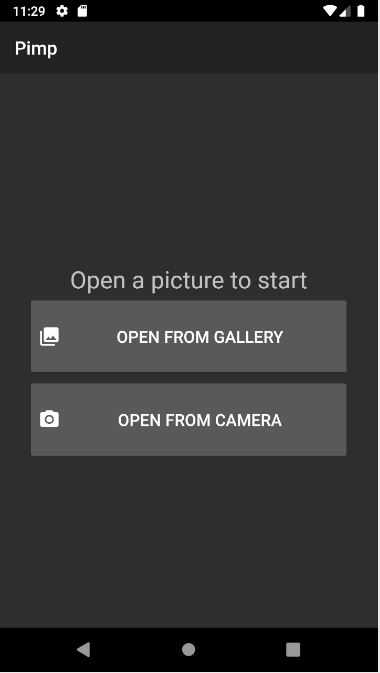
\includegraphics[width=1\textwidth]{report_src/app_manual/first_activity_preview.JPG}
    \end{minipage}
    \begin{minipage}{.48\textwidth}
        Appuyez sur le premier bouton (\faPhoto) pour ouvrir votre galerie photo et choisir une image à importer.
        \\

        Ou appuyez sur le second bouton (\faCamera) pour ouvrir la caméra de votre appareil Android. Capturez alors une image, elle sera sauvegardée dans votre galerie et instantanément importée dans l'application.
        \\

        Il sera nécessaire à la toute première utilisation de ces fonctionnalités d'autoriser l'application à accéder à la galerie et/ou la caméra.
    \end{minipage}
\end{center}
\clearpage

Après avoir choisi une image vous accéderez à la page d'édition principale :
\begin{center}
    \begin{minipage}{.48\textwidth}
      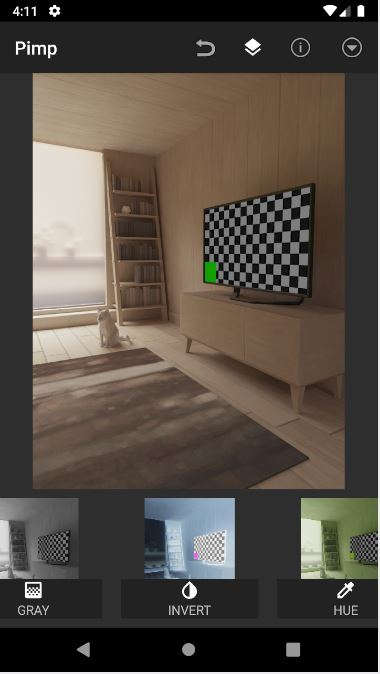
\includegraphics[width=1\textwidth]{report_src/app_manual/main_activity_preview.JPG}
    \end{minipage}
    \begin{minipage}{.48\textwidth}
        Il vous sera possible d'importer une nouvelle image depuis le menu {\faChevronCircleDown}  en haut à droite :
        \begin{center}
        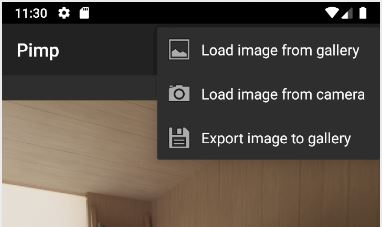
\includegraphics[width=0.8\textwidth]{report_src/app_manual/3dot_button_preview.JPG}
        \end{center}    

        Le bouton {\faSave} permettra d'exporter votre image dans votre galerie, cette opération peut prendre un peu de temps car l'image exportée sera de même taille que l'image d'origine.
        \\

        Vous pouvez manipuler l'image, glissez pour la déplacer et pincez pour zoomer ou dé-zoomer.
    \end{minipage}
\end{center}

En bas de l'écran vous trouverez la liste des effets disponibles applicables sur votre image, faites défiler de droite à gauche.
\\

Le bouton {\faMailReply} annule tout les changements appliqués à l'image en la restaurant à son état d'origine.
\clearpage

Le bouton {\faInfoCircle} quand à lui affiche les informations suivantes à propos de l'image :
\begin{center}
    \begin{minipage}{.48\textwidth}
      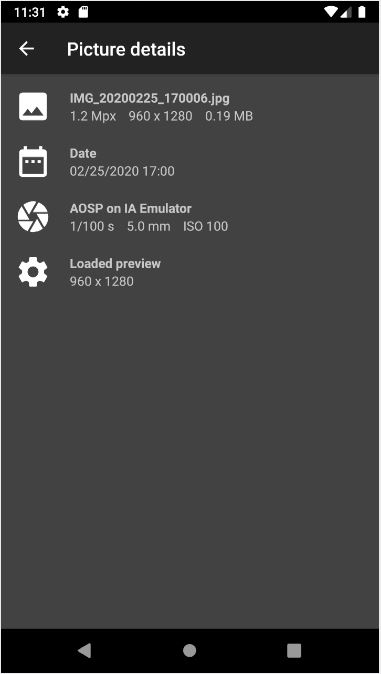
\includegraphics[width=1\textwidth]{report_src/app_manual/info_fragment_preview.JPG}
    \end{minipage}
    \begin{minipage}{.48\textwidth}
        Les sections {\faPhoto} {\faCalendar} {\faChrome} et {\faMapMarker} permettent d'afficher des informations respectivement sur le fichier image, sur sa date de prise de vue, sur l'appareil source et sur ses coordonnées géographiques.
        \\
        Ces sections ne sont pas toujours visibles et dépendent du fichier image.
        \\

        Quand à la section {\faCog} elle donne les dimensions de l'aperçu actuellement affiché dans l'application, il peut être plus petit que l'image d'origine afin de préserver la mémoire du téléphone et le temps d'exécution. L'image exportée en revanche sera aux bonnes dimensions.
    \end{minipage}
\end{center}
\clearpage

Après avoir sélectionné un effet sur la liste en bas de l'écran, des éléments d'interface vont se superposer à votre image :
\begin{center}
    \begin{minipage}{.48\textwidth}
      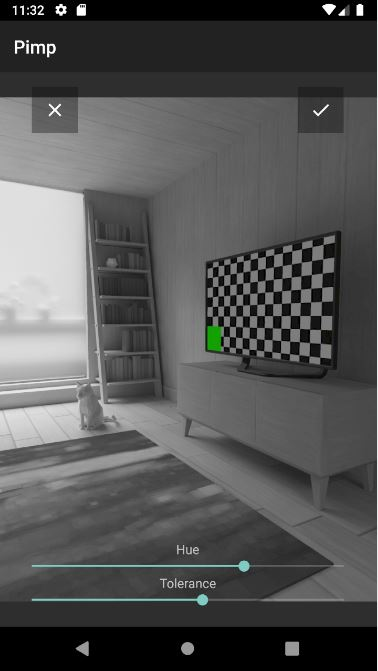
\includegraphics[width=1\textwidth]{report_src/app_manual/effect_fragment_preview.JPG}
    \end{minipage}
    \begin{minipage}{.48\textwidth}
        Le bouton {\faRemove} en haut à gauche vous fait revenir à la liste d'effets et annule l'effet courant.
        \\

        Le bouton {\faCheck} en haut à droite applique l'effet et vous fait revenir à la liste d'effets.
        \\

        En bas des curseurs ou des boutons peuvent apparaître, selon l'effet sélectionné. Manipulez les pour voir en temps réel l'impact sur l'image.
    \end{minipage}
\end{center}

\vspace{2cm}
\textbf{NB:} L'entièreté de cette application est verrouillée en mode portrait.

\clearpage

%%%%%%%%%%%%%%%%%%%%%%%%%%%%%%%%%%%%%%%%%%%%%%%%%%%%%
% Effets disponibles :
%%%%%%%%%%%%%%%%%%%%%%%%%%%%%%%%%%%%%%%%%%%%%%%%%%%%%
\section{Effets :}
\textbf{NB:} Tous les effets nécessitant un histogramme utilise celui de la "\emph{valeur}", soit le maximum entre les trois canaux de l'espace de couleur Rouge Vert Bleu.

\subsection{Luminosité (Brightness) :}
\begin{figure}[!h]
    \centering
    \begin{subfigure}[b]{0.3\textwidth}
        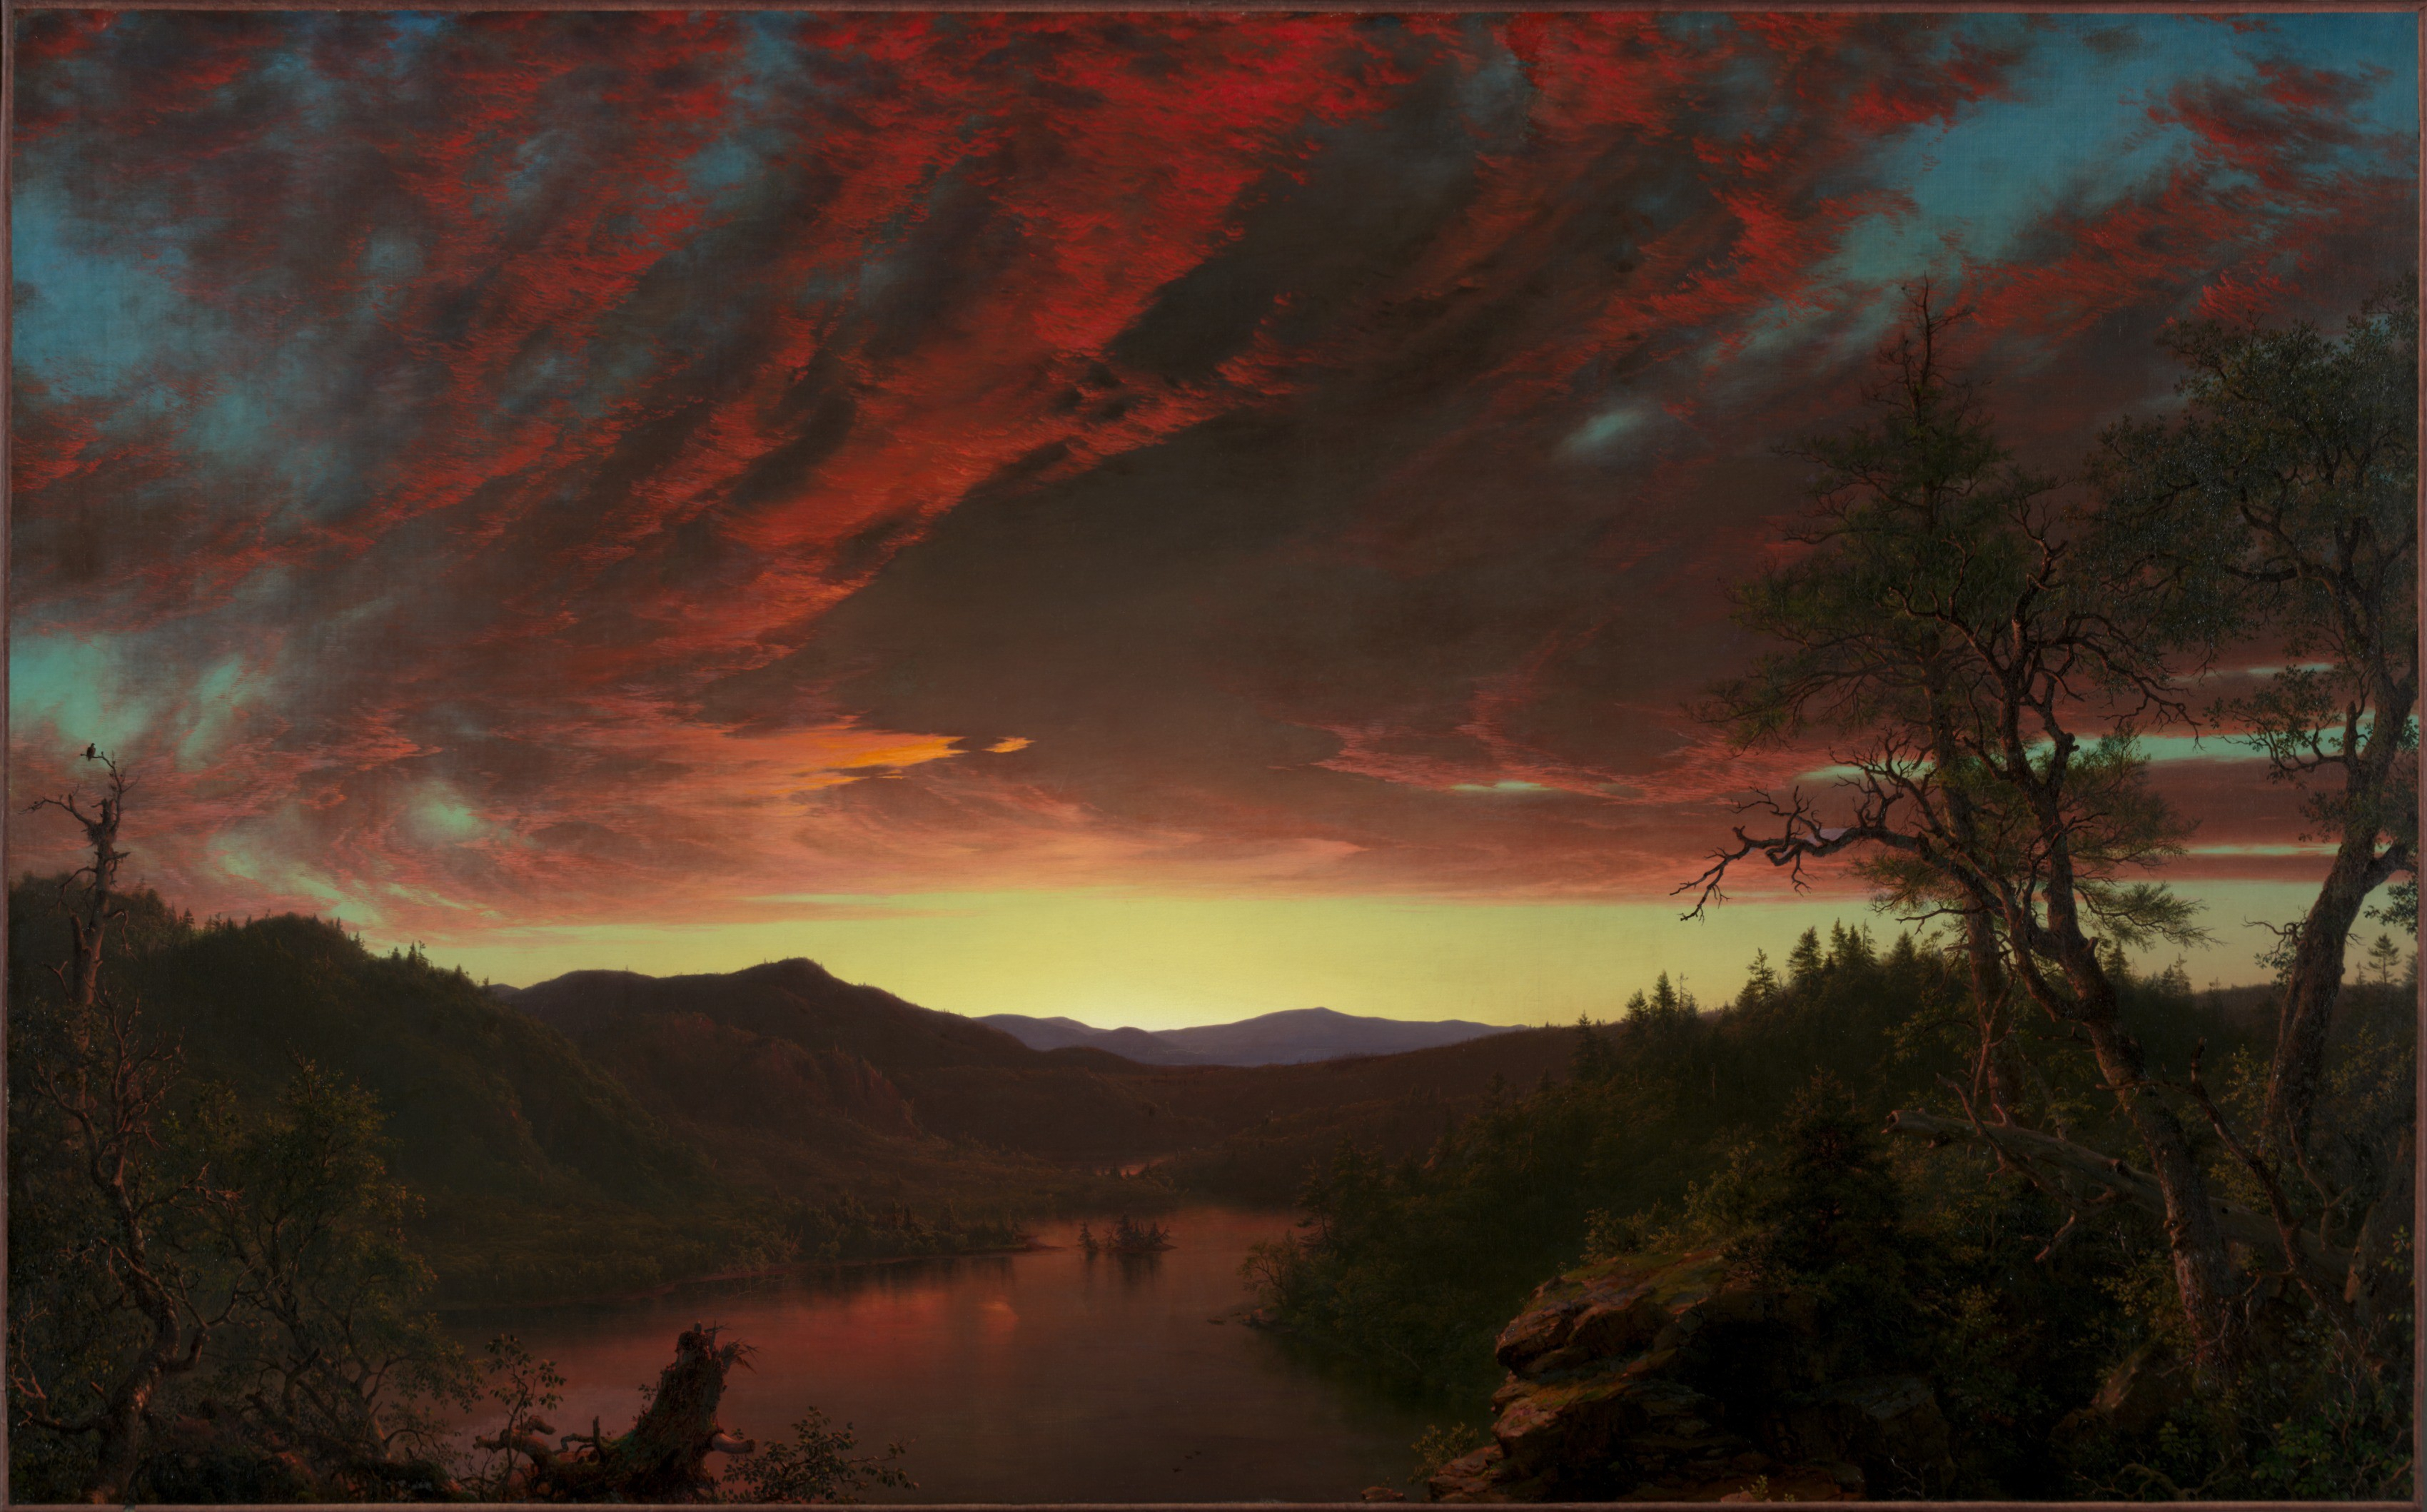
\includegraphics[width=1\textwidth]{report_src/effects/original1.jpeg}
    \end{subfigure}
    \begin{subfigure}[b]{0.3\textwidth}
        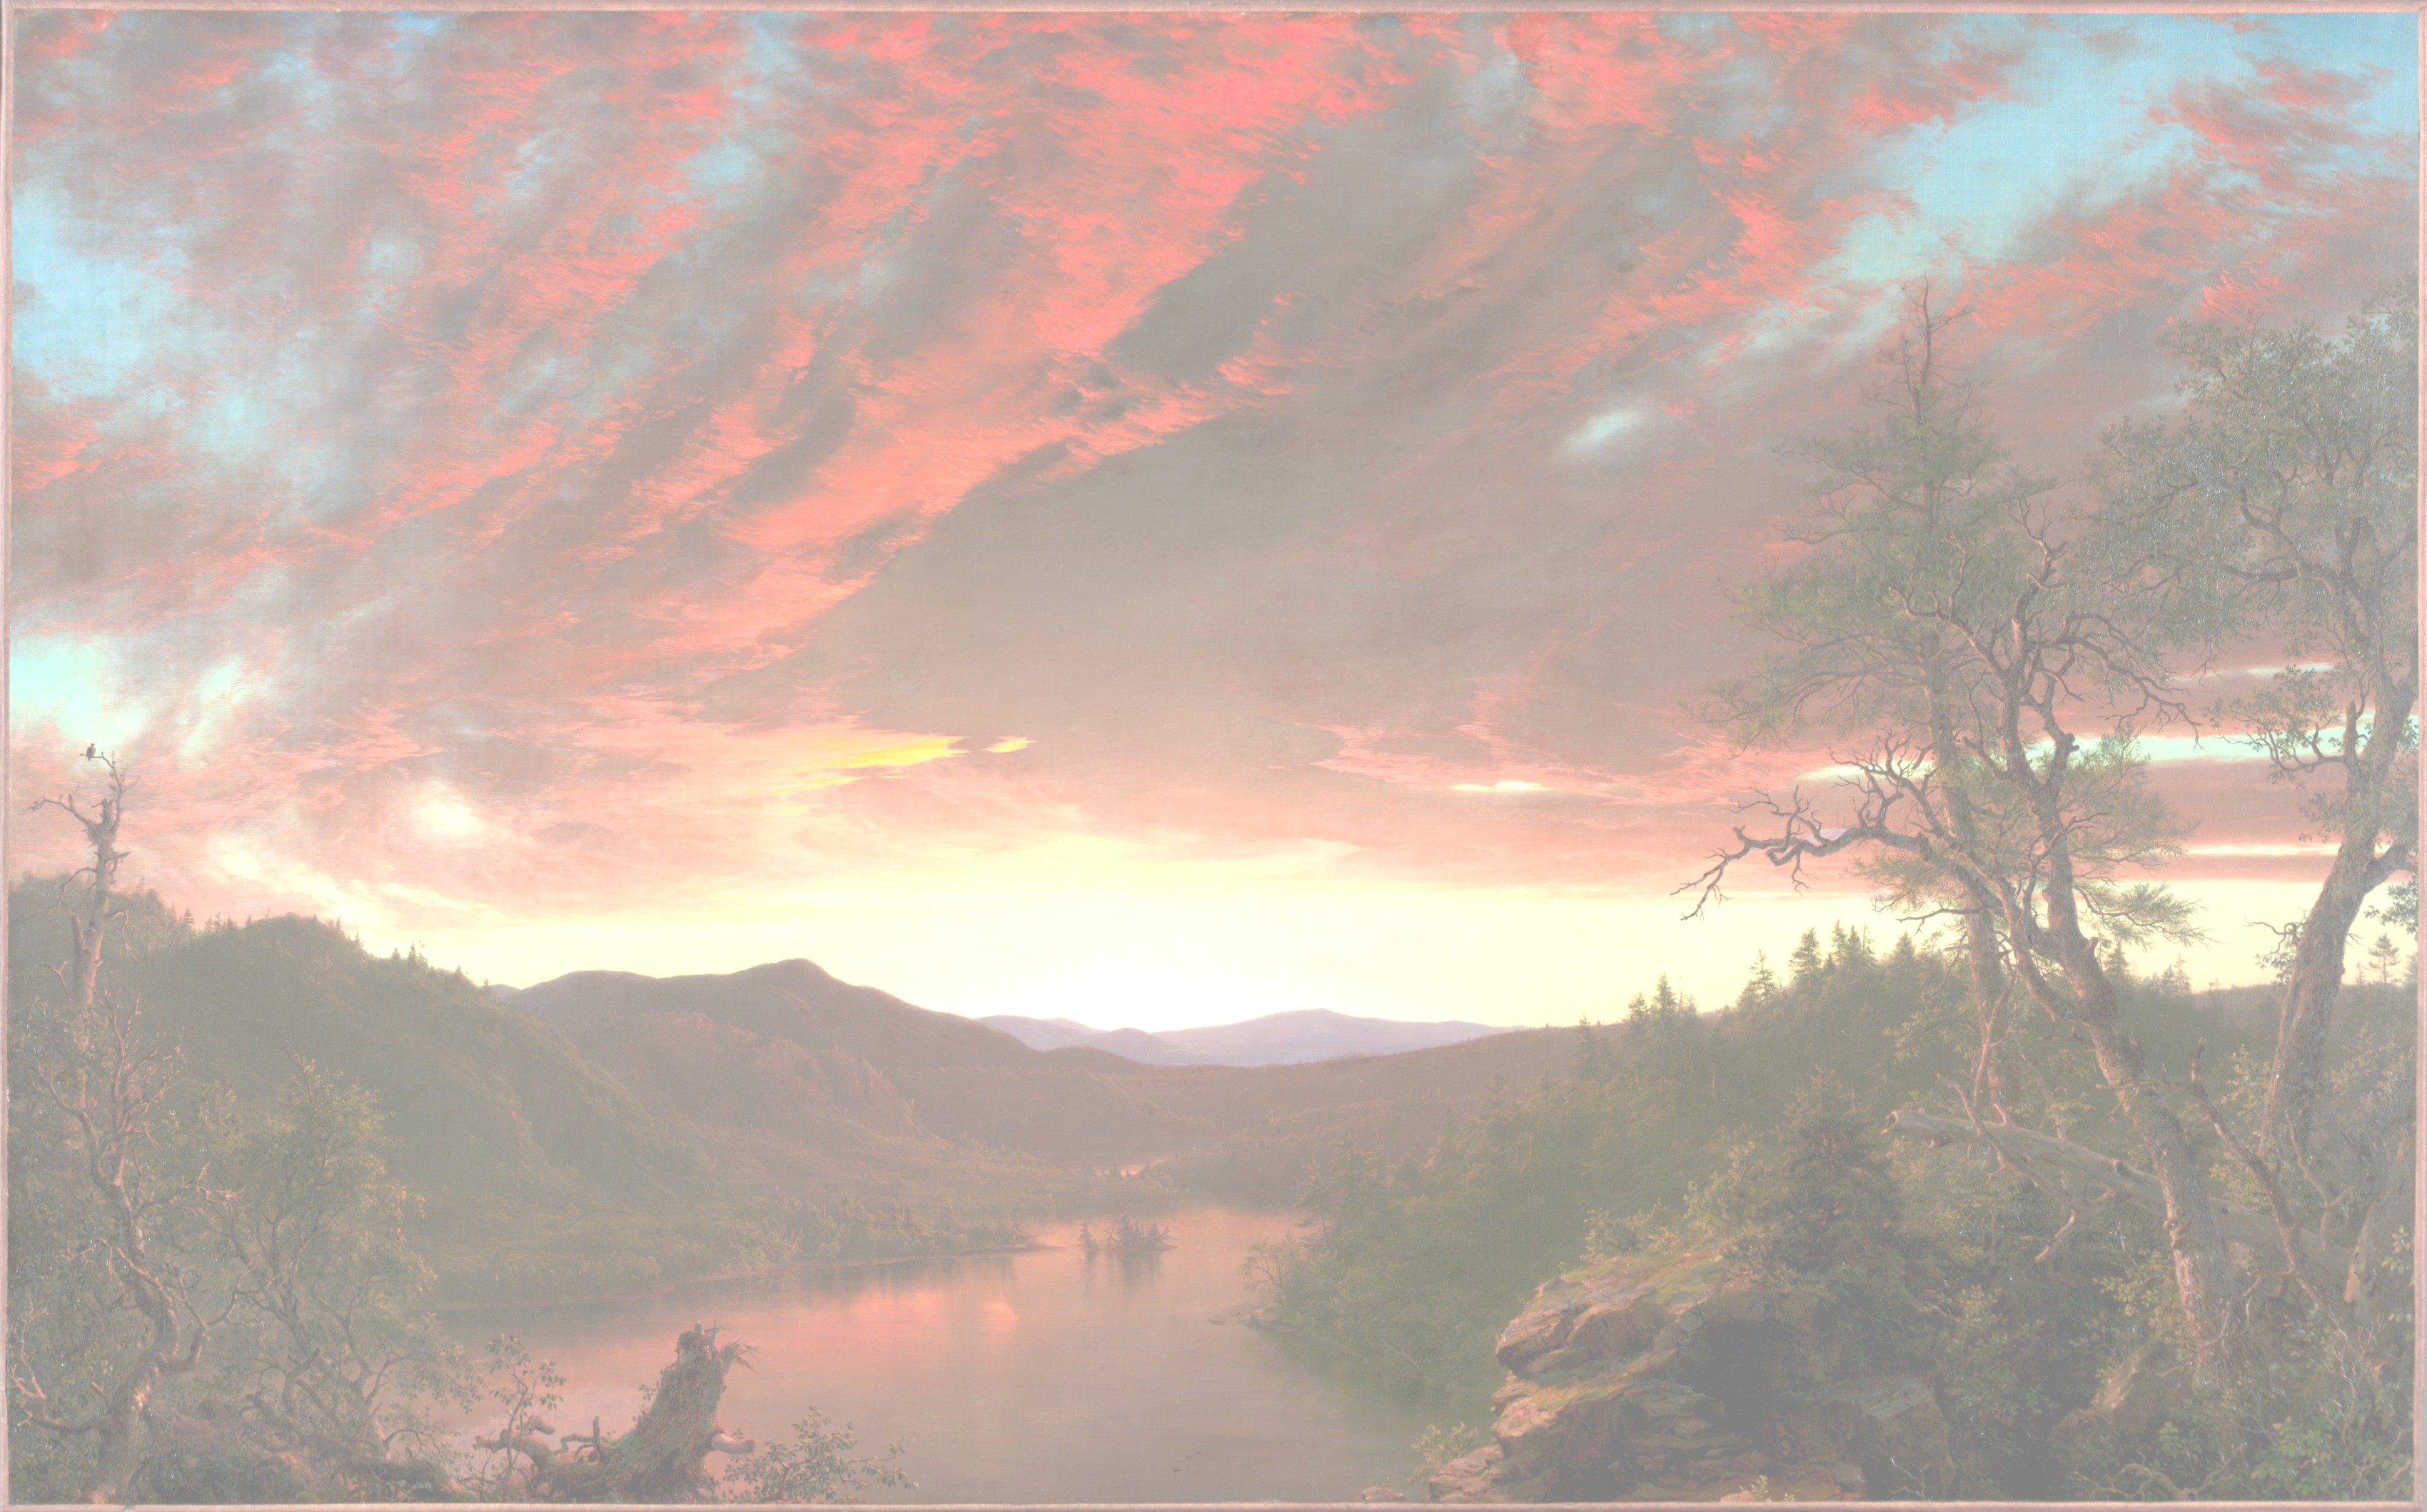
\includegraphics[width=1\textwidth]{report_src/effects/brightness_high.jpeg}
    \end{subfigure}
    \begin{subfigure}[b]{0.3\textwidth}
        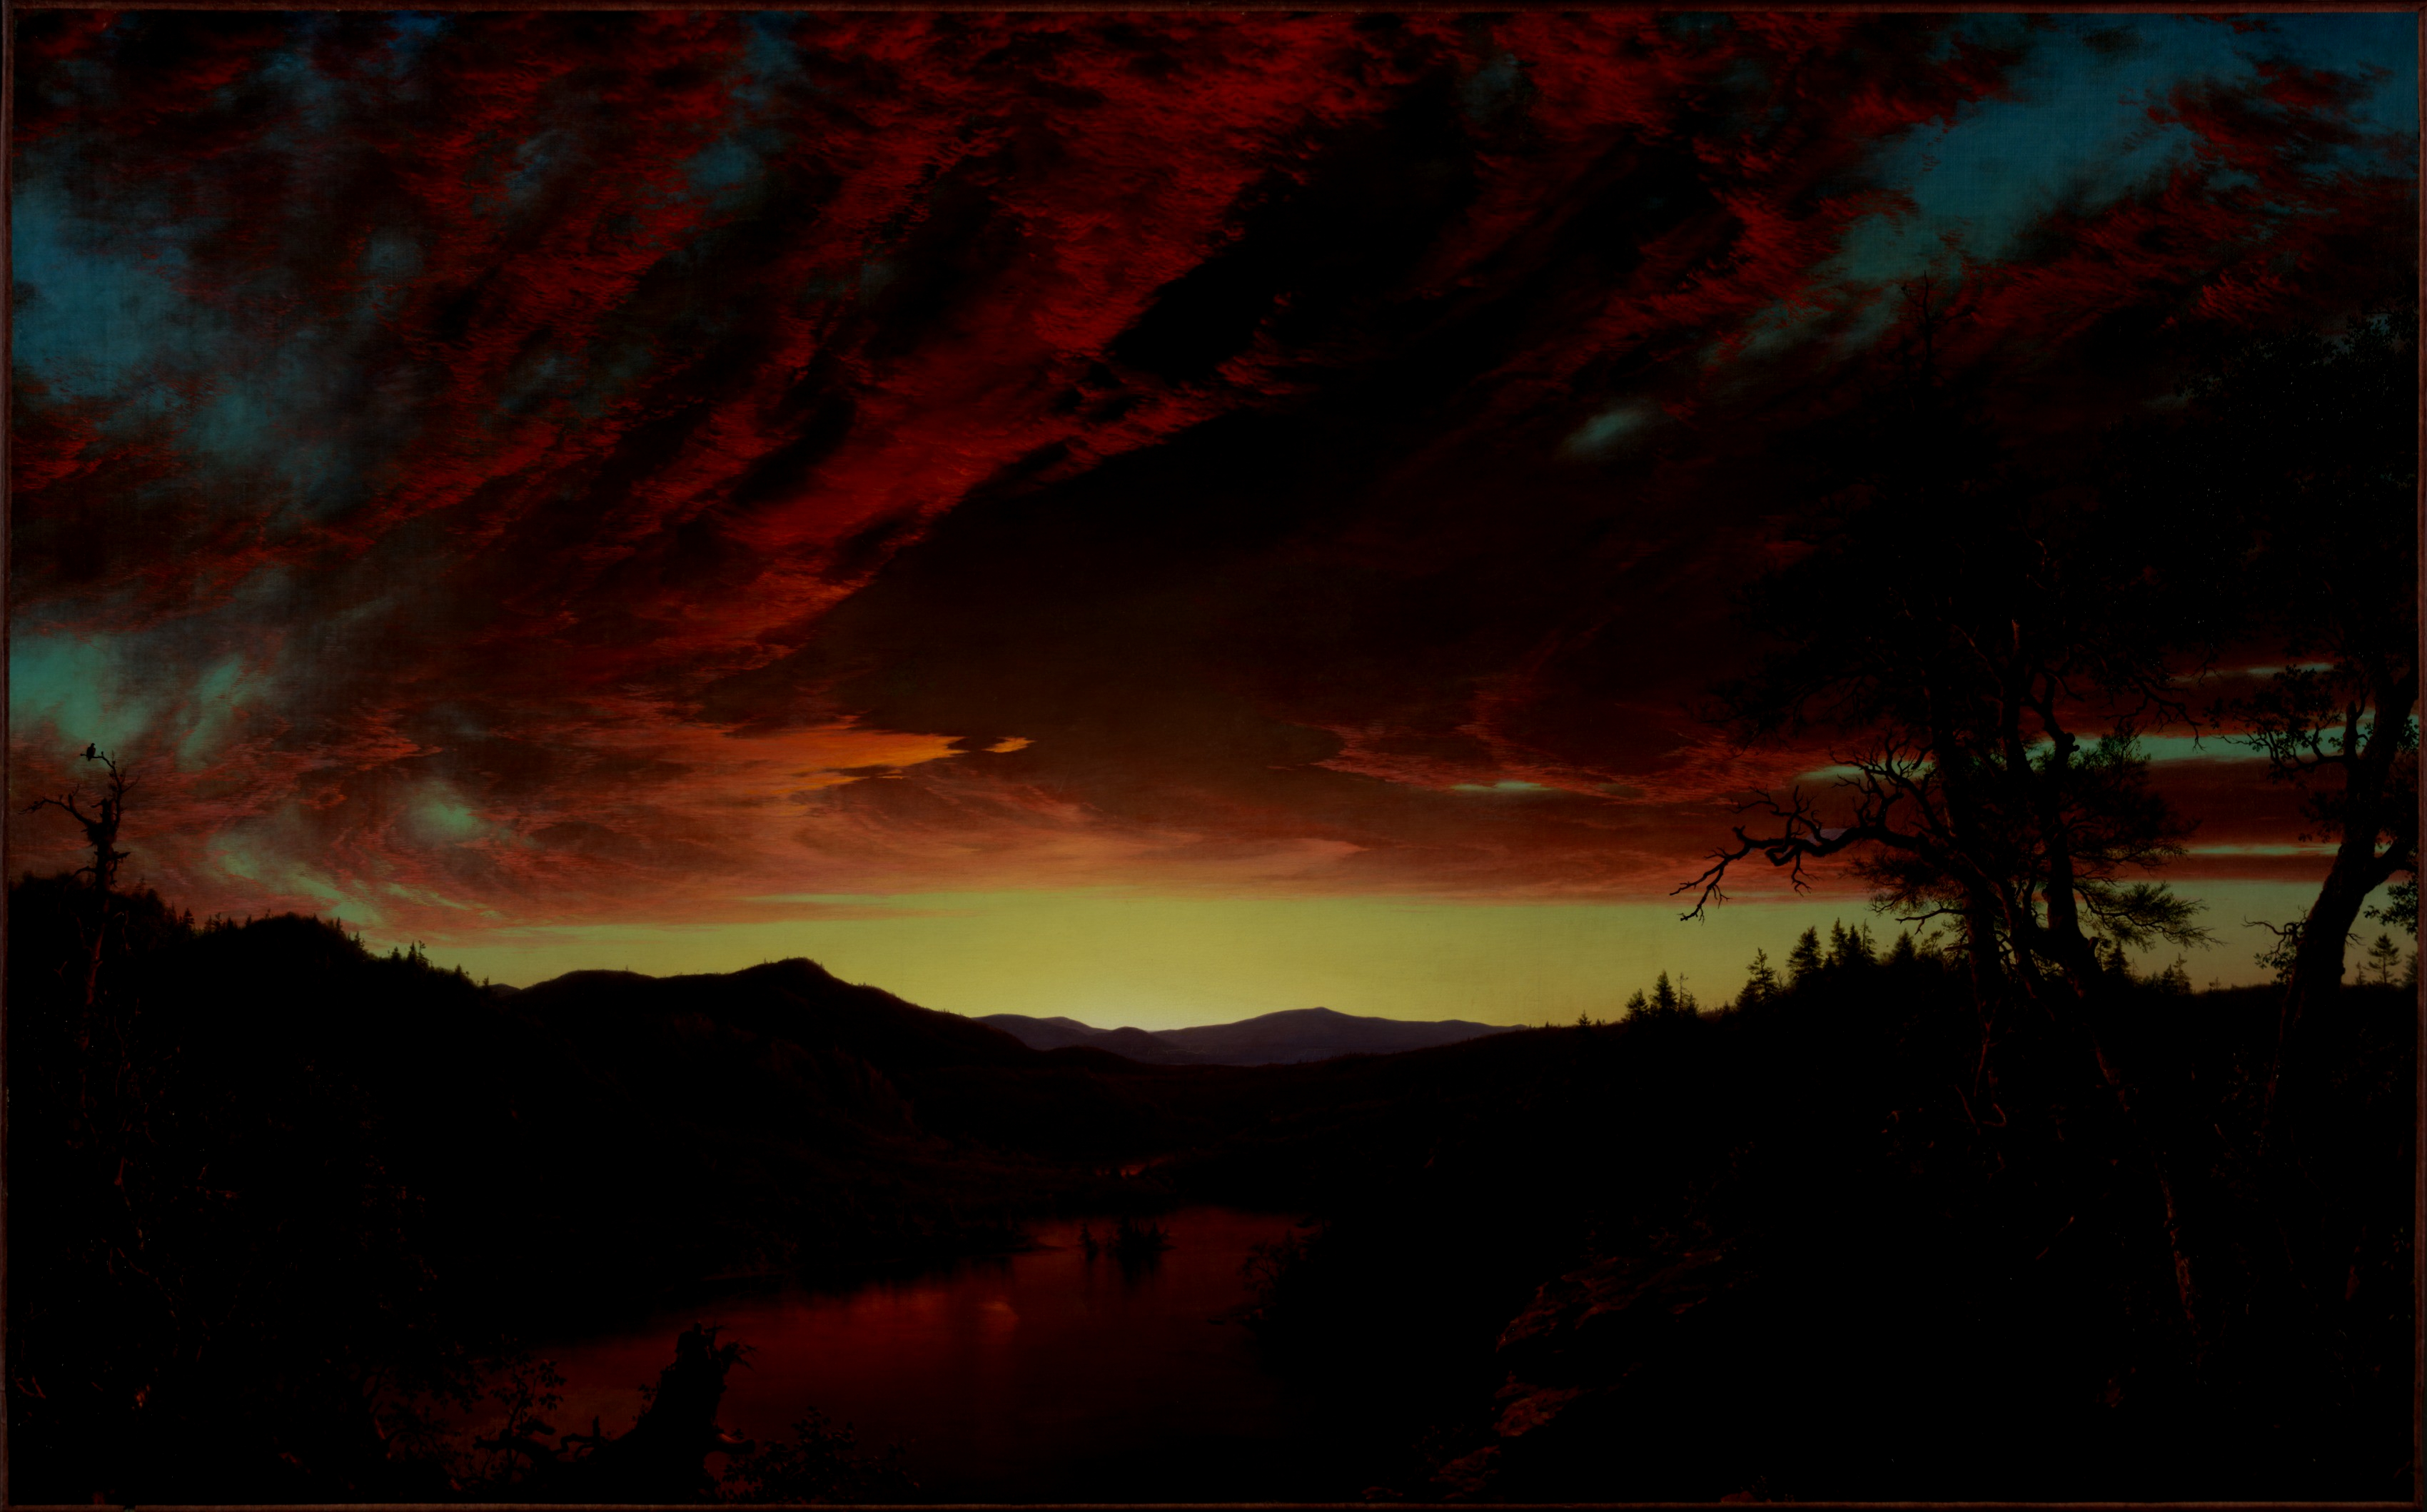
\includegraphics[width=1\textwidth]{report_src/effects/brightness_low.jpeg}
    \end{subfigure}
\end{figure} 

\emph{Méthode appelante : Retouching.setBrightness()}

\emph{Script : brightness.rs}
\\

Ce réglage ajoute une valeur (positive ou négative) aux trois canaux RGB de l'image. Cette valeur est fixée par la seekbar.
Les valeurs sont tronquées entre 0 et 255, par conséquent on perd de l'information dans les valeurs extrêmes de luminosité.

Cet effet n'utilise pas la luminosité existante de l'image, ainsi on peut obtenir des résultats qui sont parfois discutables, par exemple
le noir qui s'éclaircit et inversement pour le blanc. Pour pallier à ce problème, on pourrait introduire une multiplication afin de modifier
la luminosité proportionnellement à celle existante. Cependant, cette solution modifie aussi le contraste, nous avons donc choisi
de laisser l'algorithme tel quel. 


\subsection{Contraste (Contrast) :}

\begin{figure}[!h]
    \centering
    \begin{subfigure}[b]{0.3\textwidth}
        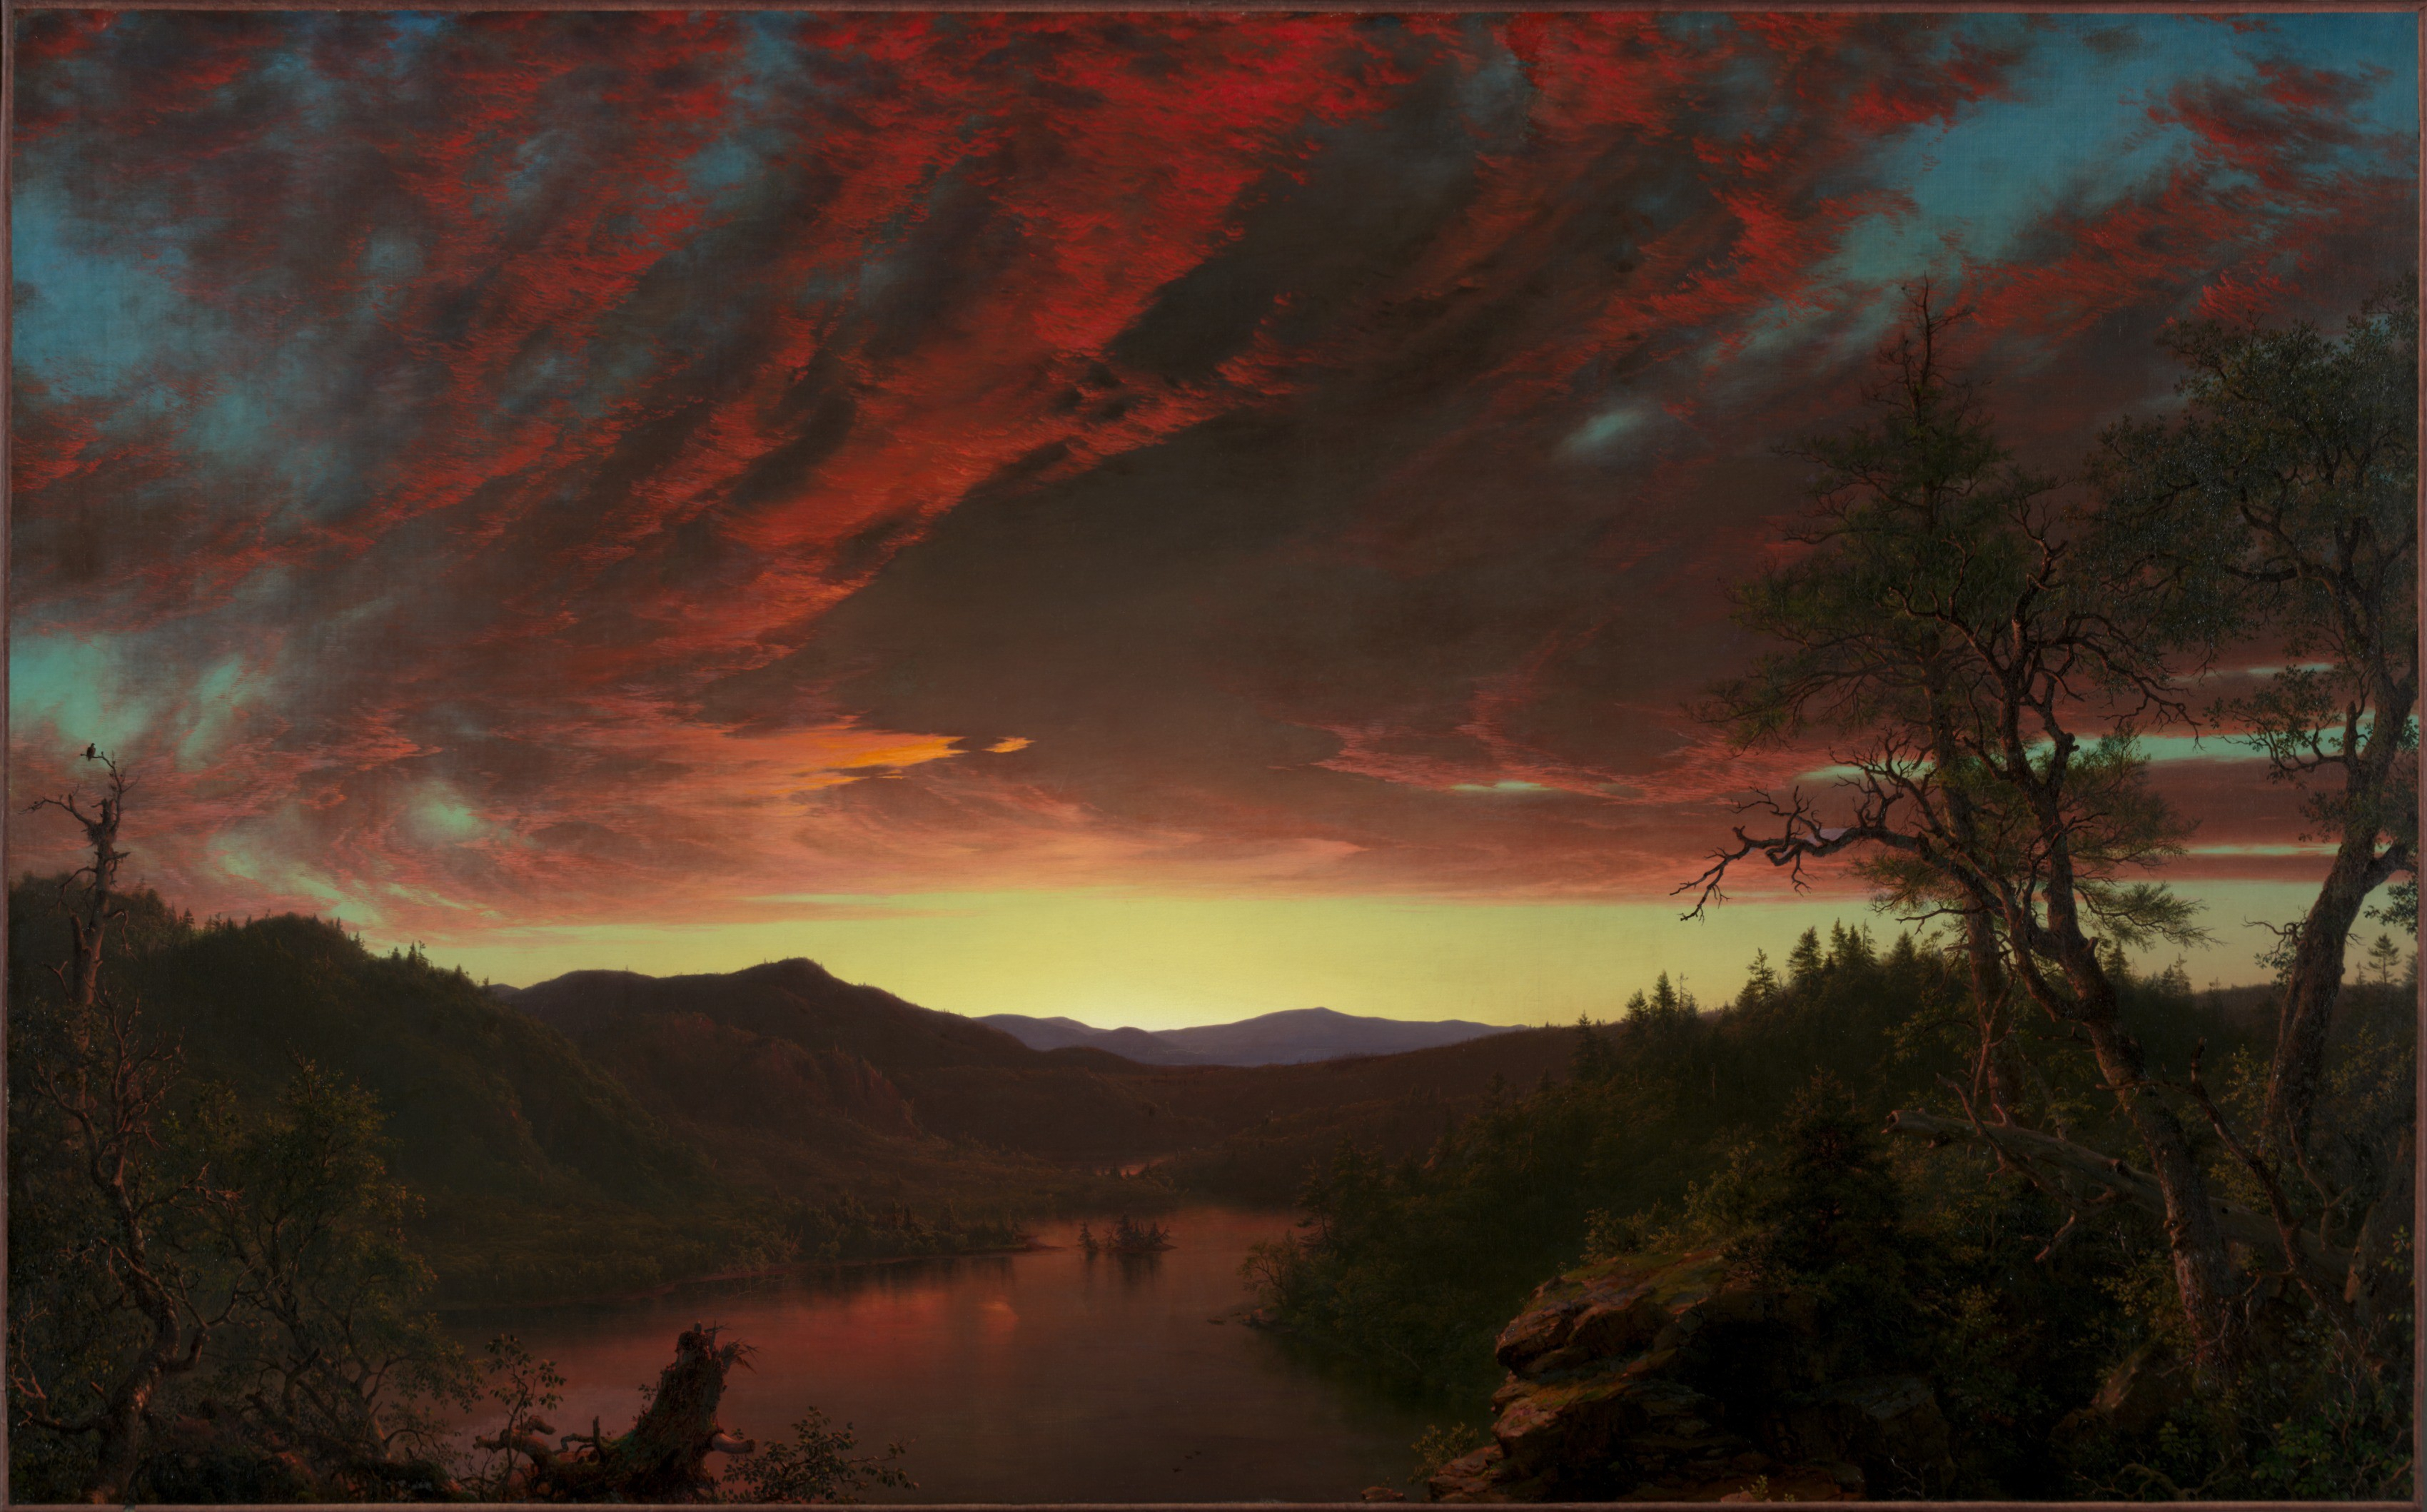
\includegraphics[width=1\textwidth]{report_src/effects/original1.jpeg}
    \end{subfigure}
    \begin{subfigure}[b]{0.3\textwidth}
        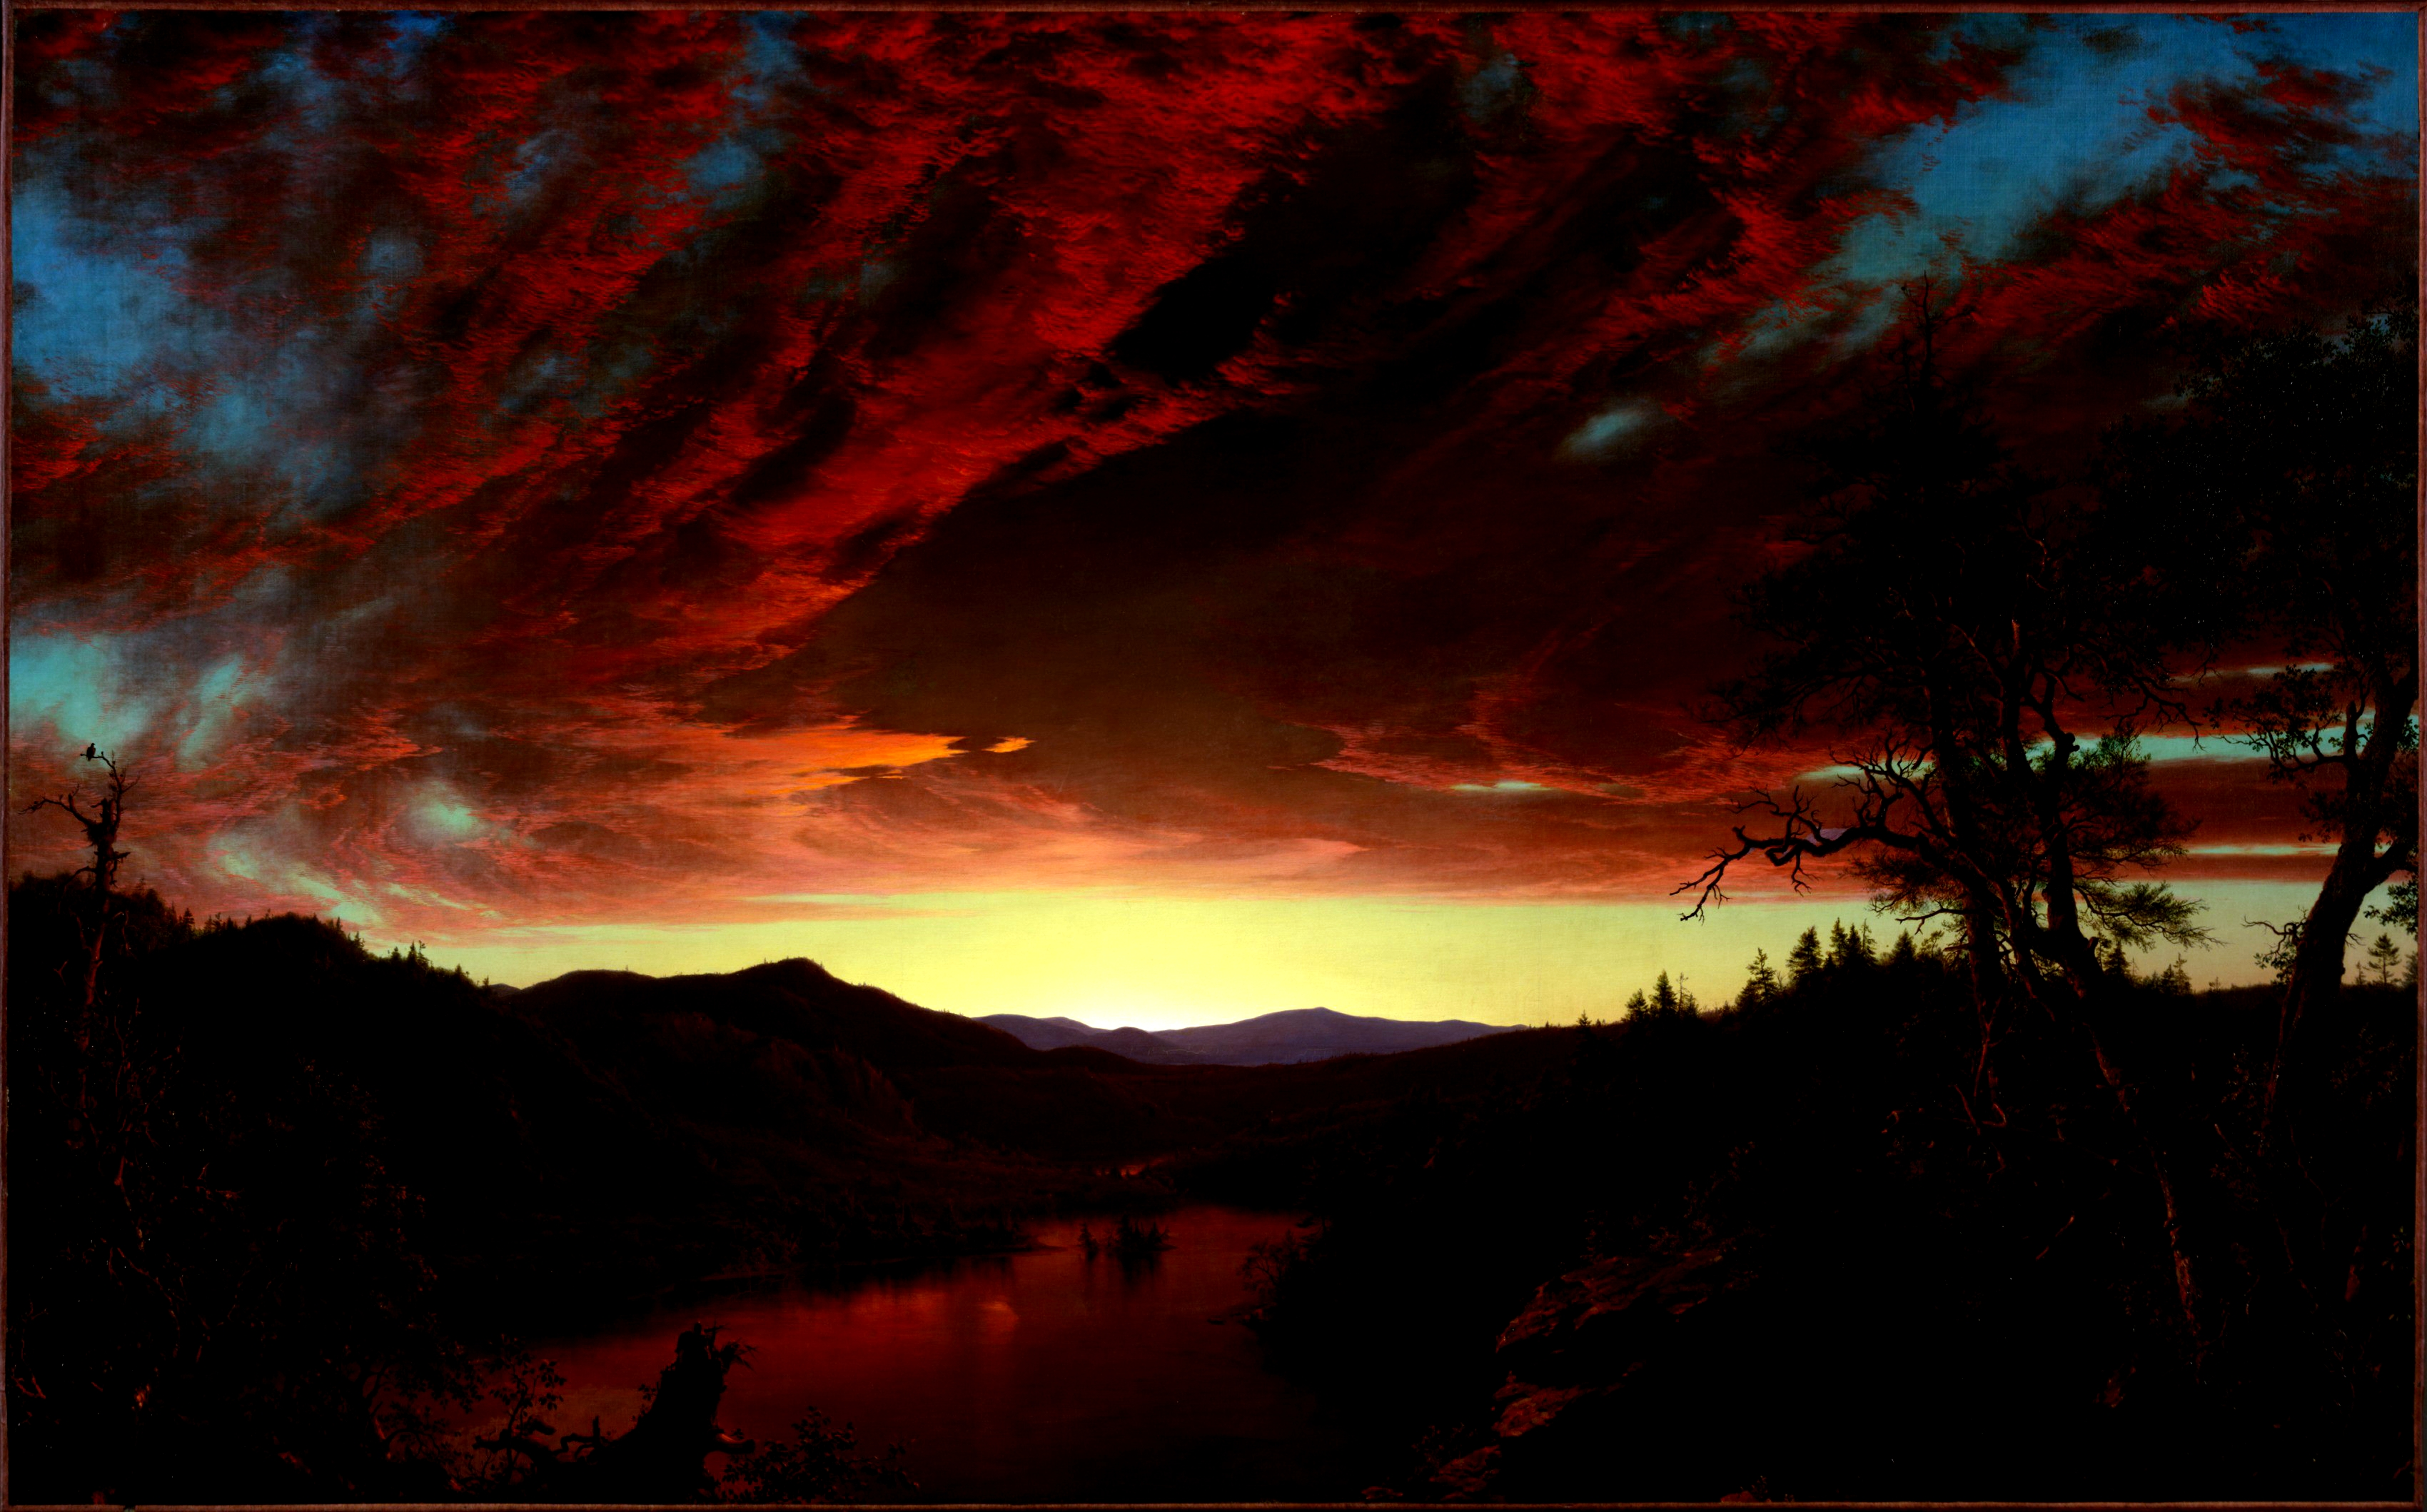
\includegraphics[width=1\textwidth]{report_src/effects/contrast_high.jpeg}
    \end{subfigure}
    \begin{subfigure}[b]{0.3\textwidth}
        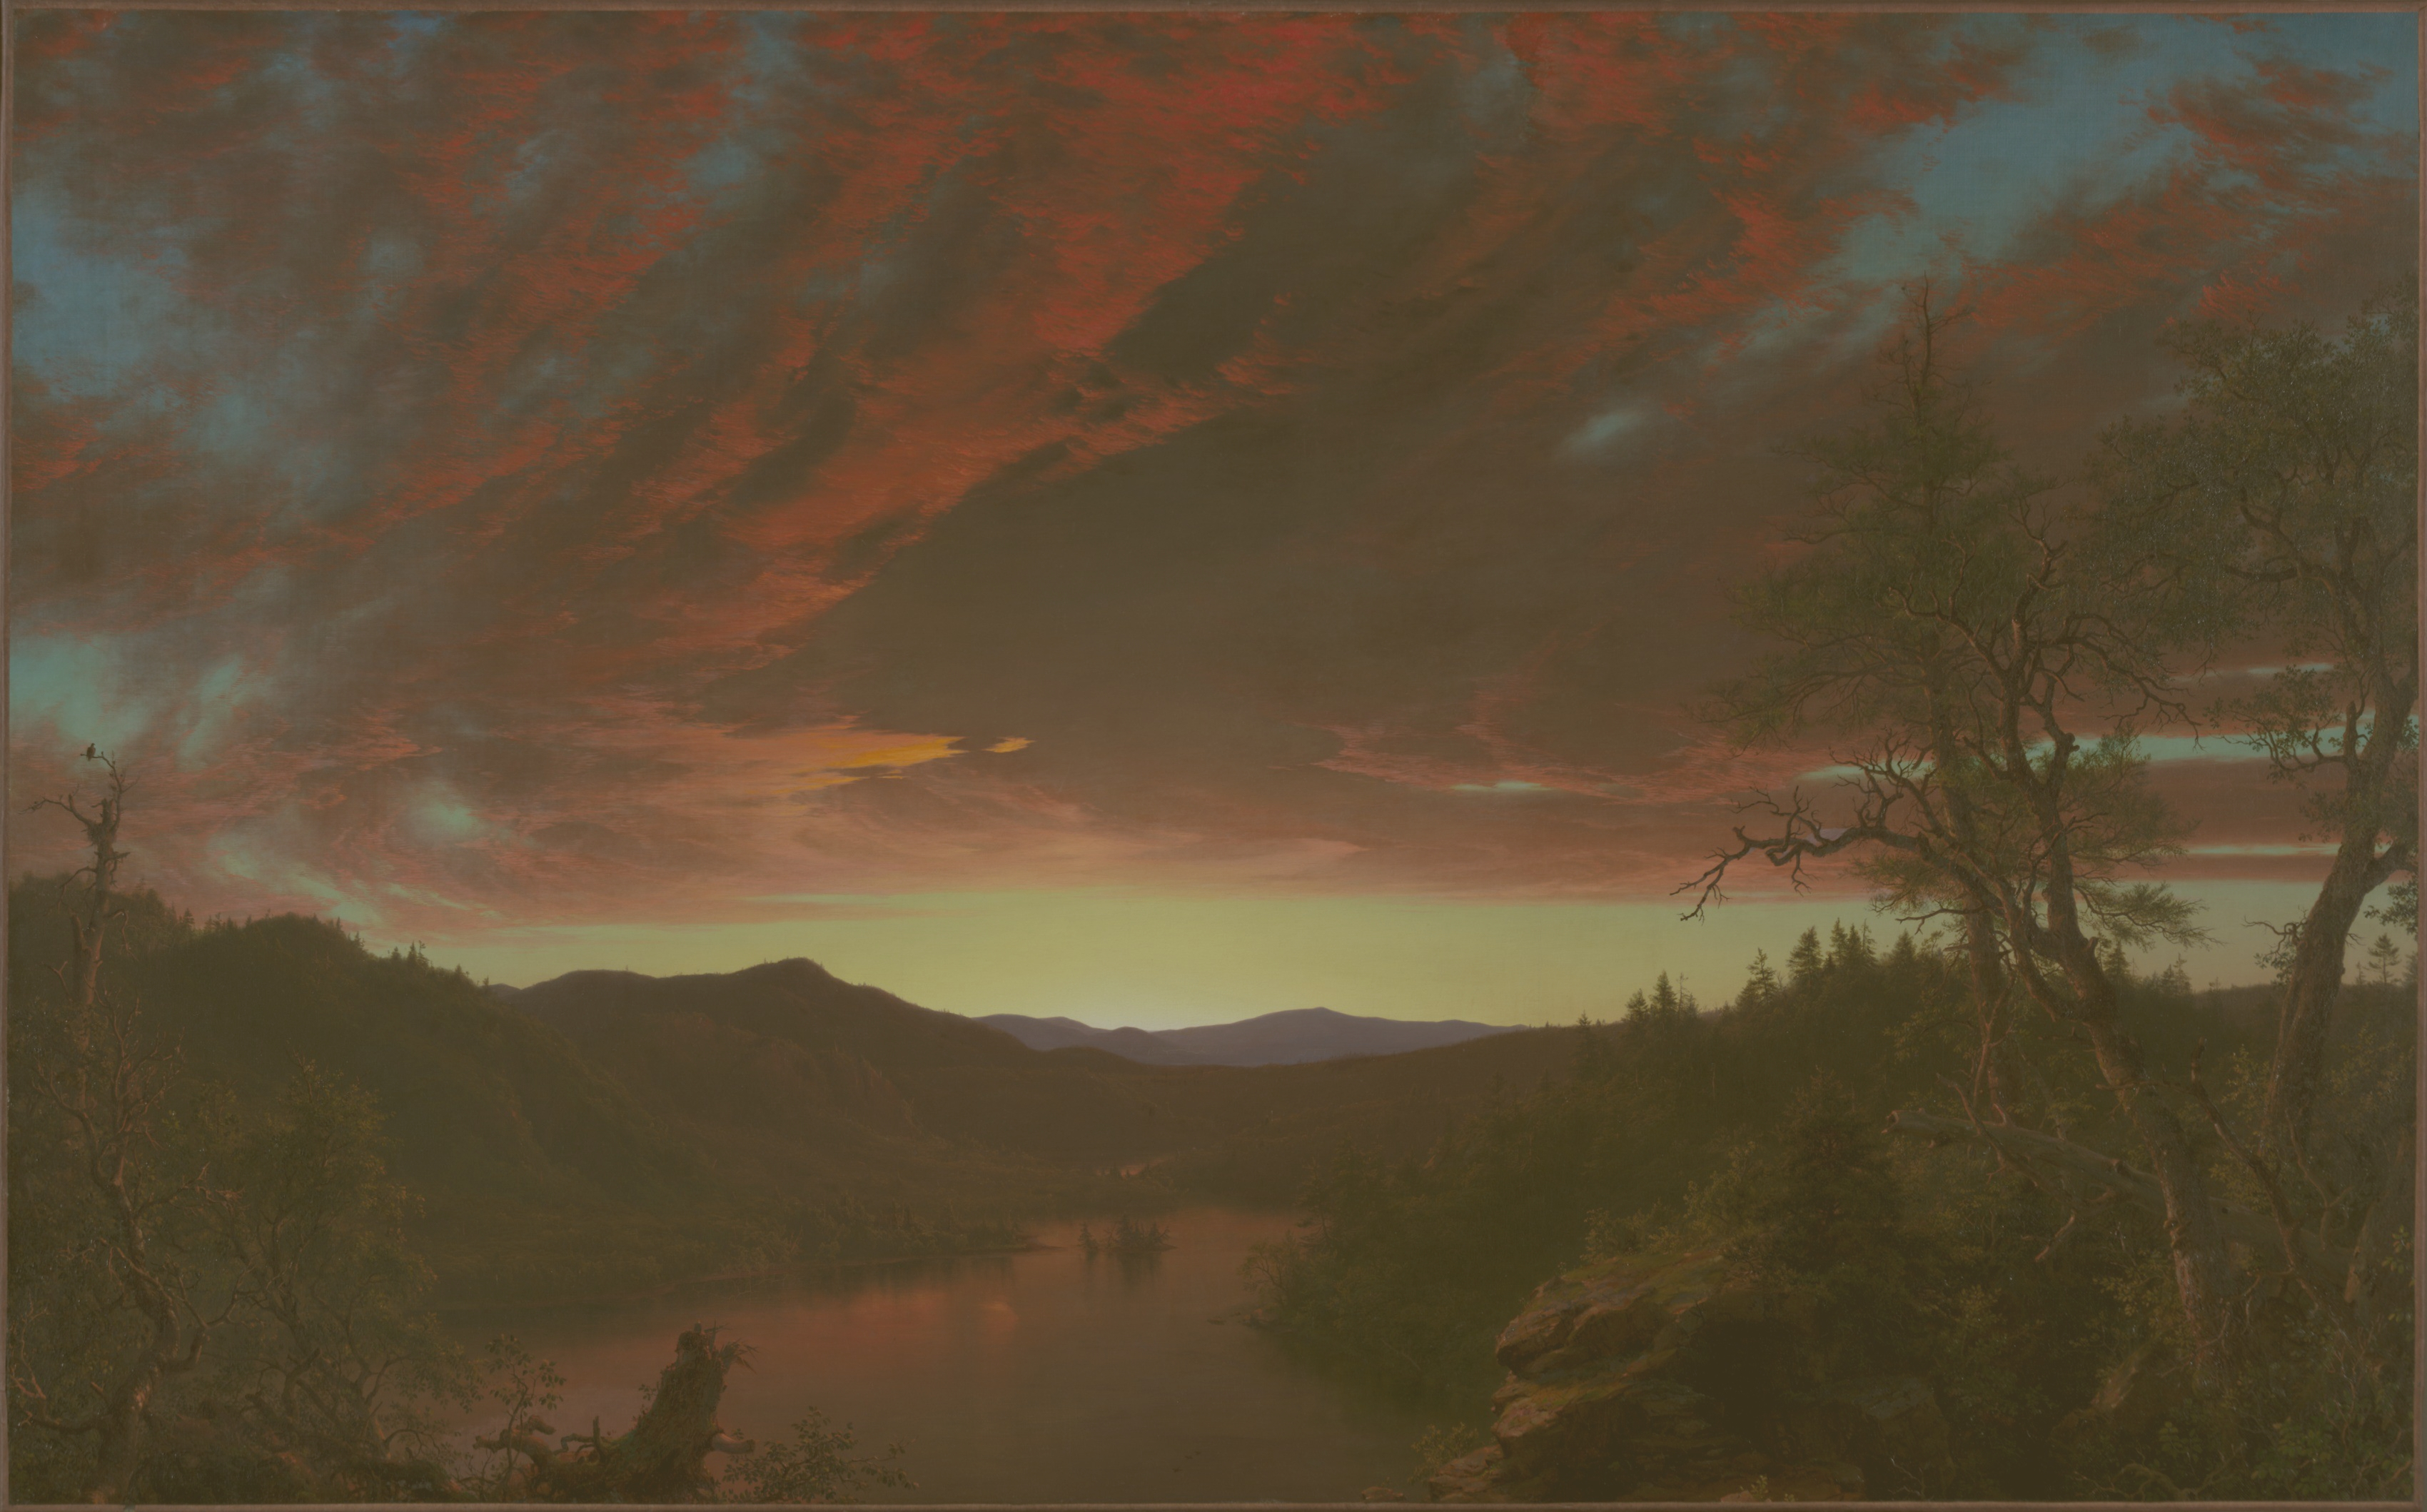
\includegraphics[width=1\textwidth]{report_src/effects/contrast_low.jpeg}
    \end{subfigure}
\end{figure} 

\emph{Méthode appelante : Retouching.dynamicExtensionRGB()}

\emph{Script : dynamicExtension.rs}
\\ 

Ce réglage effectue une extension linéaire de dynamique. Les nouveaux extremum de l'histogramme sont définis à partir de la position de la seekbar.
La dynamique est ainsi étendue autour d'une valeur se situant au milieu des deux anciens extremum de l'histogramme*. On a donc une image uniforme lorsque
l'on règle le contraste au minimum. En augmentant le contraste, les extremum peuvent sortir de l'intervalle [0;255], ce qui provoque une distorsion de l'image.
\\

*Il serait peut-être plus judicieux de prendre la médiane de l'histogramme cumulé afin d'avoir une valeur qui représente mieux la "valeur moyenne" de l'image.


\subsection{Saturation (Saturation) :}

\begin{figure}[!h]
    \centering
    \begin{subfigure}[b]{0.3\textwidth}
        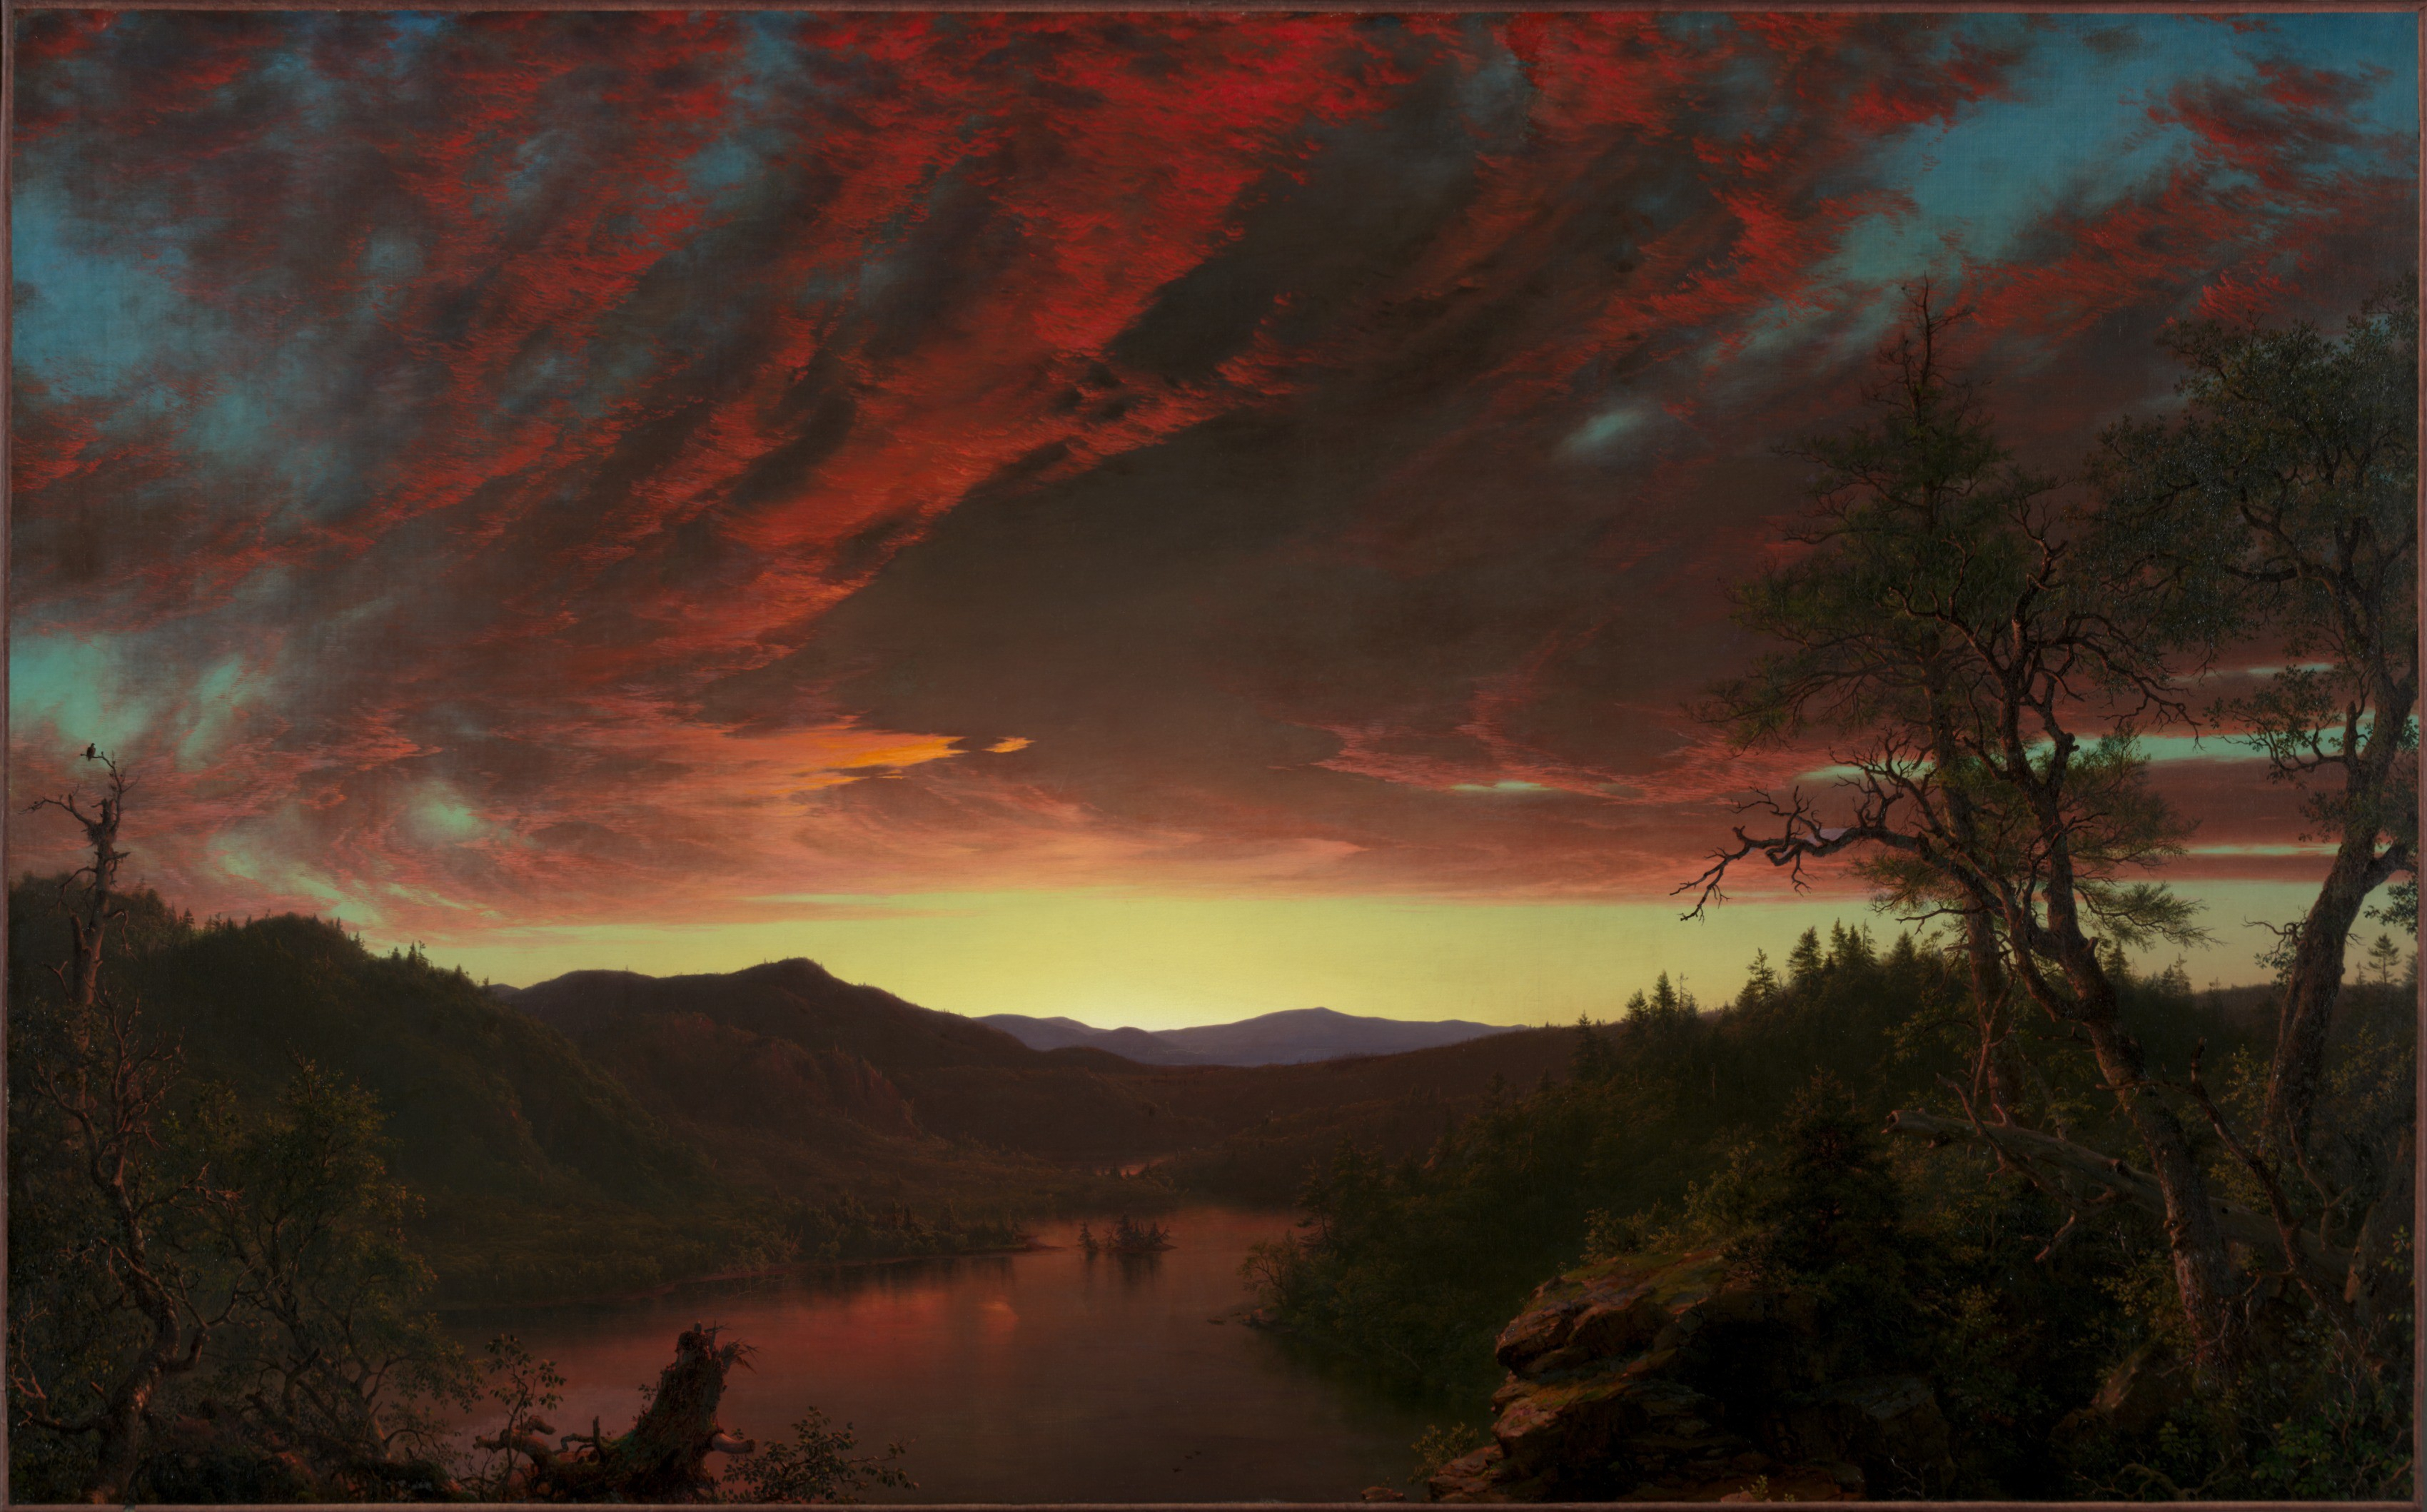
\includegraphics[width=1\textwidth]{report_src/effects/original1.jpeg}
    \end{subfigure}
    \begin{subfigure}[b]{0.3\textwidth}
        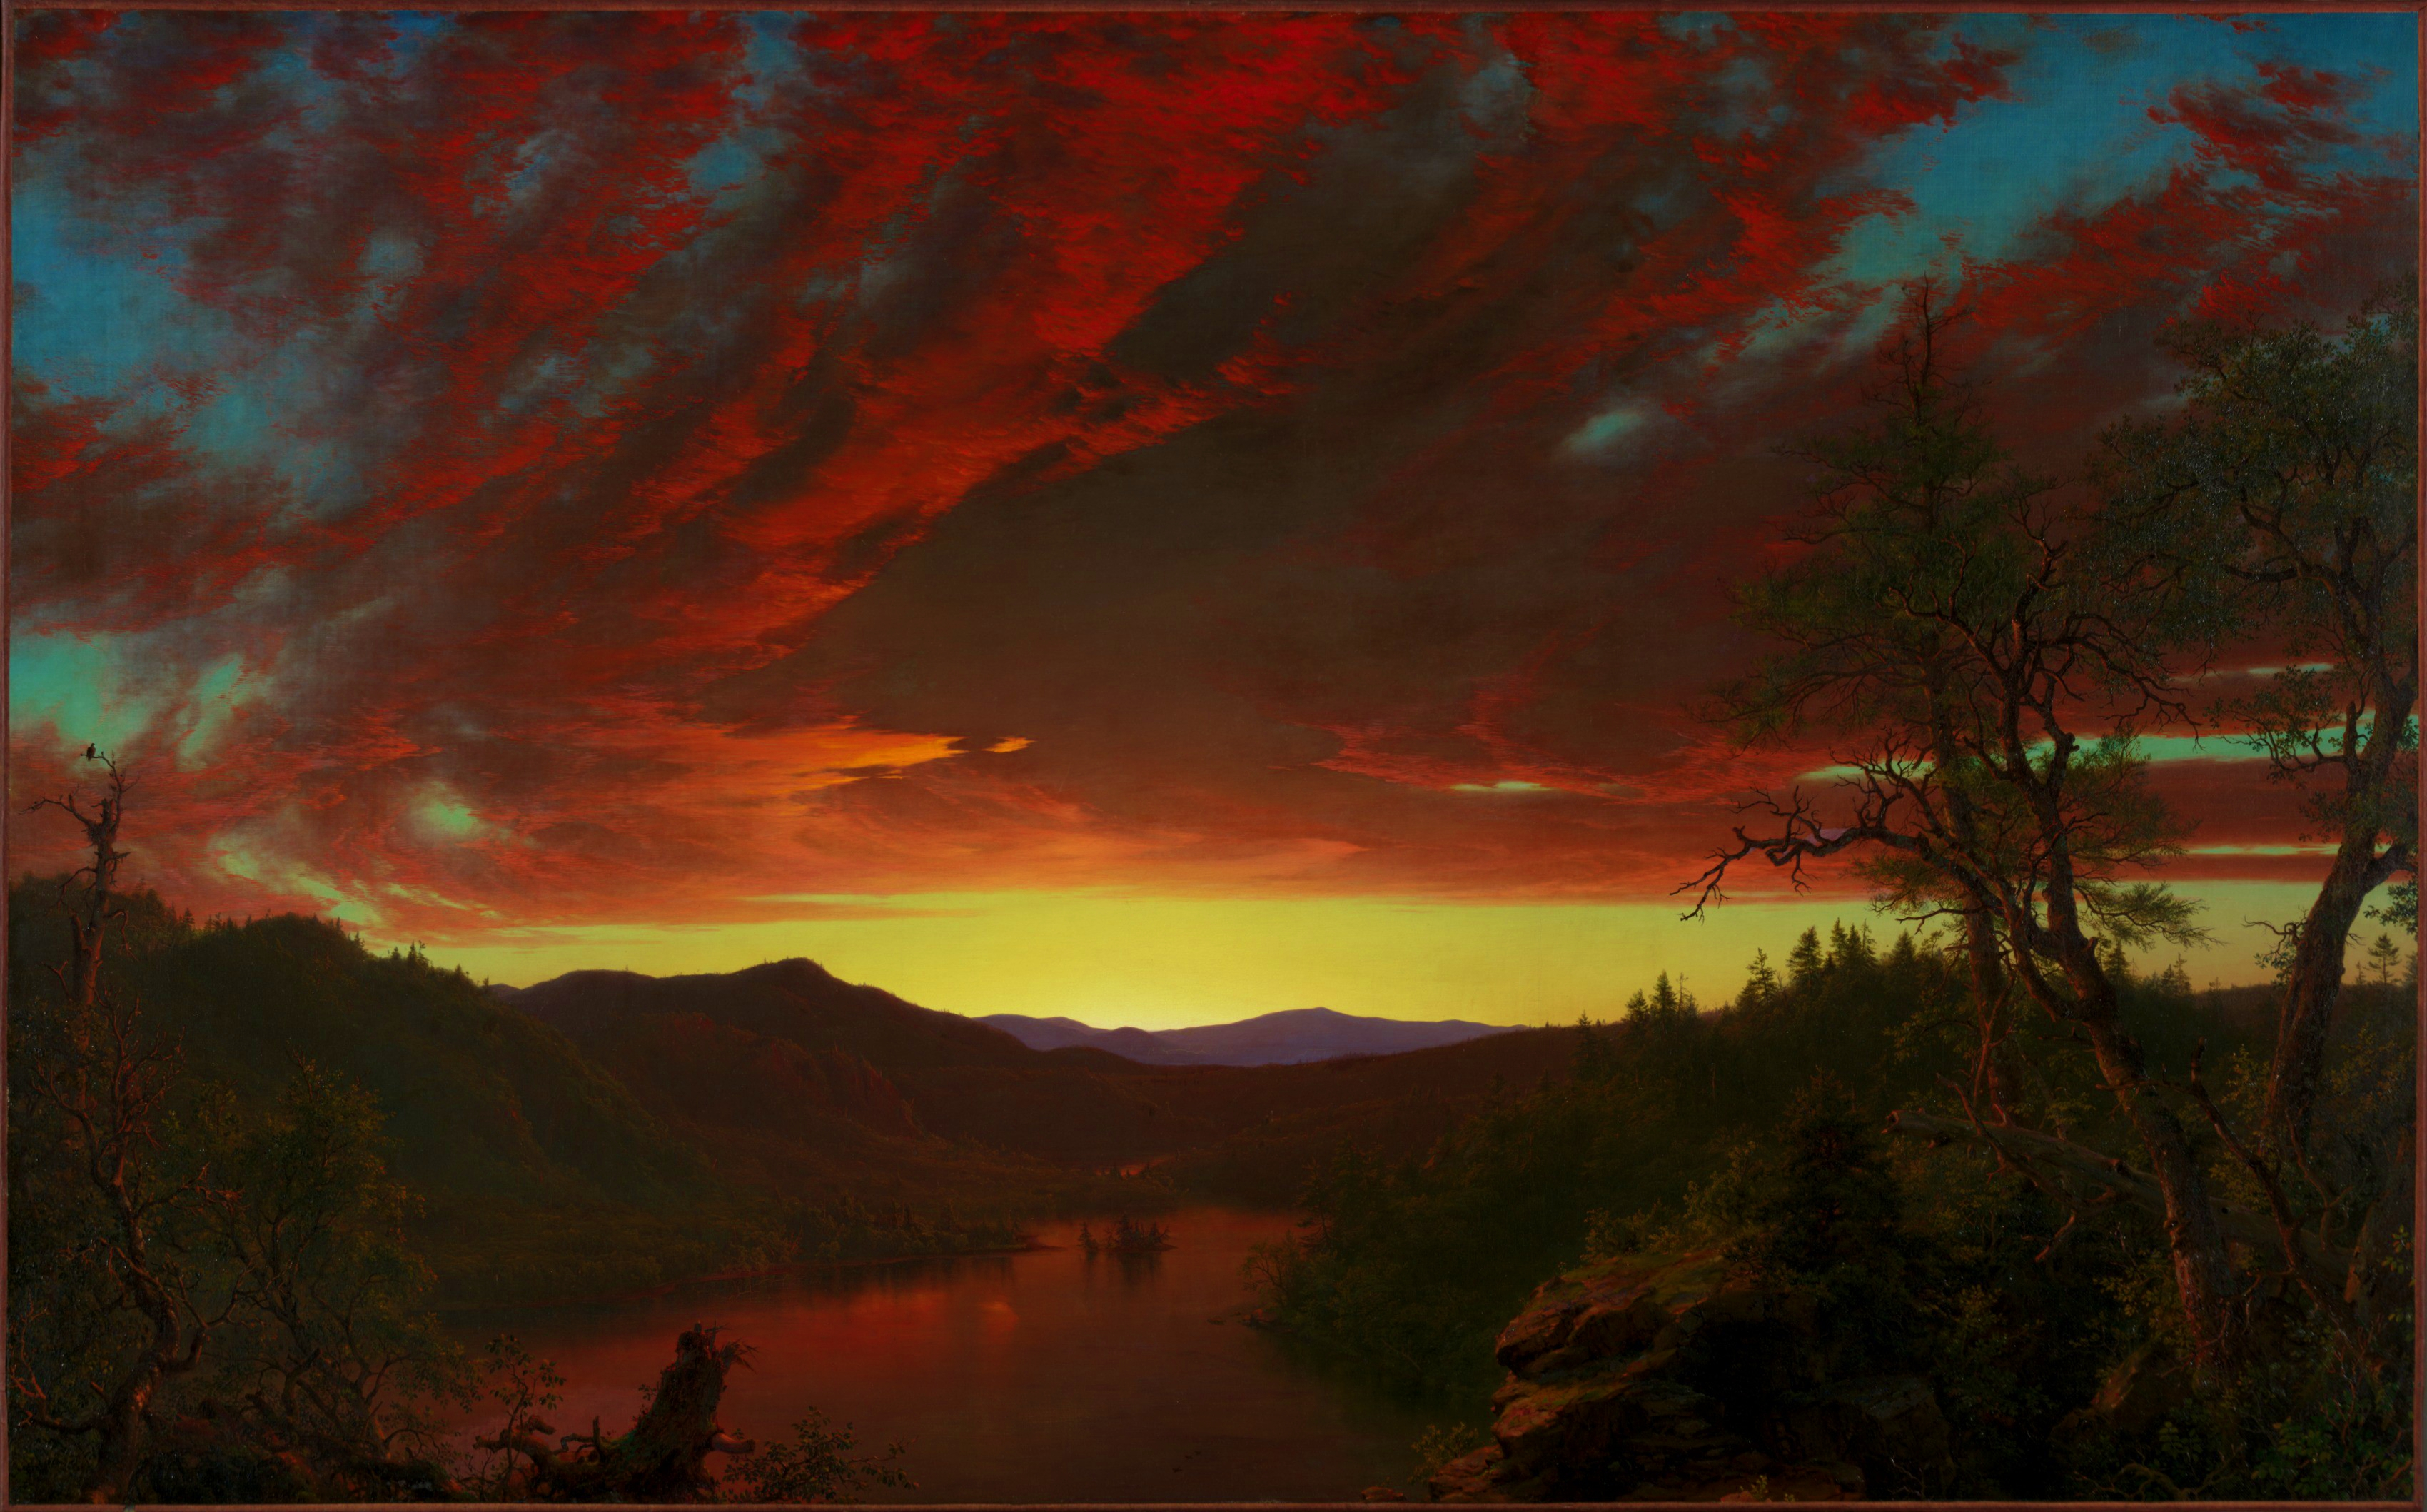
\includegraphics[width=1\textwidth]{report_src/effects/saturation_high.jpeg}
    \end{subfigure}
    \begin{subfigure}[b]{0.3\textwidth}
        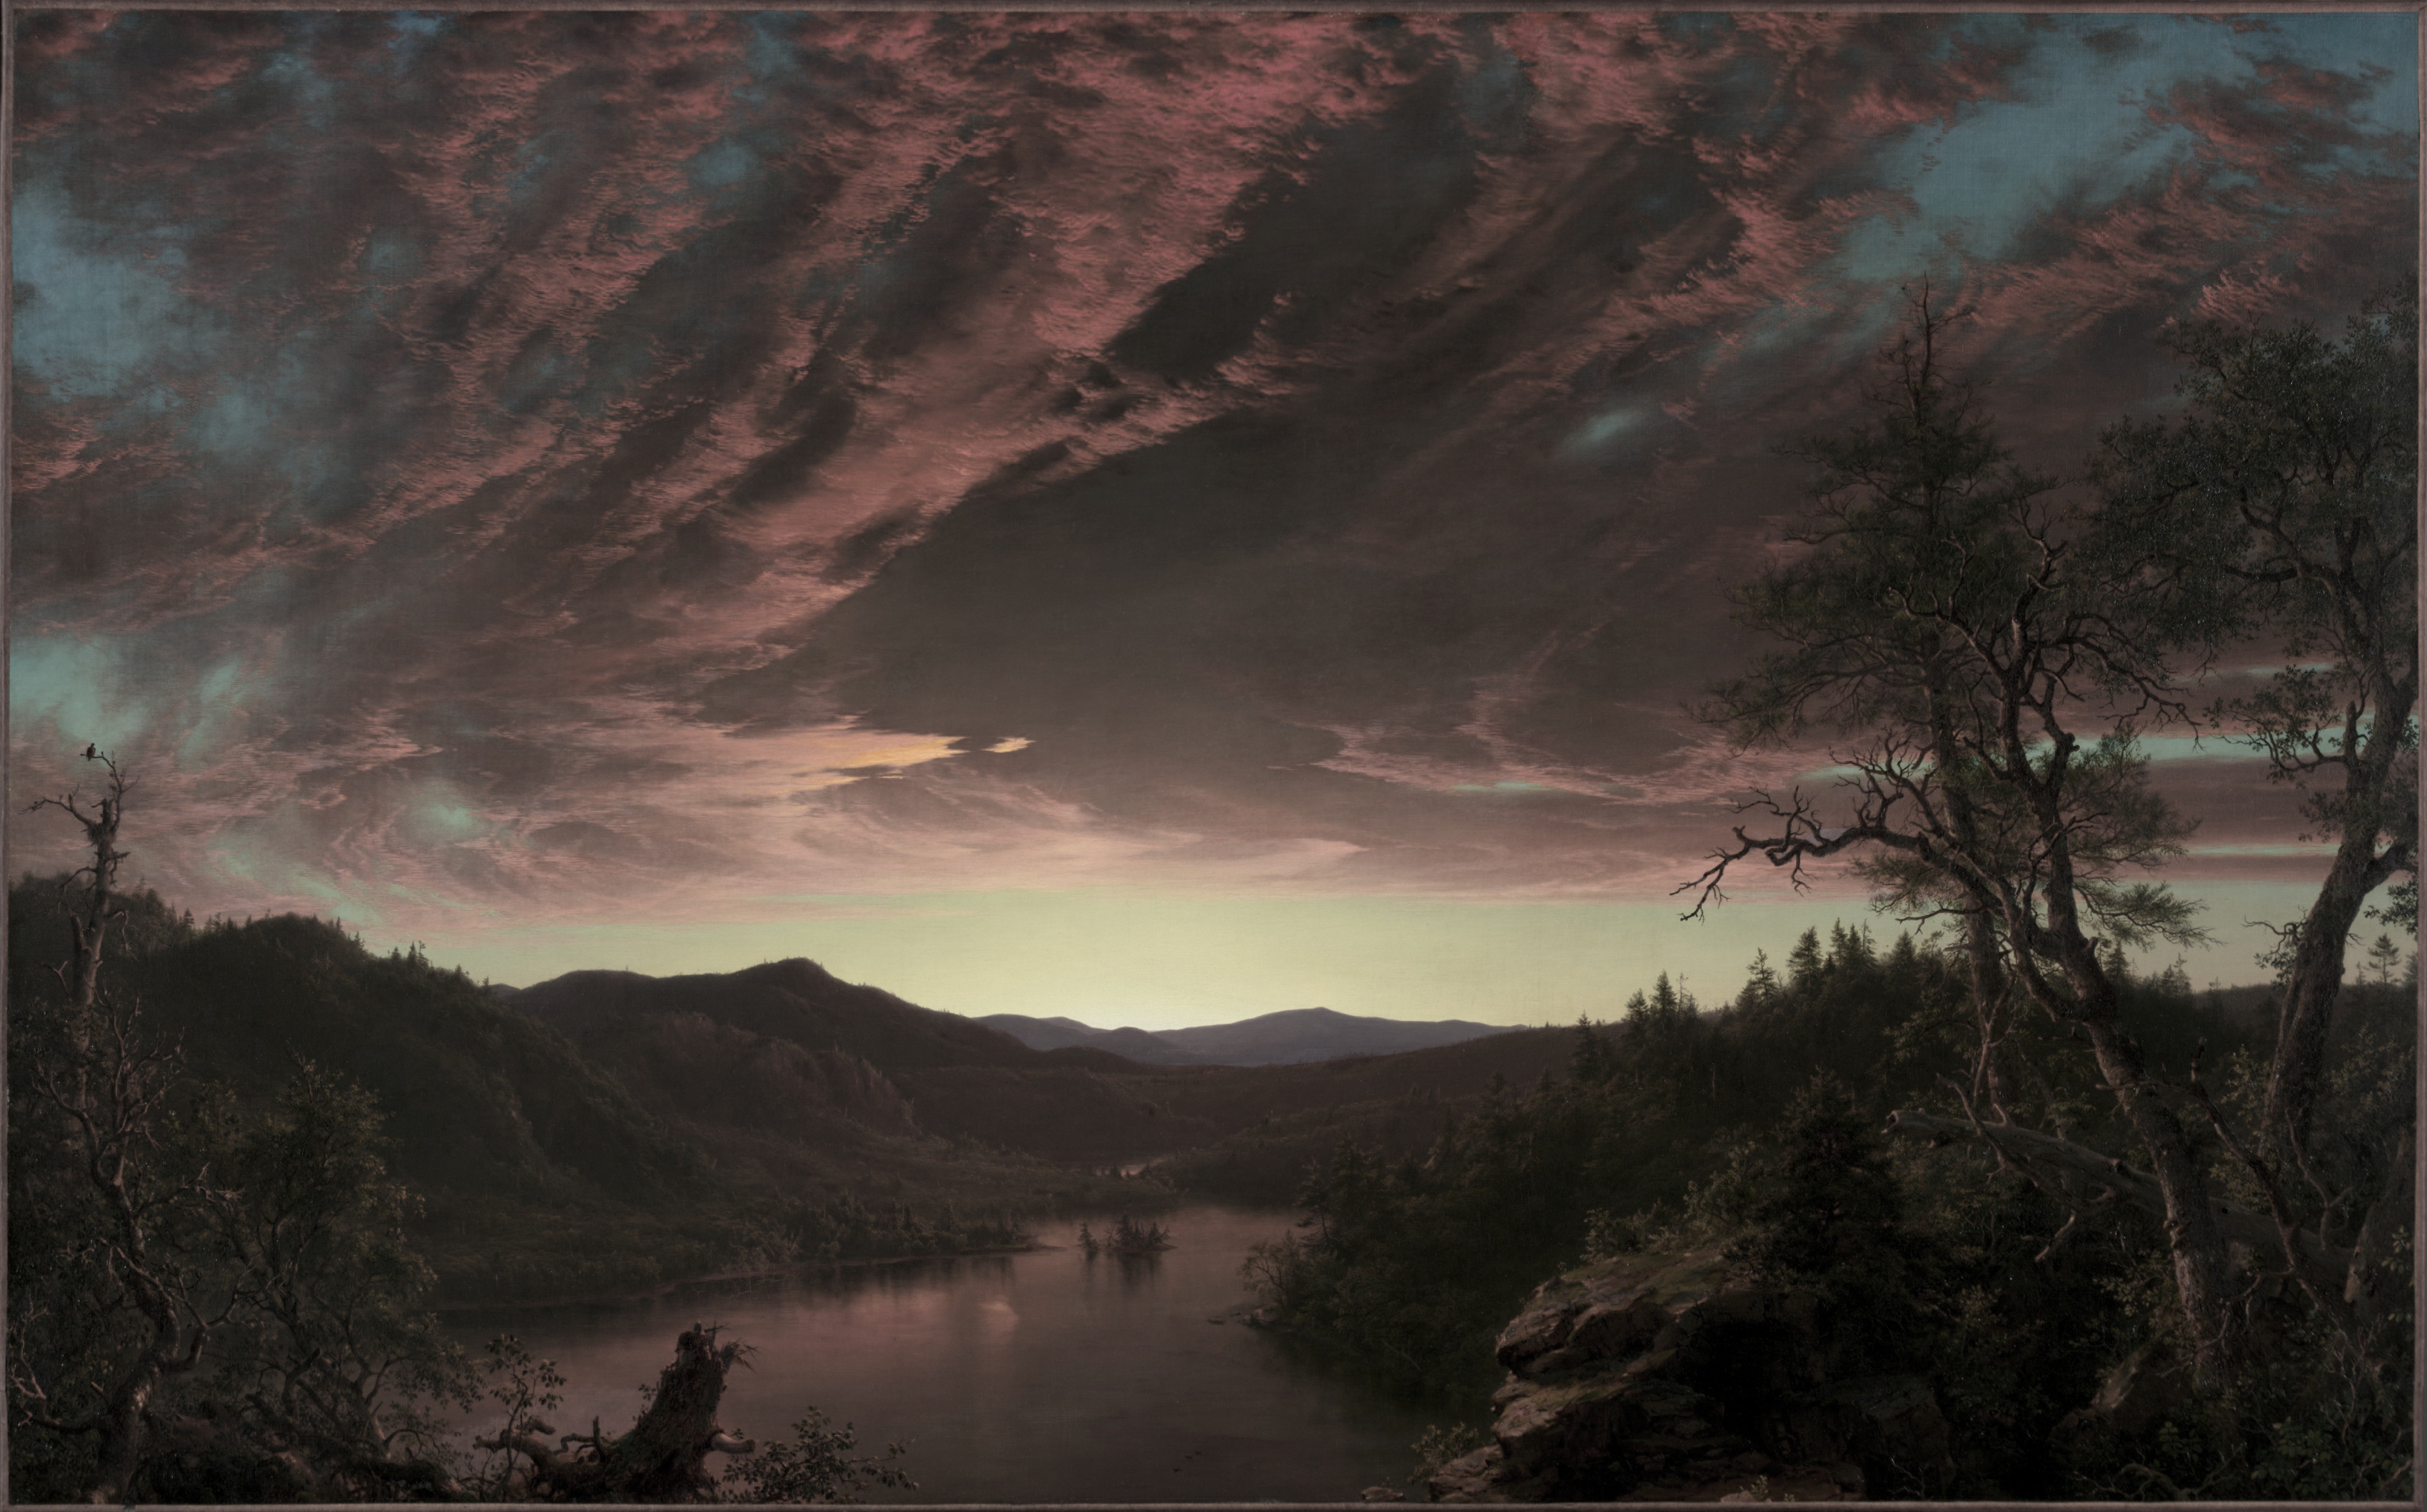
\includegraphics[width=1\textwidth]{report_src/effects/saturation_low.jpeg}
    \end{subfigure}
\end{figure} 

\emph{Méthode appelante : Retouching.setSaturation()}

\emph{Script : saturation.rs}
\\

Ce réglage permet de régler la saturation de l'image. Soit S la saturation existante, S' la nouvelle saturation et F le facteur de saturation. S et S' vont de 0 à 1.

On a S' = S + F * (1 - S) * S. 

On observe que la nouvelle saturation est proportionnelle à deux facteurs : l'espace restant avant une saturation totale (1-S) et la saturation existante S.
Par conséquent, en augmentant la saturation, chaque pixel tend vers sa saturation maximale, tout en garantissant une saturation proportionnelle à celle existante, évitant ainsi de saturer le gris.


\subsection{Egalisation d'histogramme (Enhance) :}

\begin{figure}[!h]
    \centering
    \begin{subfigure}[b]{0.3\textwidth}
        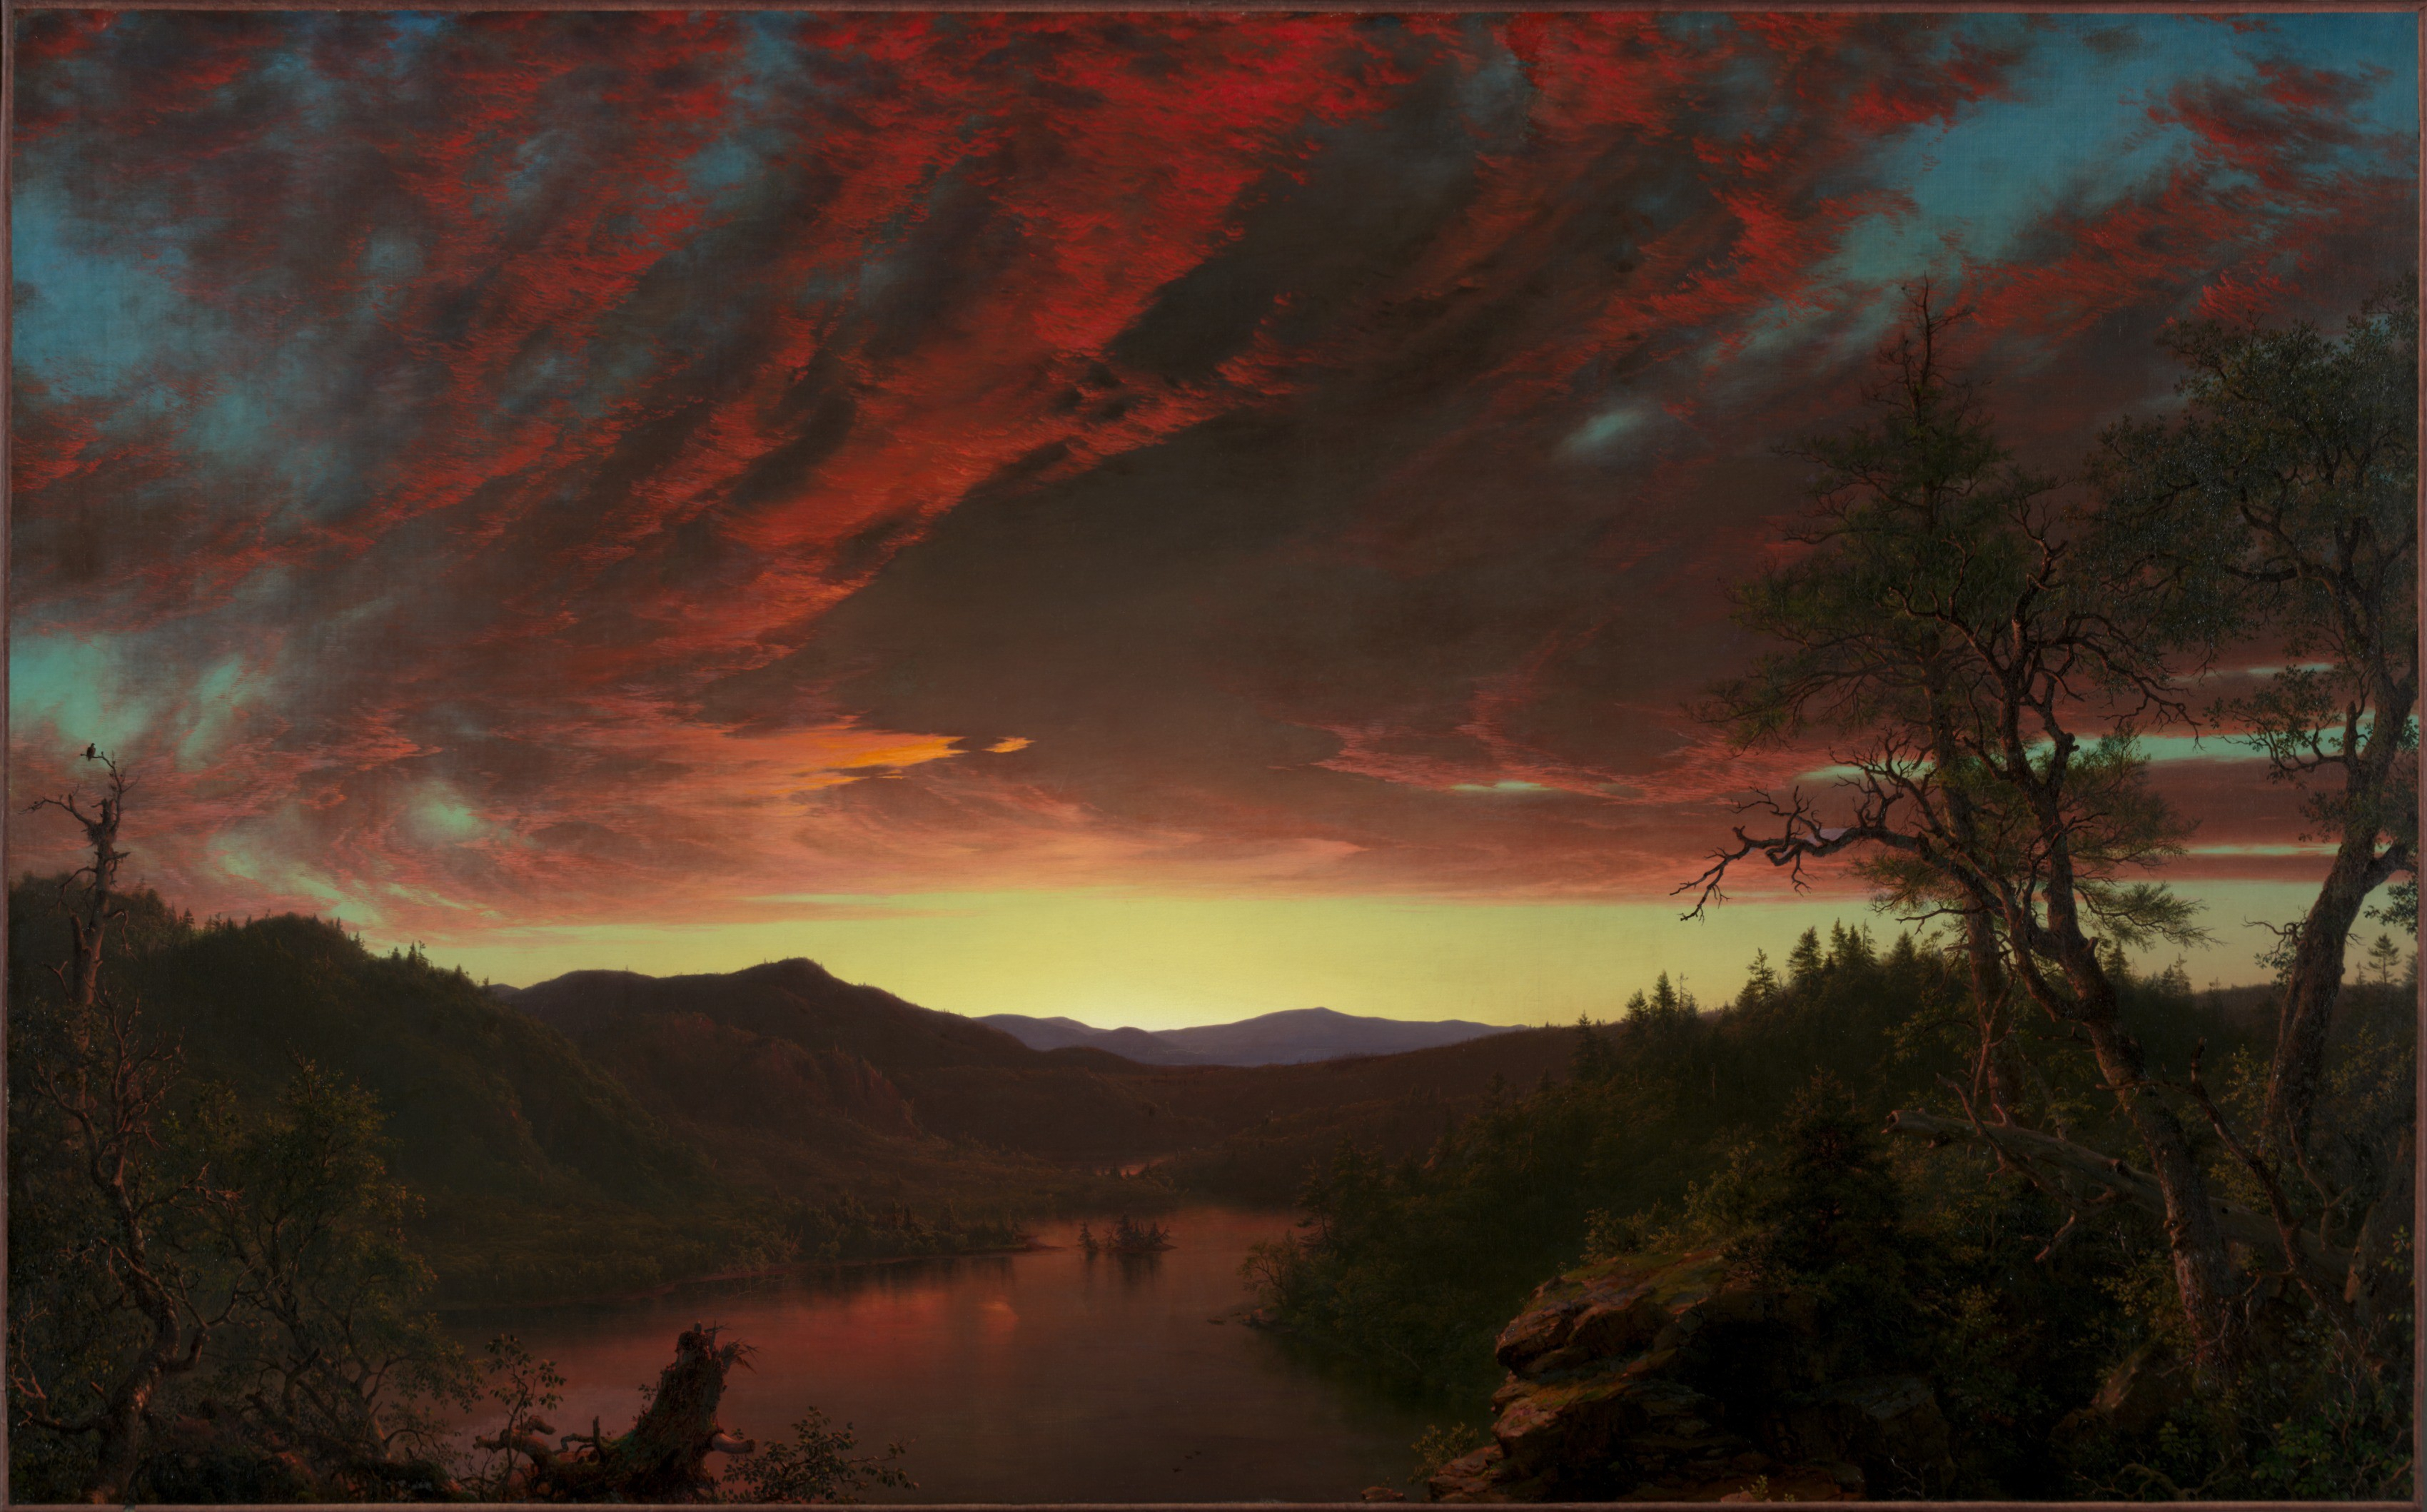
\includegraphics[width=1\textwidth]{report_src/effects/original1.jpeg}
    \end{subfigure}
    \begin{subfigure}[b]{0.3\textwidth}
        \includegraphics[width=1\textwidth]{report_src/effects/equalization.jpeg}
    \end{subfigure}
\end{figure} 

\emph{Méthode appelante : Retouching.histogramEqualization()}

\emph{Scripts : cumulativeHistogram.rs, assignLut.rs} 
\\

Comme son nom l'indique, cet effet utilise l'égalisation d'histogramme afin d'améliorer le contraste.
On calcule d'abord l'histogramme cumulé et on en déduit la LUT (Look Up Table), que nous assignons ensuite à chaque pixel.
\\

\subsection{Niveaux de gris (To gray) :}

\begin{figure}[!h]
    \centering
    \begin{subfigure}[b]{0.3\textwidth}
        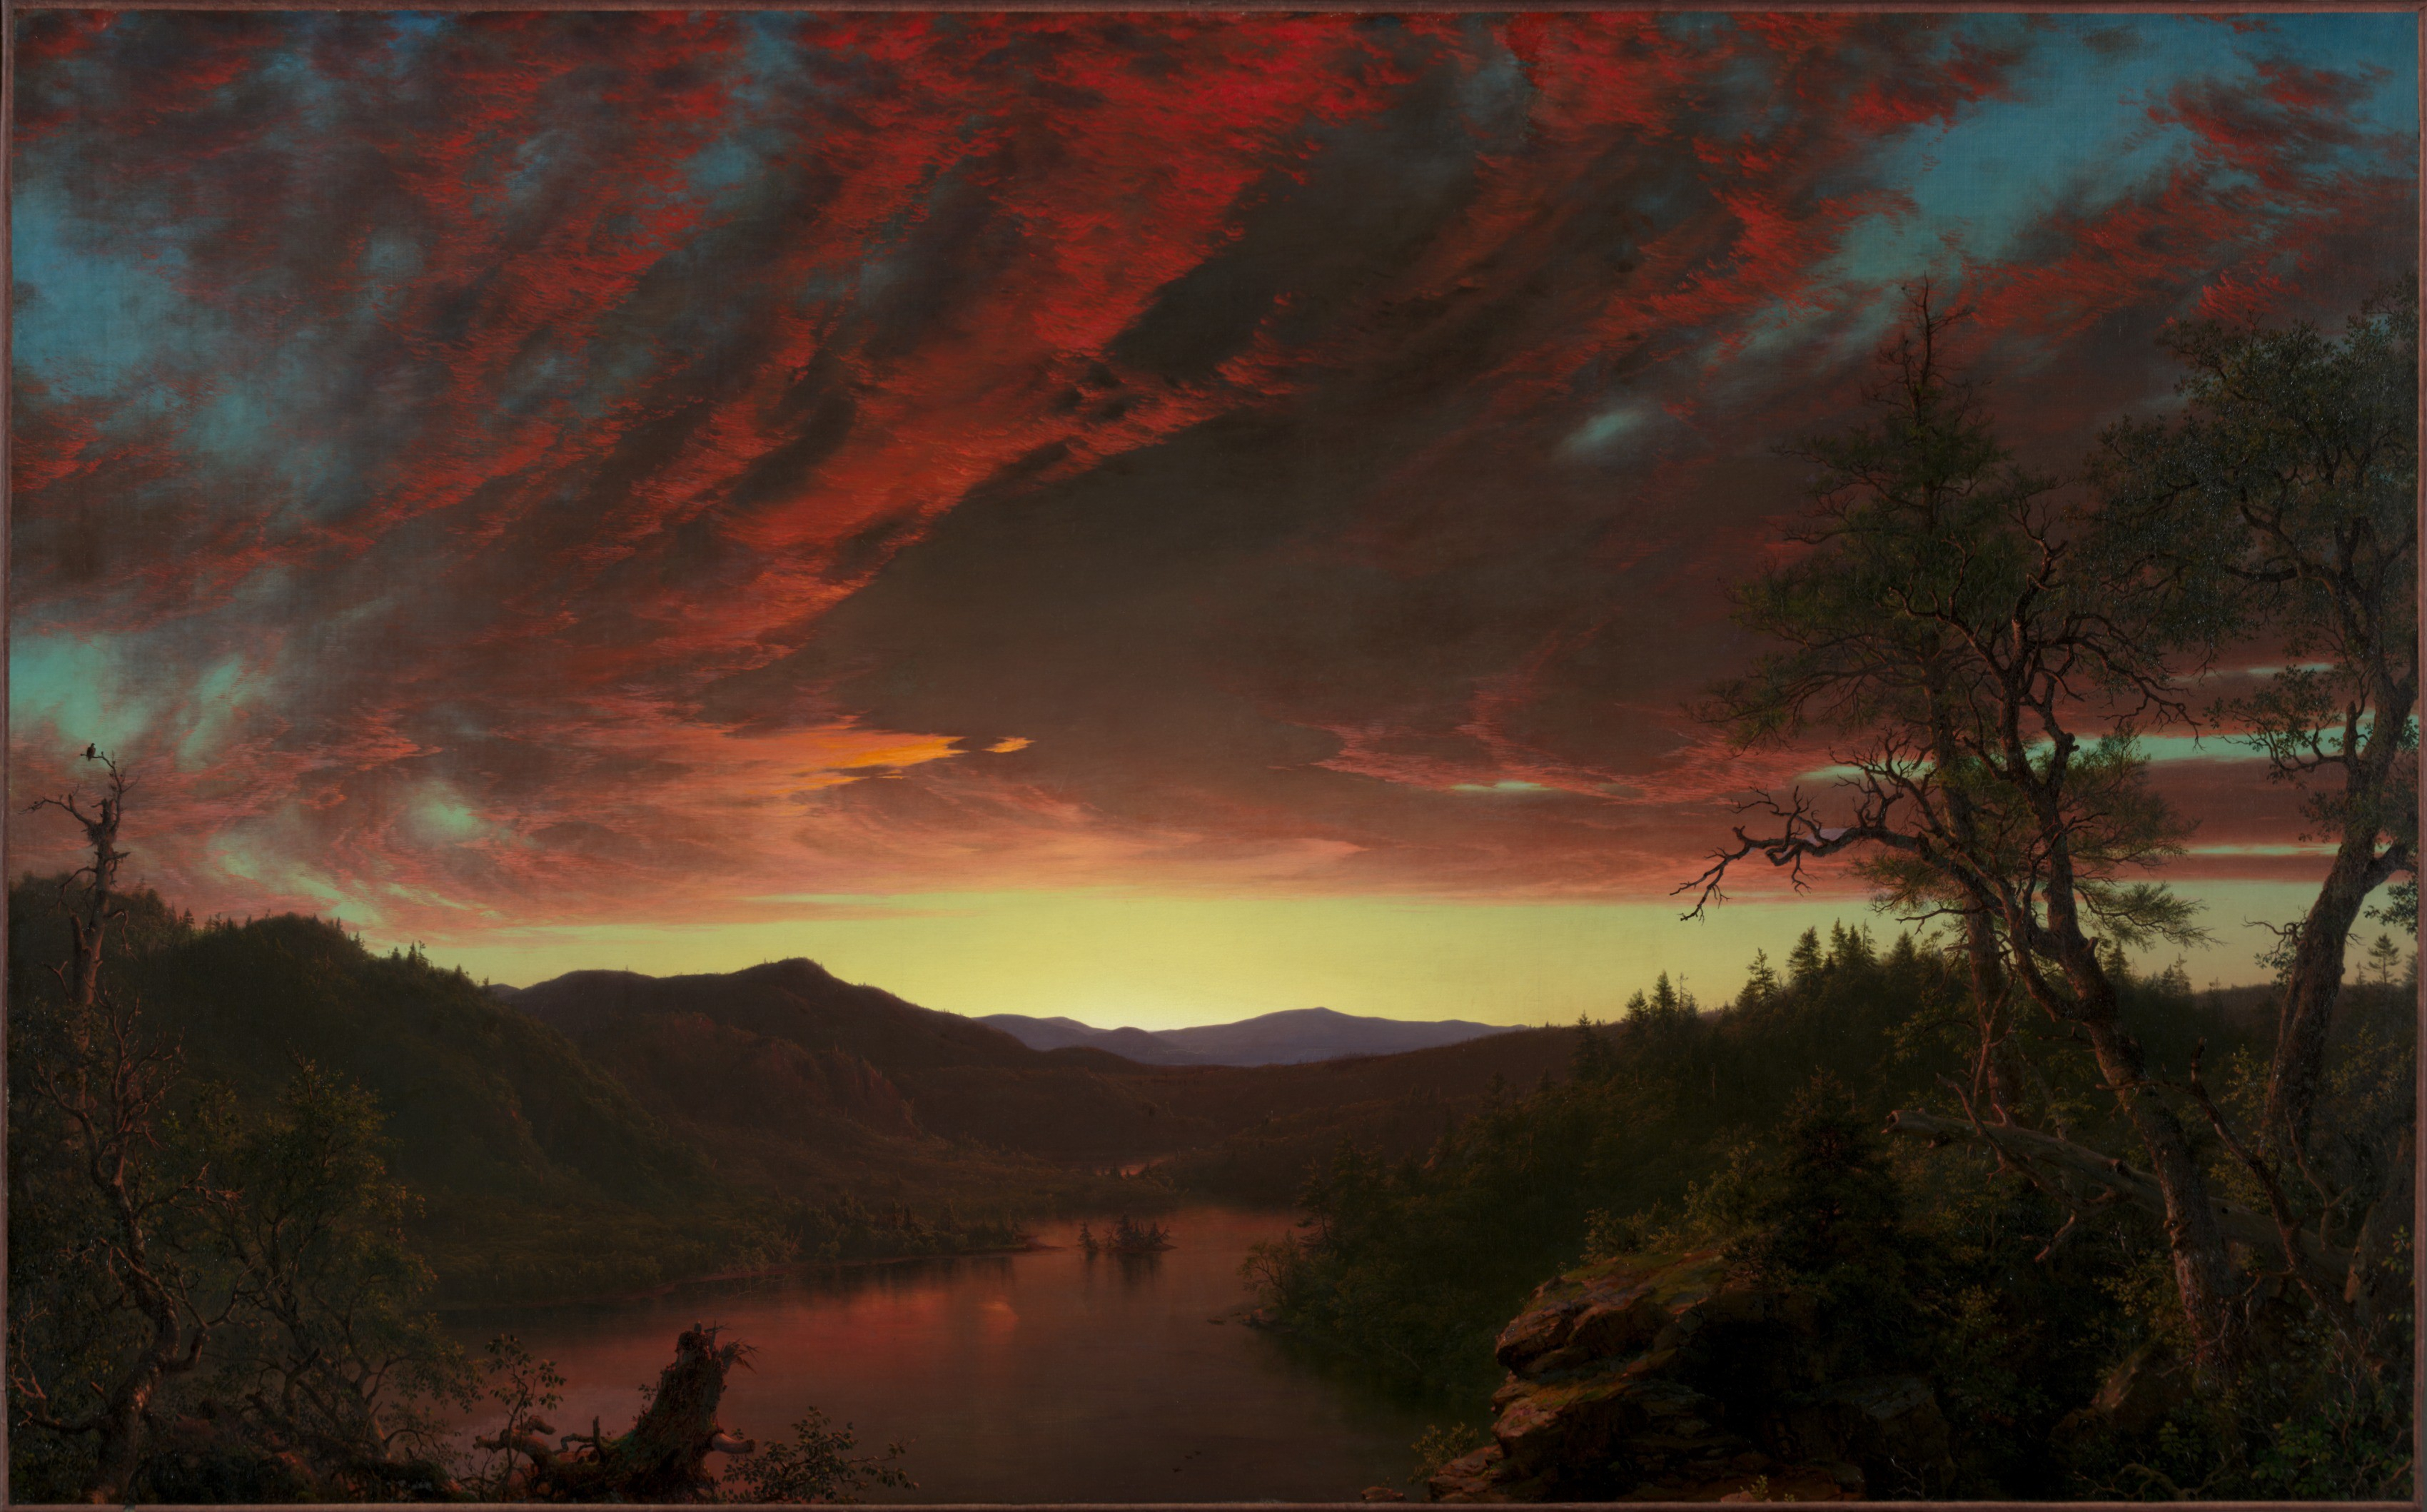
\includegraphics[width=1\textwidth]{report_src/effects/original1.jpeg}
    \end{subfigure}
    \begin{subfigure}[b]{0.3\textwidth}
        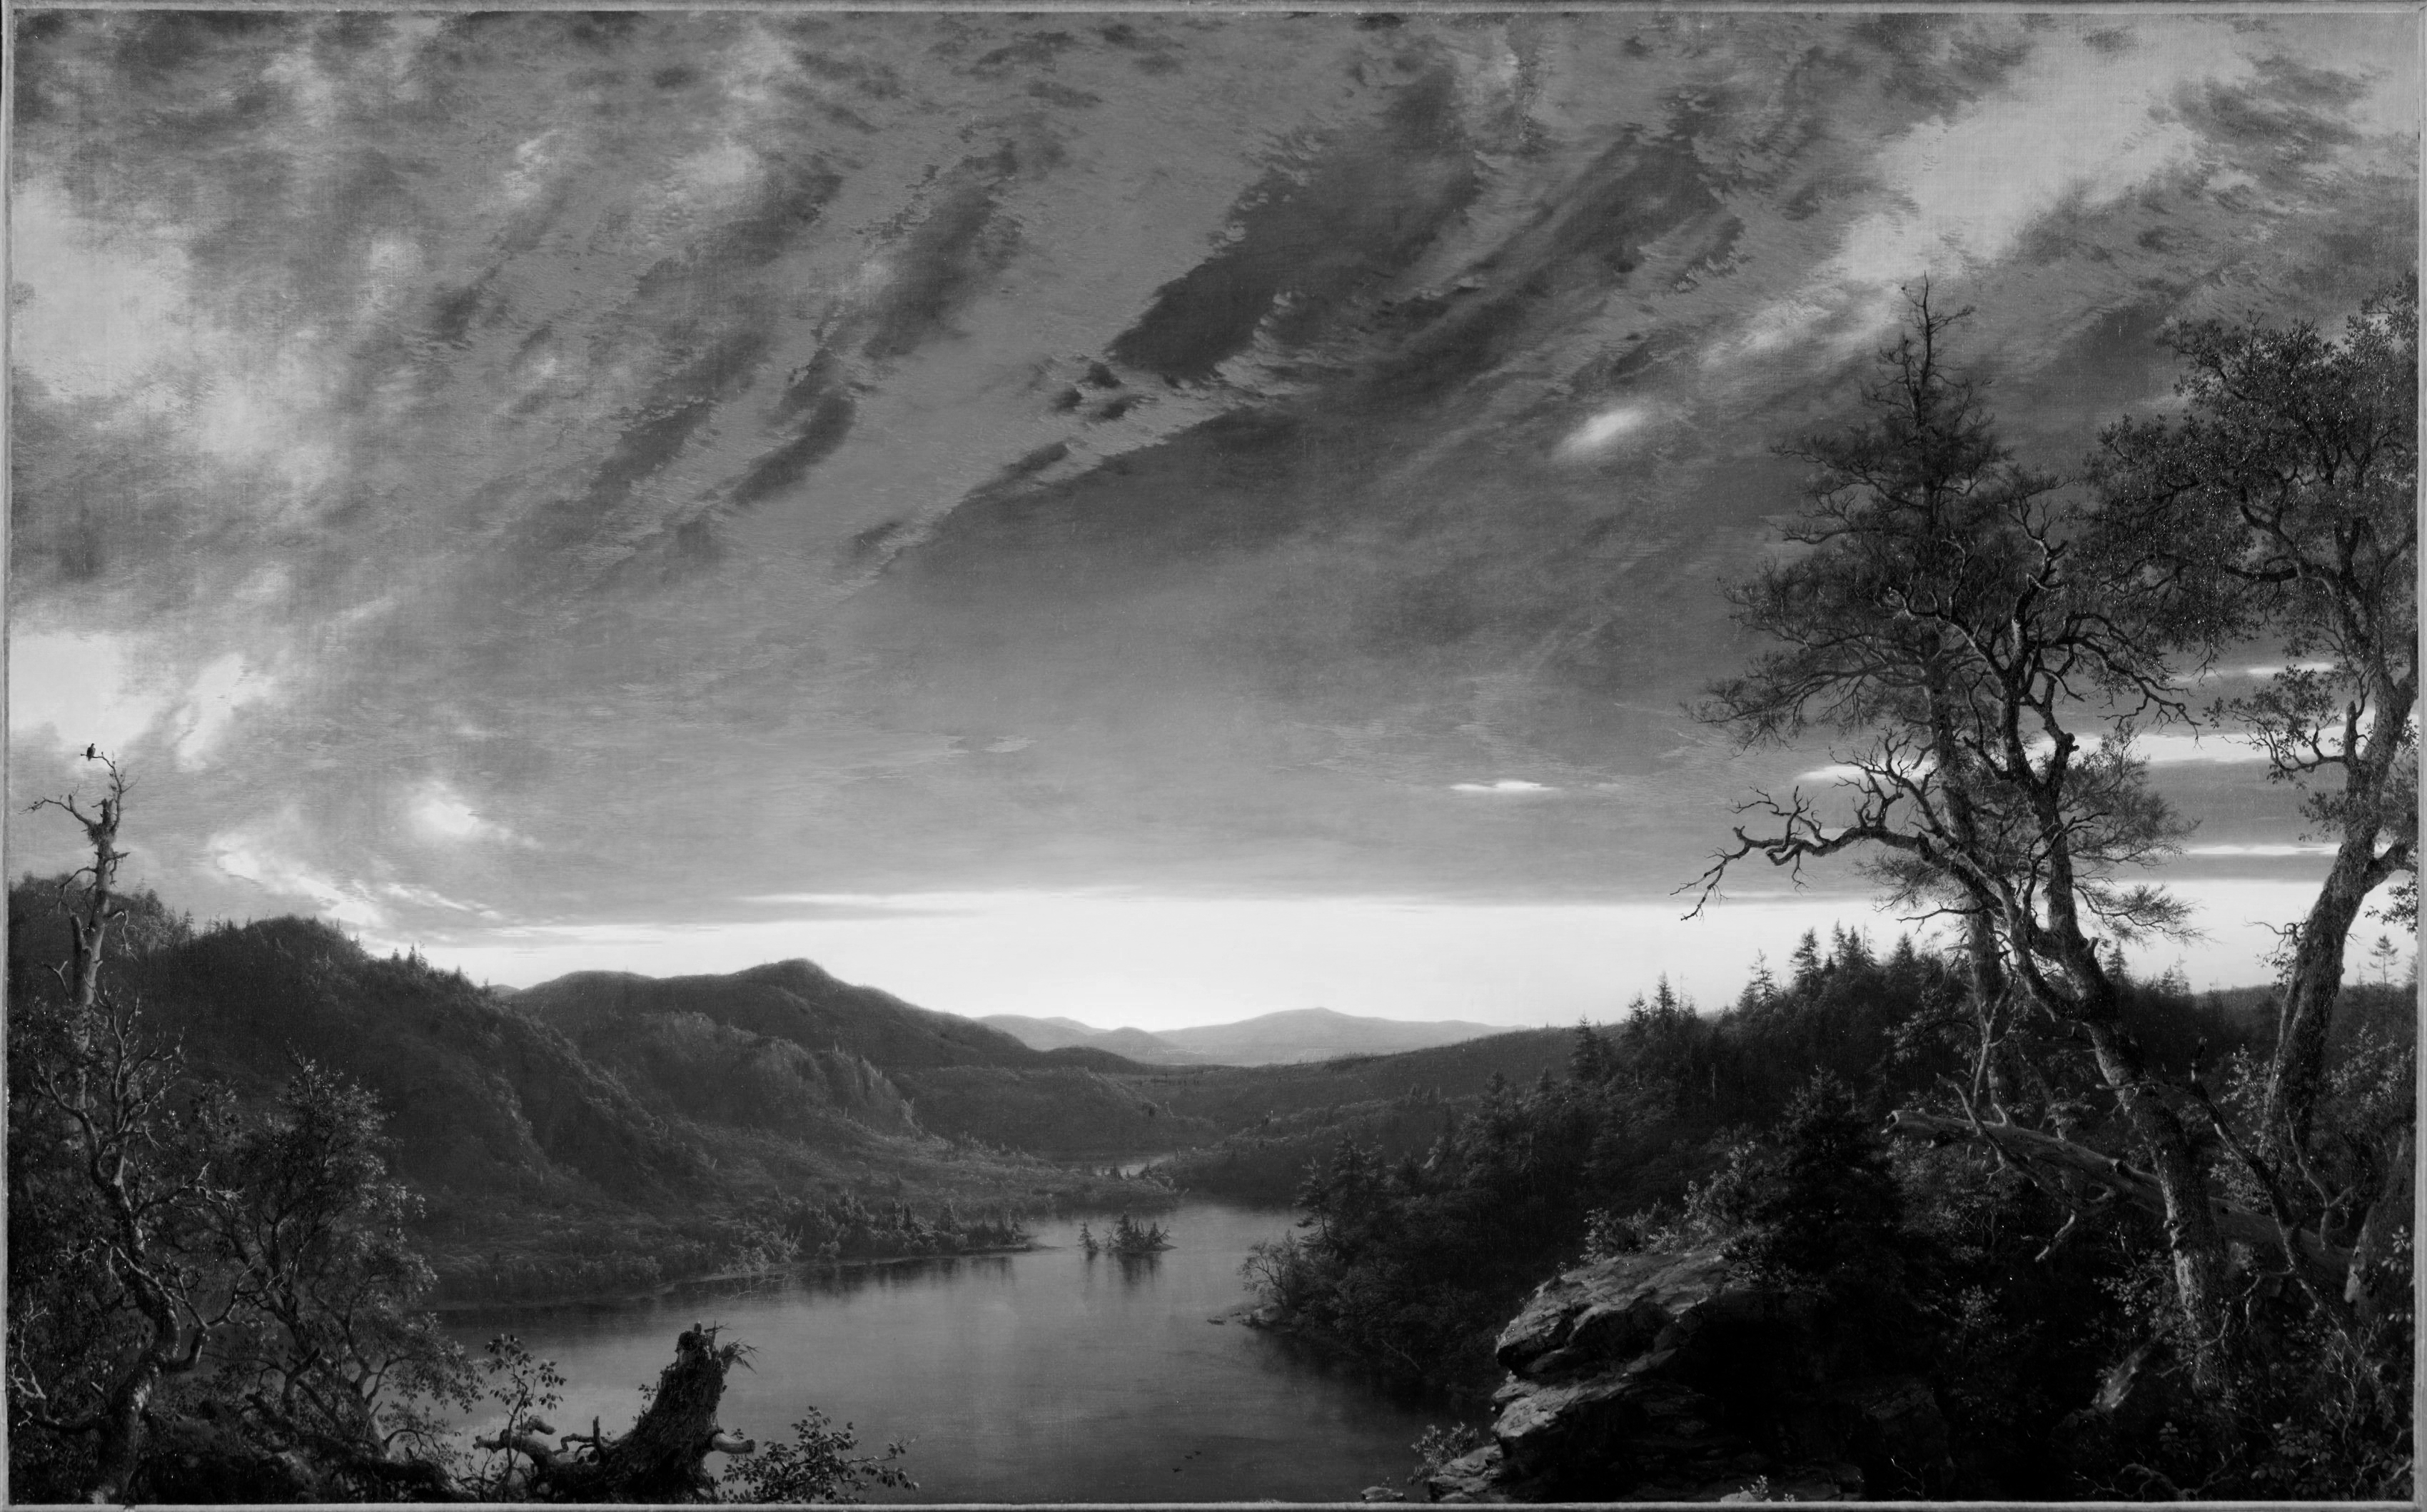
\includegraphics[width=1\textwidth]{report_src/effects/to_gray.jpeg}
    \end{subfigure}
\end{figure} 

\emph{Méthode appelante : Color.toGray()}

\emph{Scripts : utils.rs (méthode gray)} 
\\

Cet effet convertit une image en niveaux de gris. Pour chaque pixel, soit V la valeur du niveau de gris, R, G et B les trois canaux Rouge Vert Bleu de l'image, on applique :
\[            
    V =  R*0.299 + G*0.587 + B*0.114
\]

\subsection{Inverser (Invert) :}

\begin{figure}[!h]
    \centering
    \begin{subfigure}[b]{0.3\textwidth}
        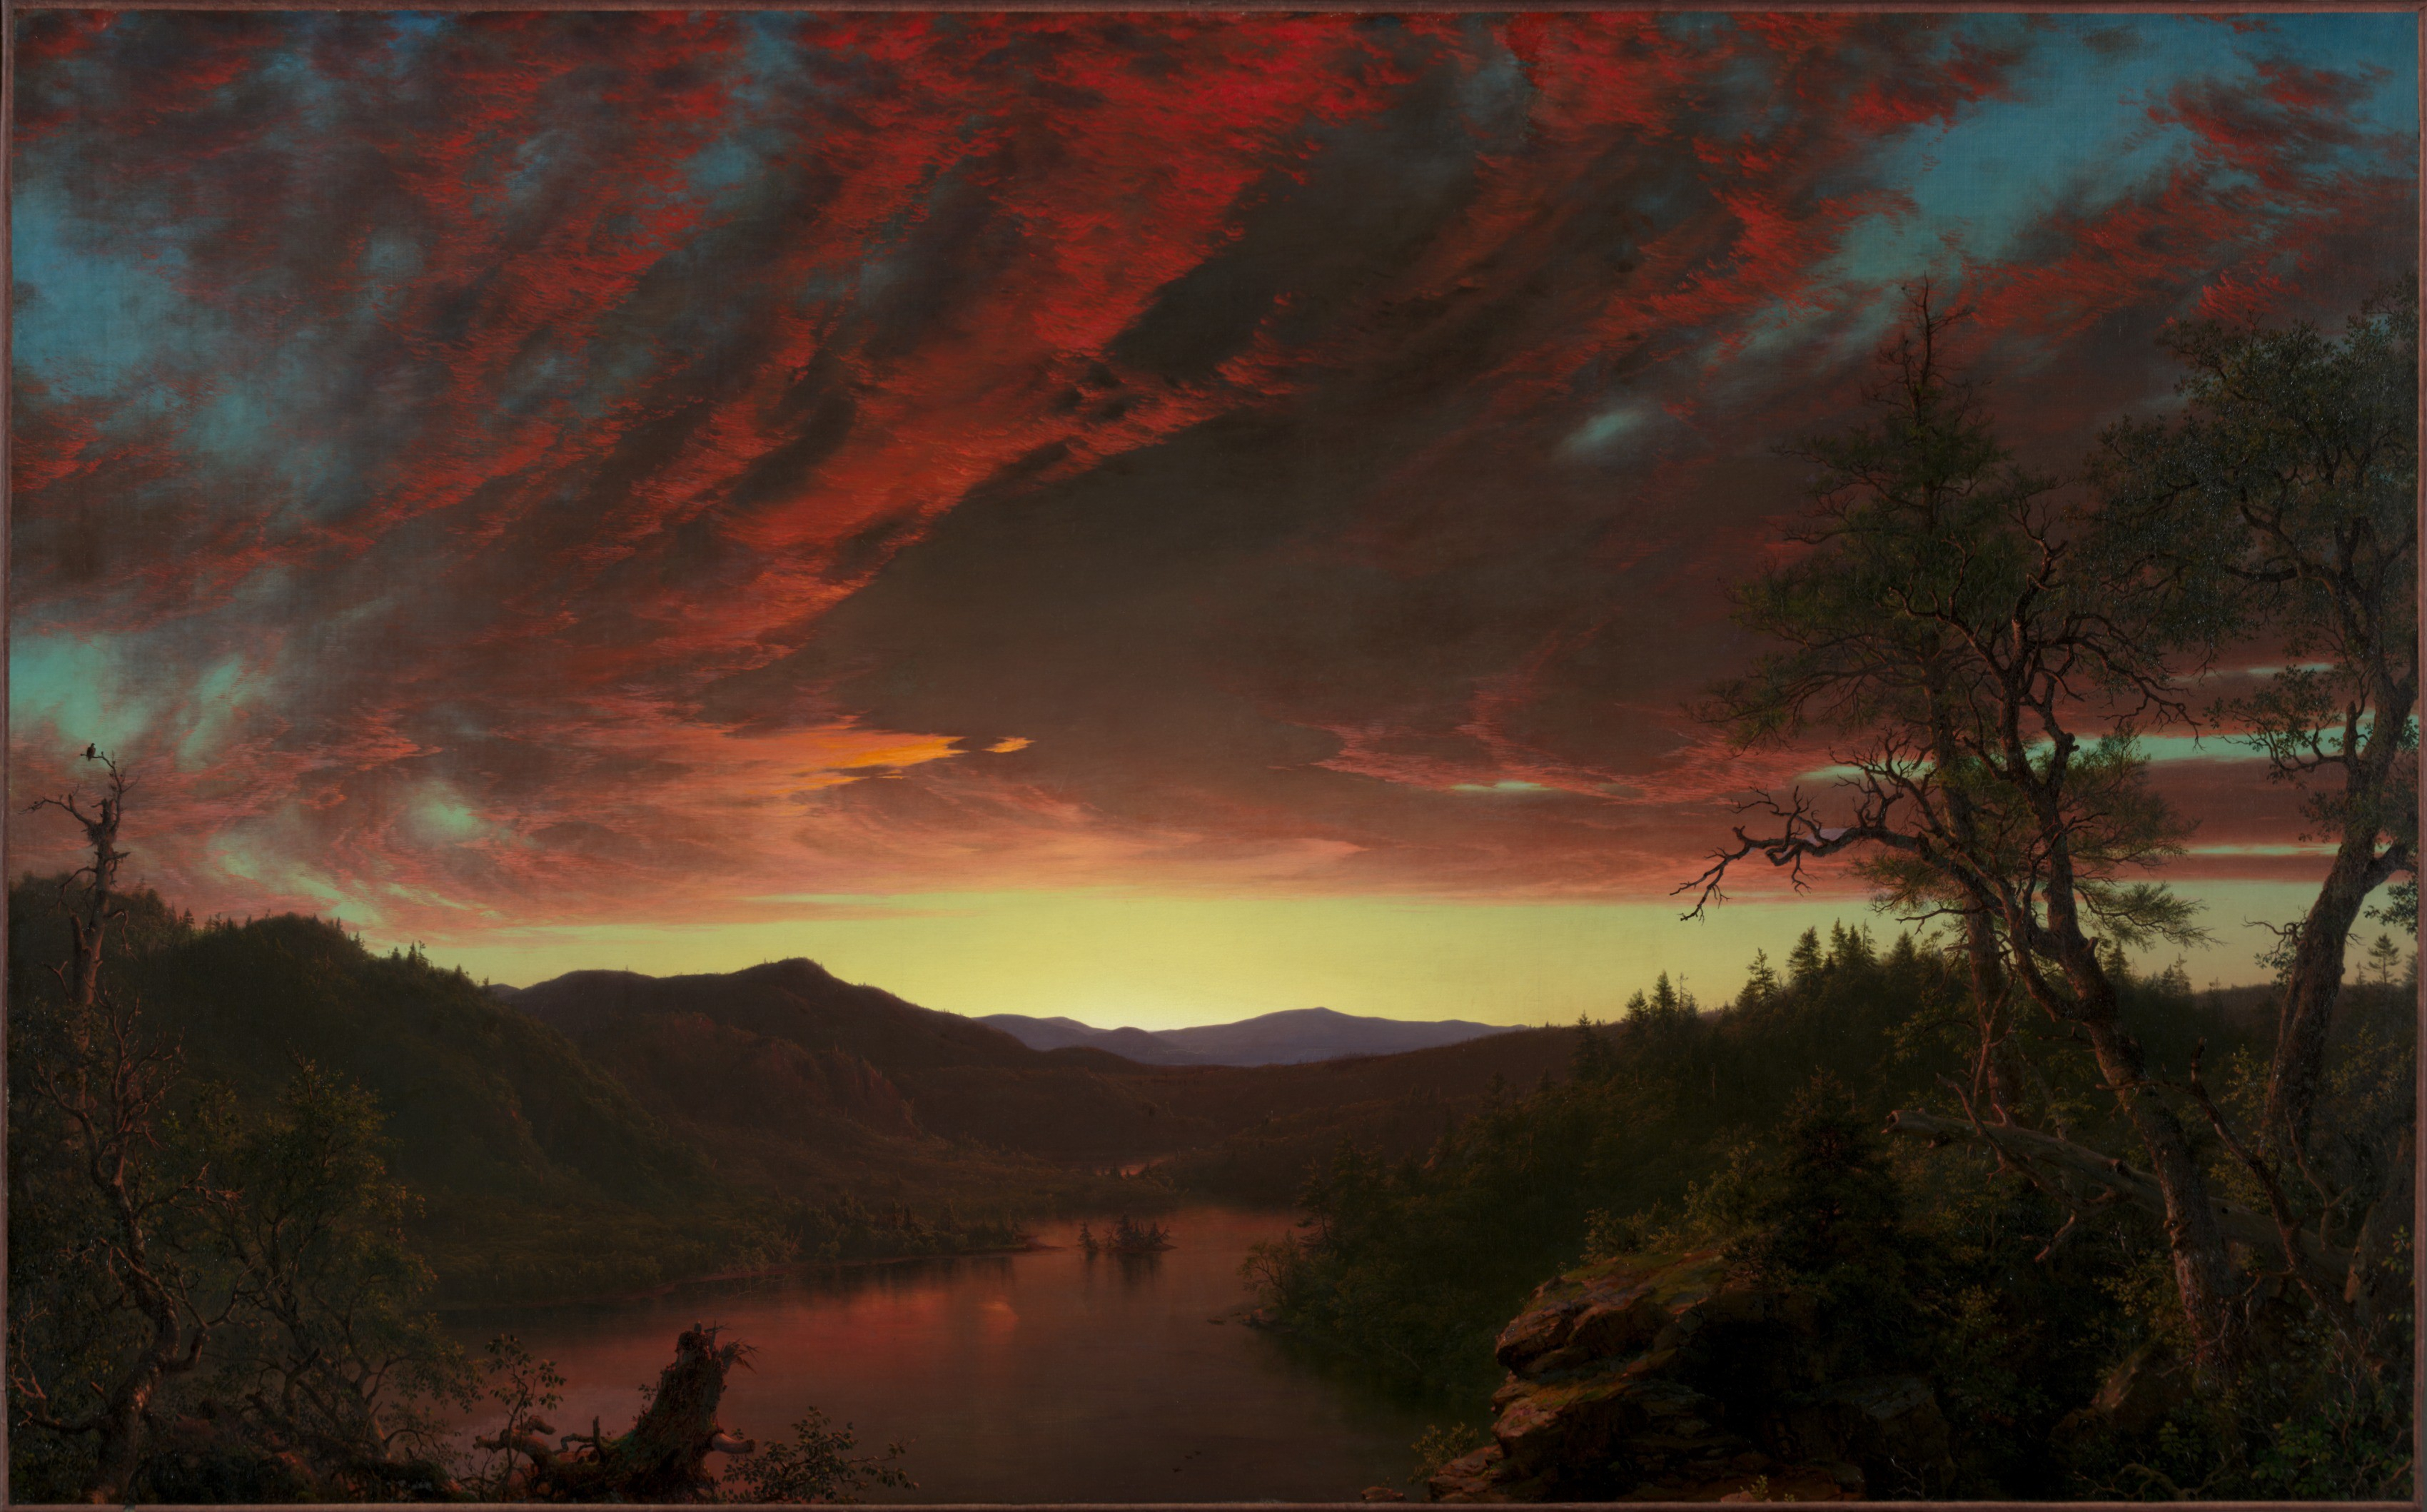
\includegraphics[width=1\textwidth]{report_src/effects/original1.jpeg}
    \end{subfigure}
    \begin{subfigure}[b]{0.3\textwidth}
        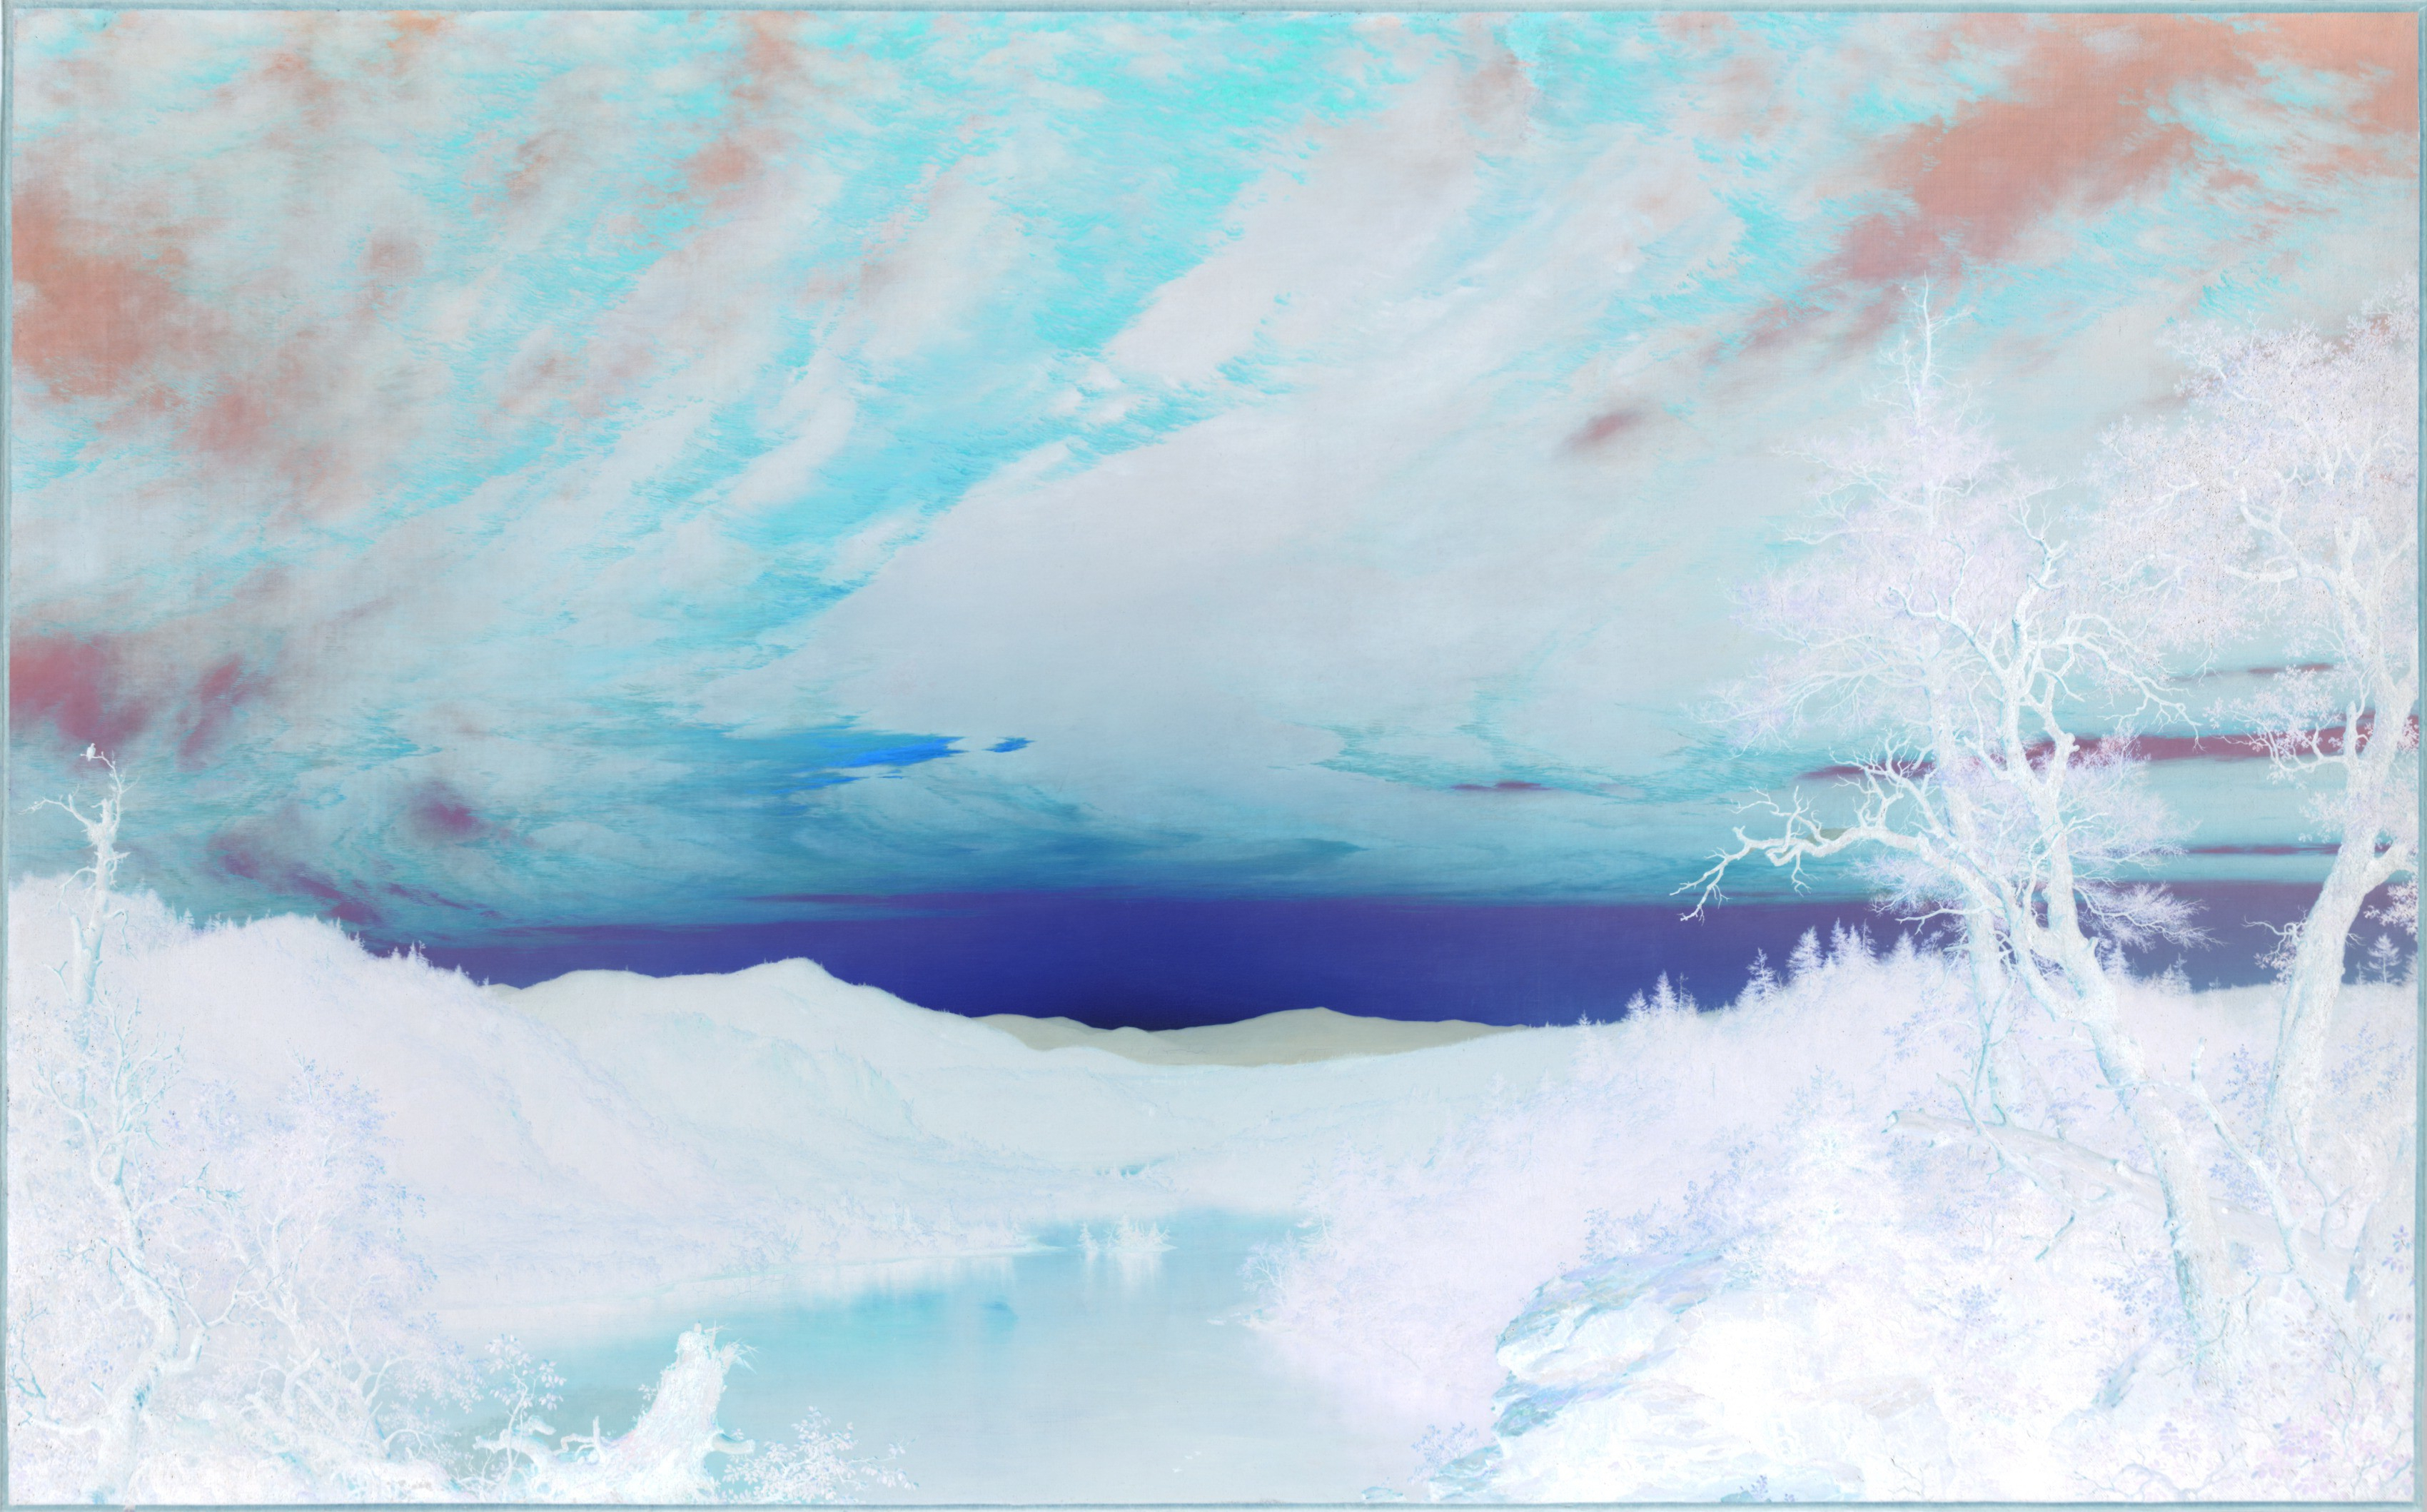
\includegraphics[width=1\textwidth]{report_src/effects/invert.jpeg}
    \end{subfigure}
\end{figure} 

\emph{Méthode appelante : Color.invert()}

\emph{Scripts : utils.rs (méthode invert)} 
\\

Cet effet inverse les couleurs d'une image. Pour chaque pixel, soit R, G et B les canaux Rouge Vert Bleu de l'image et R' G' B' les nouvelles couleurs, on a :

\[            
    R' =  255 - R
\] 
\[            
    G' =  255 - G
\]  
\[            
    B' =  255 - B
\] 


\subsection{Hue :}

    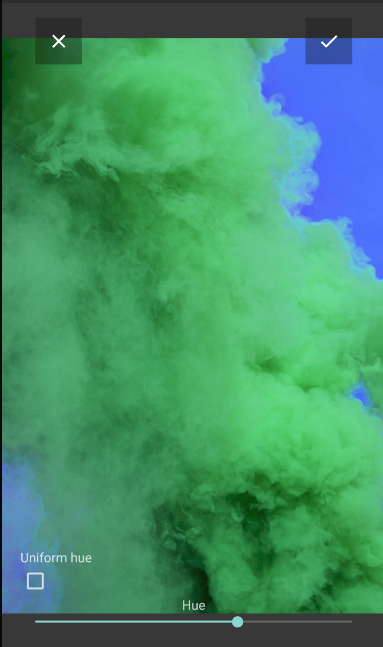
\includegraphics[width=0.25\textwidth]{report_src/effects/non-uniform-hue.png}
    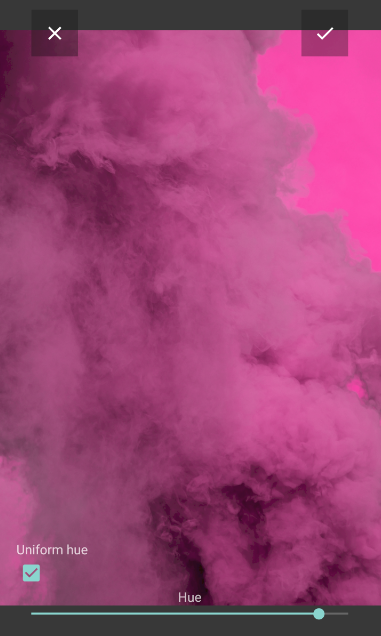
\includegraphics[width=0.25\textwidth]{report_src/effects/uniform-hue.png}
    \newline
    \emph{Méthode appelante : Color.colorize()}
    \emph{Scripts : colorize.rs, utils.rs} 
    \newline

    Ce reglage efectue une conversion des couleurs de chaque pixel du format RGB au HSV puis change le champ Hue du pixel ce qui permet de 
    changer la teinte de image.
    La teinte en question est sélectionné par l'utilisateur grâce a la seekbar qui lui est fournie ainsi qu'une option a cocher qui lui propose deux choix:
    \\

    \emph{Teinte uniforme:}
        En cochant la case "uniforme" l'effet remplace le teinte de tout les pixels de l'image en changeant le champ hue de chaque pixel par celui choisis par l'utilisateur grâce à la seekbar.
        

    \emph{Teinte non uniforme:}
        En décochant la case "uniforme" ajoute le teinte sélectionné par l'utilisateur grâce à la seekbar au chanp hue déjà contenu dans chaque pixel donnant un nouveau 
        teinte a chaque couleur de l'image.
        


\subsection{Keep hue :}

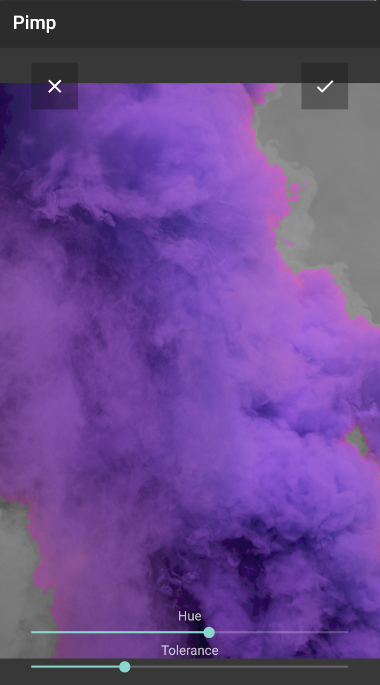
\includegraphics[width=0.25\textwidth]{report_src/effects/keepColor.png}
\newline
\emph{Méthode appelante : Color.keepColor()}
\emph{Scripts : keepColor.rs, utils.rs} 
\newline

Garde qu'une seul teinte avec un degré de tolérance sélectionné par l'utilisateur grâce aux deux seekbars "hue"  et "tolerance" qui lui sont fournies et garde 
le reste des pixels en échelle de gris en convertissant les couleurs de chaque pixel du format RGB au HSV puis gardant que les pixel contenant le hue choisi dans le bon intervalle.
\\

\subsection{Convolution (Blur, Sharpen, Neon) :} \label{convolution}

    Dans cette sous-section on retrouve des effets réalisés avec des convolutions pour flouter une image en passant par deux types différents de kernel : Gaussien et moyenneur
    (bouton "Blur"), des effets pour améliorer la netteté d'une image avec la fonction "Laplacian of gaussian" (bouton Sharpen) et des effets de 
    détection de contours (bouton "Neon") en réalisant des convolutions avec des opérateurs comme Sobel, Prewitt, Kirsch ou une convolution simple avec un kernel
    laplacien.
    \\

    Pour ces effets nous avons implémenté 3 méthodes de convolution.


    \begin{itemize}
        \item Convolution classique.
        \item Convolution séparable.
        \item Convolution détection de contours.
    \end{itemize}
    

    \subsubsection*{Convolution classique} \label{conv_classique}
    
        Cette méthode de convolution suit le même algorithme vu en cours, on peut l'appliquer avec des noyaux asymétriques de dimensions impaires uniquement,
        cette opération a été parallélisée grâce à \textbf{renderscript} qui parallélise le calcul par CPU multithreading/GPU. En plus, dans cette méthode (et dans toutes les autres) nous avons rajouté
        des optimisations pour parcourir seulement les index nécessaires de l'image lors de la convolution. En calculant les index des centres des deux dimensions du kernel
        on peut anticiper et éviter les appels de fonction inutiles sur les bords de l'image par exemple.
        
        $X_{d\acute{e}but}$ et $X{fin}$ étant le premier et dernier index à parcourir dans l'axe des abscisses respectivement et
        $Y_{d\acute{e}but}$ et $Y_{fin}$ étant le premier et dernier index à parcourir dans l'axe des ordonnées respectivement.
        \[
            Kernel_{CentreX} =   \frac{Largeur_{kernel}}{2}            
        \]
        \[
            Kernel_{CentreY} =   \frac{Hauteur_{kernel}}{2}            
        \]
        \[
            X_{d\acute{e}but} = Kernel_{CentreX}      
        \]
        \[
            X_{fin} = Largeur_{image} - Kernel_{CentreX}           
        \]
        \[
            Y_{d\acute{e}but} = Kernel_{CentreY}      
        \]
        \[
            Y_{fin} = Hauteur_{image} - Kernel_{CentreY}           
        \]

        En définissant les index du début et de fin de parcours pour les deux dimensions de l'image sur le script de lancement renderscript
        comme ci-dessus on peut se passer de quelques appels de fonctions sur les bords de l'image et ainsi gagner du temps de calcul.

    \subsubsection*{Convolution séparable} \label{conv_separable}

        Pour la convolution classique avec un kernel de taille $N*M$ on doit faire $N*M$ multiplications pour chaque échantillon,
        cependant si le kernel est séparable on peut passer à $N+M$ opérations. Voir \ref{separable_source}.
        \\

        Or, afin d'optimiser le calcul de la convolution sur des filtres séparables comme le filtre gaussien et moyenneur, nous avons implémenté une
        méthode de convolution séparable.
        
        \begin{figure}[!h]
            \centering
            \begin{subfigure}[b]{1\textwidth}
                \centering
                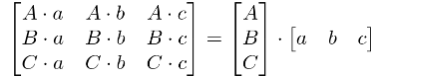
\includegraphics[width=0.5\textwidth]{report_src/separableConv1.png}
            \end{subfigure}
        \end{figure}

        Un kernel est séparable quand sa matrice des poids peut être représentée par le produit de deux vecteurs.
        \\

        Ce calcul est réalisé en faisant deux convolutions unidimensionnelles successives (en X et en Y) sur l'image d'origine en stockant le résultat dans une image intermédiaire.
        La propriété d'associativité de la convolution rend ce calcul possible.

        \[
            x * (N * N)  \iff (x * N) * N
        \]

        La limite de cette méthode c'est que l'on doit passer par une image partielle pour la réalisation du calcul en
        utilisant plus de mémoire que pour une convolution classique.
        \\



    \subsubsection*{Convolution détection de contours} \label{conv_edges}

        Cette méthode prend en paramètre deux kernels de même taille et réalise deux convolutions avec chaque kernel et ensuite calcule le produit des deux.
        Vu que ces deux convolutions sont indépendantes l'une de l'autre on peut se permettre de les réaliser au même temps dans le script et de faire l'addition
        des valeurs absolues résultantes des deux accumulateurs. Comme son nom l'indique cette méthode est utilisée notamment pour faire des convolutions pour la détection de contours
        avec des opérateurs comme Sobel, Kirsch, Prewitt, etc.
    \\
        

    \subsubsection*{Padding} \label{padding}

        Pour éviter l'effet conséquent de la convolution qui est la perte de bords, on applique un padding par extension depuis renderscript.
        \begin{figure}[!h]
            \centering
            \begin{subfigure}[b]{0.3\textwidth}
                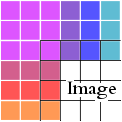
\includegraphics[width=1\textwidth]{report_src/effects/padding.png}
            \end{subfigure}
            \caption*{Exemple de padding par extension.}
        \end{figure} 


    \subsubsection*{Les kernels} \label{kernels}

        Tous les kernels sont définis dans la classe fr.ubordeaux.pimp.util.Kernels. Les kernels de détection de contour (Sobel, Kirsch, Laplace, Prewitt) sont définis
        en variable statique et finale, car leur taille est fixe, les autres sont générés par une méthode. Si on prend le cas du kernel de Gauss, la méthode gauss permet 
        de générer la version séparée du kernel, c'est-à-dire une seule ligne. Les méthodes génératrices de kernel prennent en argument la taille de celui-ci, ce qui sert
        aux effets paramétrables tels que blur et sharpen.

    \subsubsection{Flou gaussien et moyenneur (Blur) : } \label{blur}

        \begin{figure}[!h]
            \centering
            \begin{subfigure}[b]{0.3\textwidth}
                \includegraphics[width=1\textwidth]{report_src/effects/original.jpeg}
            \end{subfigure}
            \begin{subfigure}[b]{0.3\textwidth}
                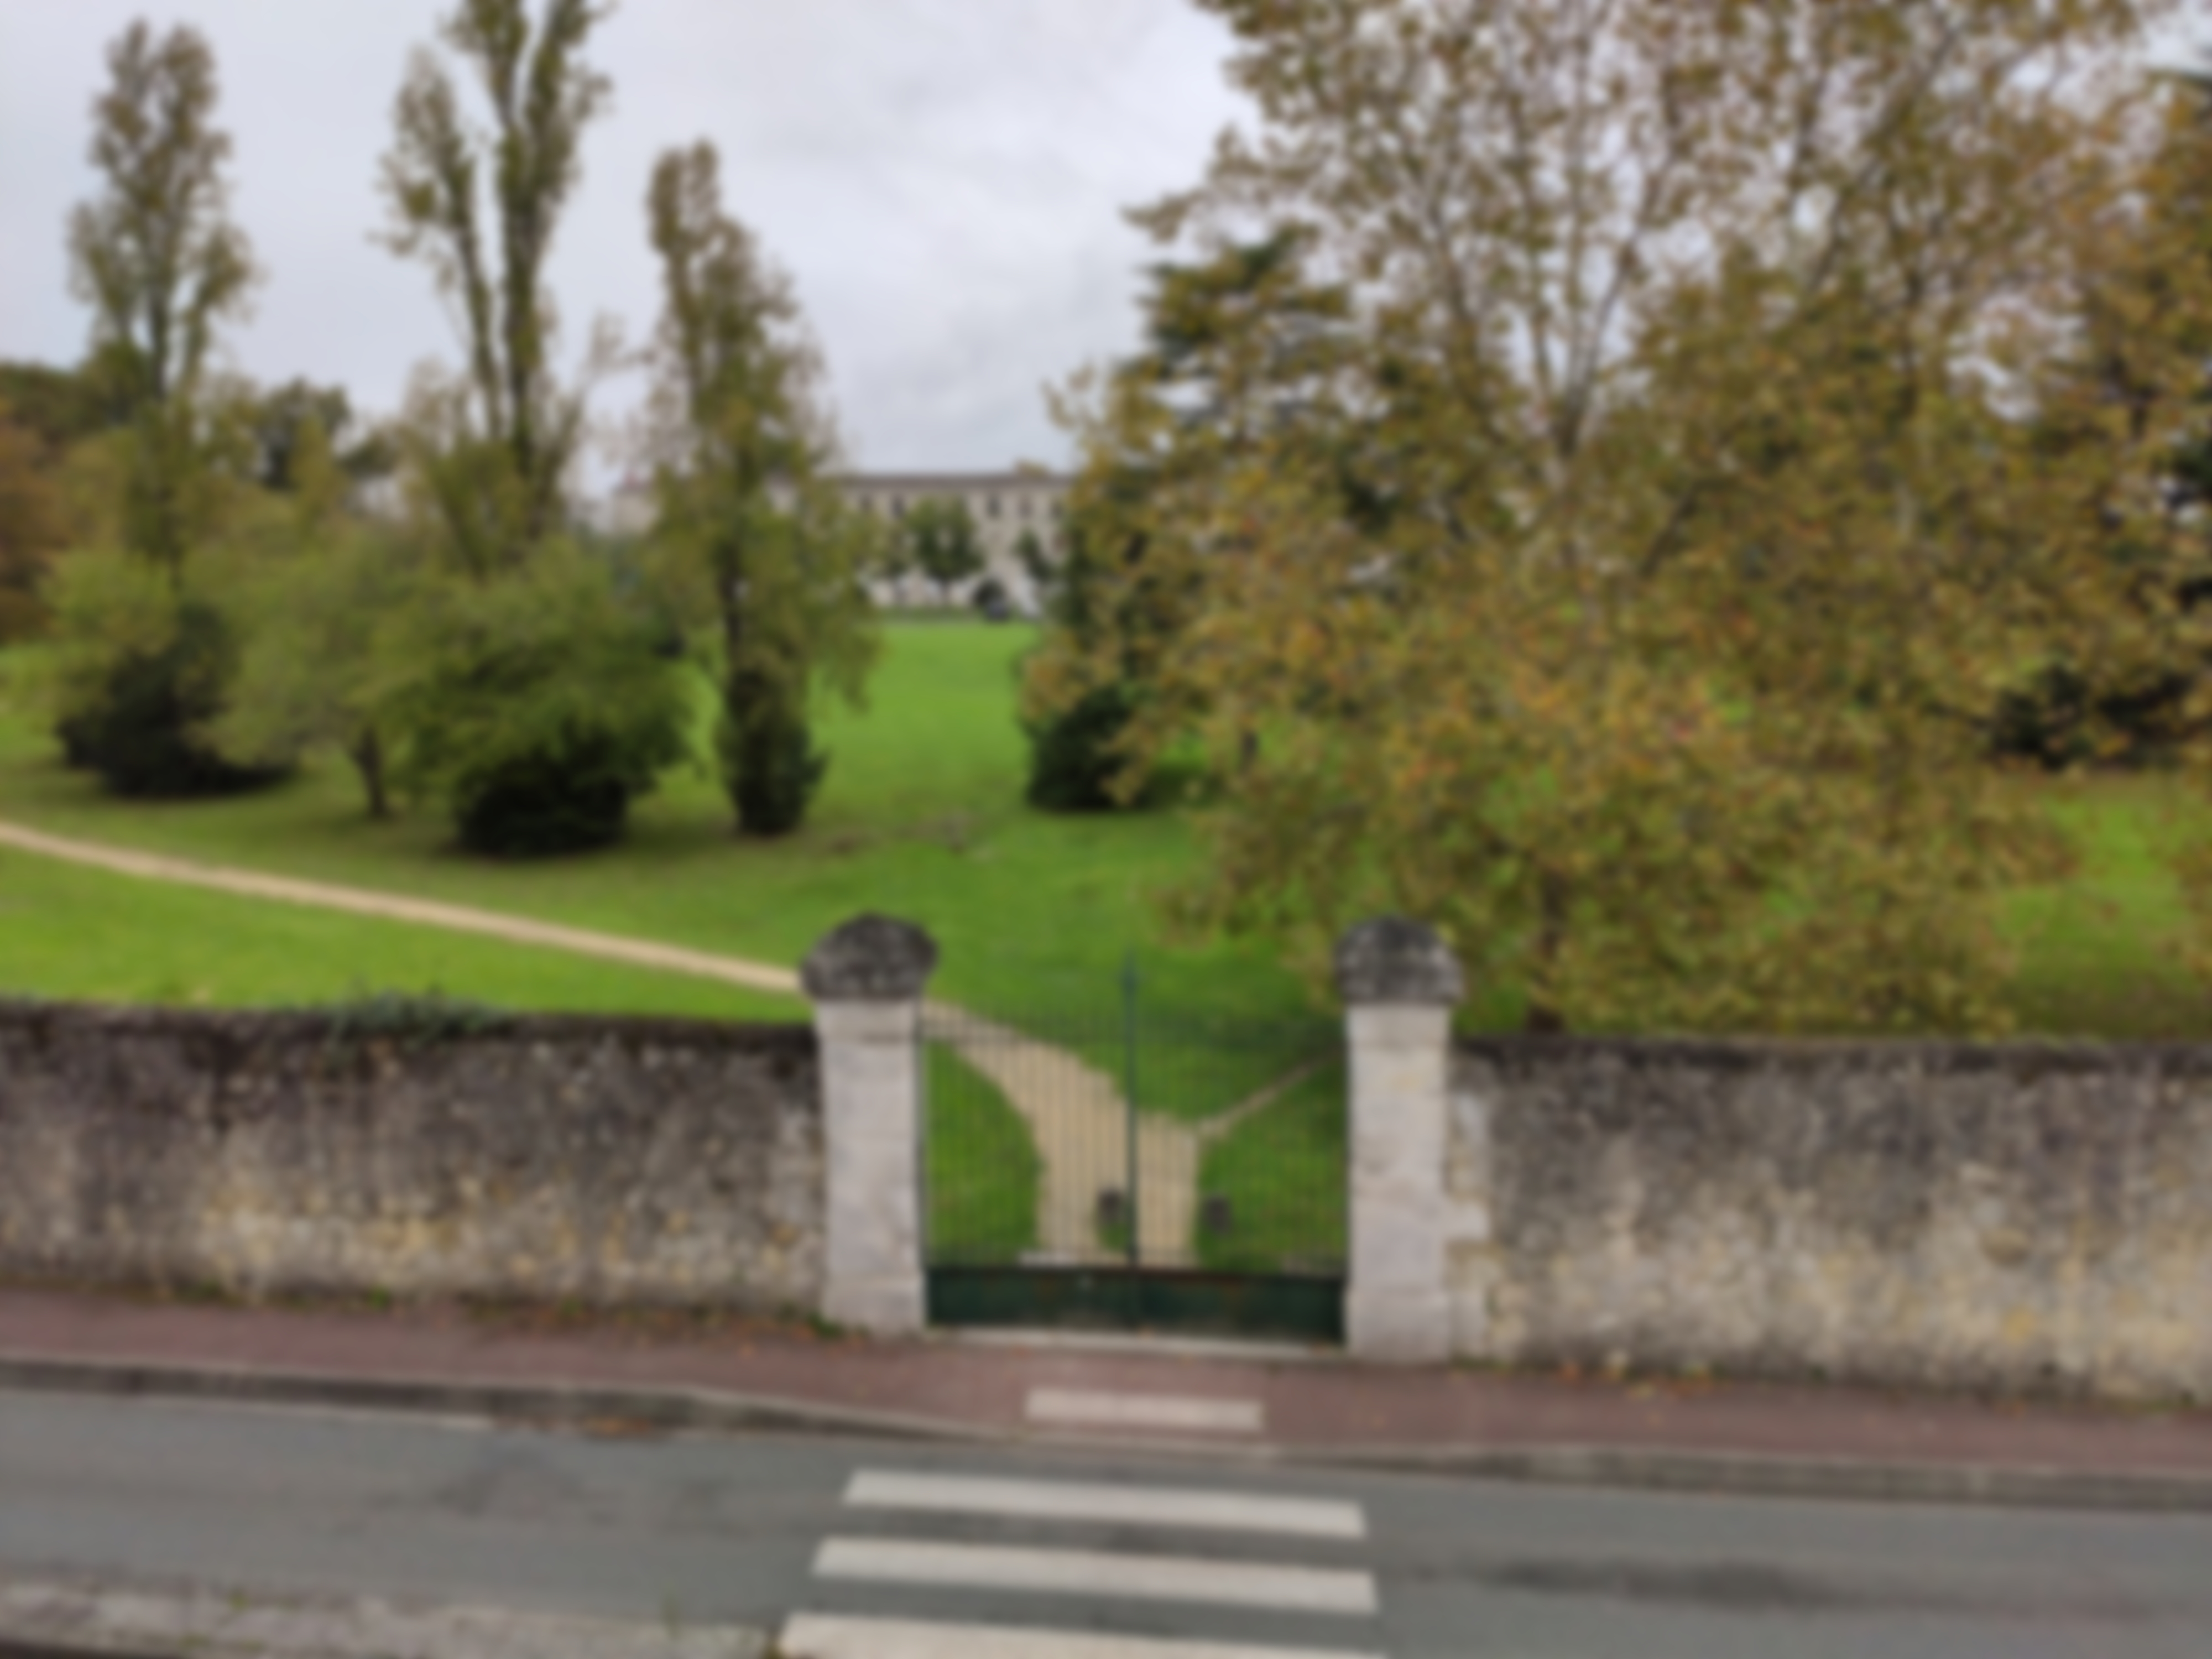
\includegraphics[width=1\textwidth]{report_src/effects/blur.jpeg}
            \end{subfigure}
            \begin{subfigure}[b]{0.3\textwidth}
                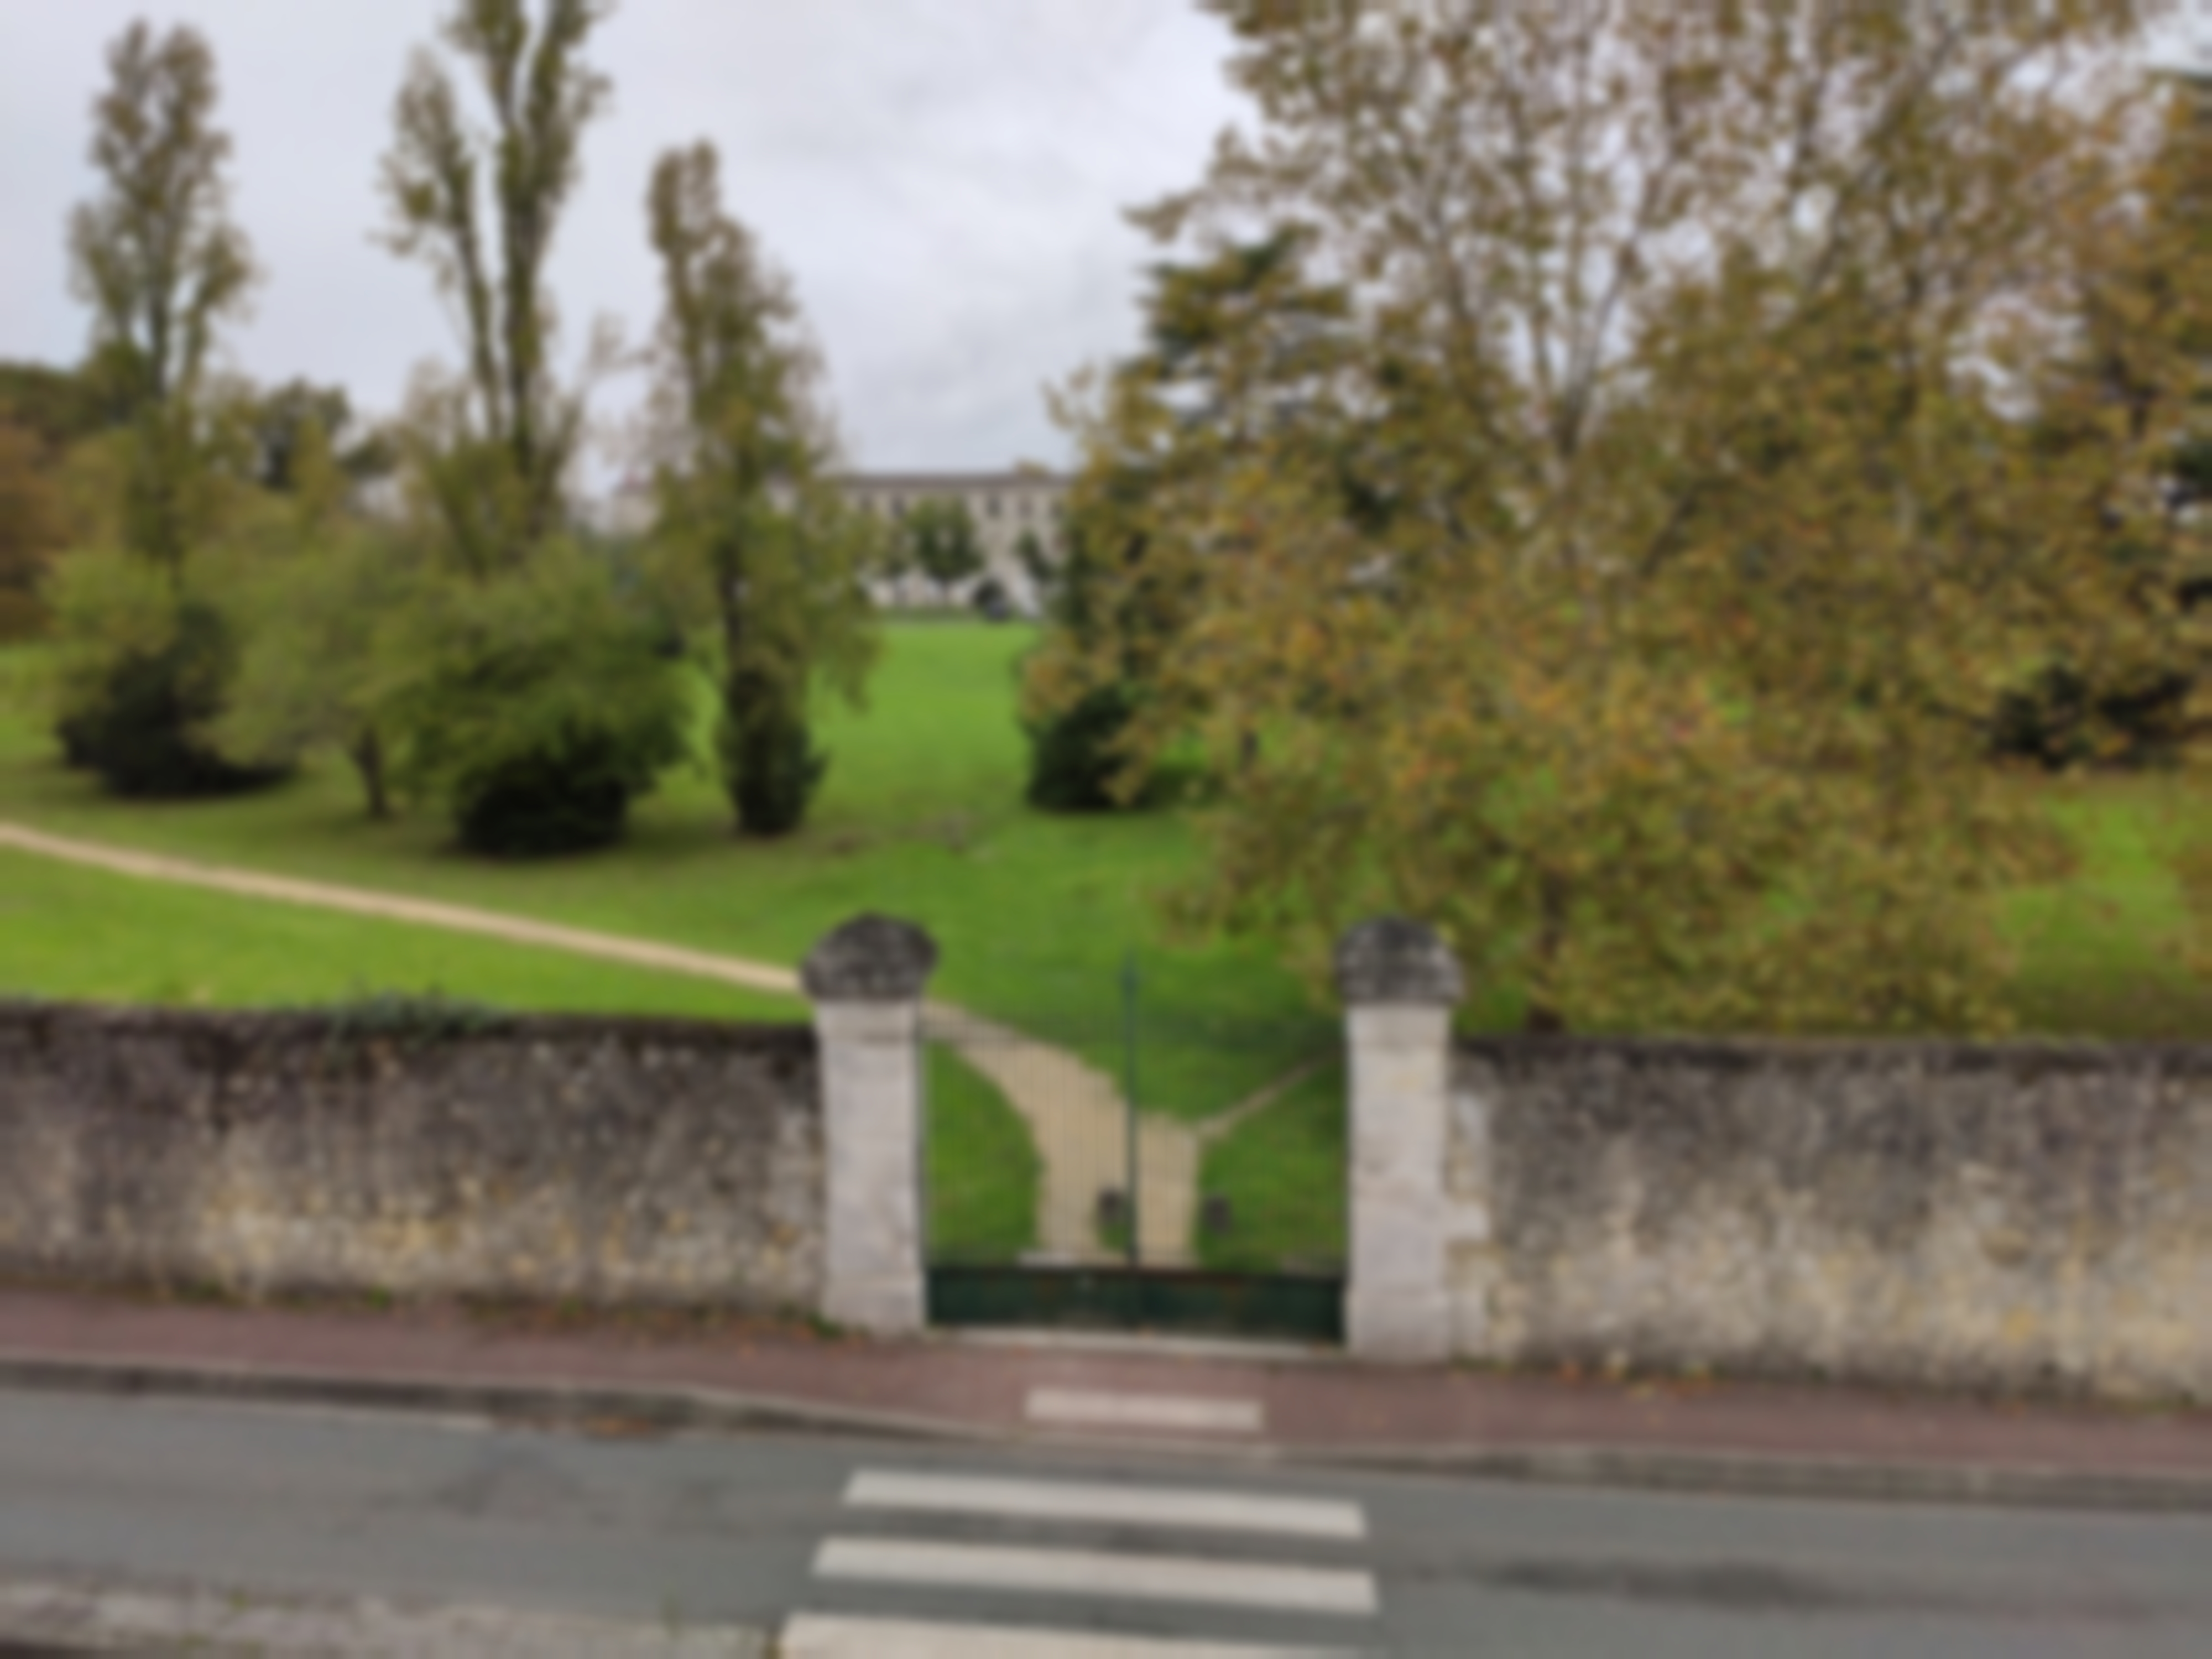
\includegraphics[width=1\textwidth]{report_src/effects/mean.jpeg}
            \end{subfigure}
            \caption*{Comparaison des deux filtres Gaussien(2ème image) et Moyenneur(3ème image) sur une image de taille 4000x3000px.}
        \end{figure} 
        \emph{Méthodes appelantes : Convolution.gaussianBlur(), Convolution.meanBlur()}

        \emph{Scripts : convolution.rs} 
        \\

        Dans la section blur, on réalise des convolutions avec un filtre gaussien ou moyenneur selon le choix de l'utilisateur,
        ces filtres sont réalisés avec une méthode de convolution séparable voir \ref{conv_separable}. Ces kernels sont générés en fonction du progrès de la seekbar qui
        définit une taille de vecteurs sur l'intervalle [3;25]. Pour le filtre gaussien l'écart type noté $\sigma$ est généré en fonction de la taille du kernel en suivant
        cette relation.
        \[
            \sigma  =  \frac{taille_{kernel}}{2}            
        \]

        Cette relation a été définie arbitrairement car il y n'y a pas moyen de calculer avec certitude l'écart type de la fonction gaussienne et en fonction des résultats
        obtenus après une série des tests, nous avons décidé de laisser la relation ci-dessus.

        Pour le filtre moyenneur tout comme le filtre gaussien on génère un vecteur de taille dans l'intervalle [3 - 25] et on les applique verticalement et ensuite horizontalement
        avec la méthode de convolution séparable.
        \\
        
        Cet effet s'applique en temps réel sur l'image et pourtant doit être assez rapide pour son utilisation, il restent encore quelques optimisations à faire
        pour améliorer la fluidité de ce dernier. Voir \ref{limits_conv}.
        \\
        


    \subsubsection{Amélioration de la netteté / Masque flou (Sharpen) : } \label{sharpen}

        \begin{figure}[!h]
            \centering
            \begin{subfigure}[b]{0.4\textwidth}
                \includegraphics[width=1\textwidth]{report_src/effects/original.jpeg}
            \end{subfigure}
            \begin{subfigure}[b]{0.4\textwidth}
                \includegraphics[width=1\textwidth]{report_src/effects/sharpen.jpeg}
            \end{subfigure}
            \caption*{Application de filtre LoG, kernel de taille 13x13, $\sigma$ = 2.6 et image de 4000x3000px}
        \end{figure} 
        
        \begin{figure}[!h]
            \centering
            \begin{subfigure}[b]{0.4\textwidth}
                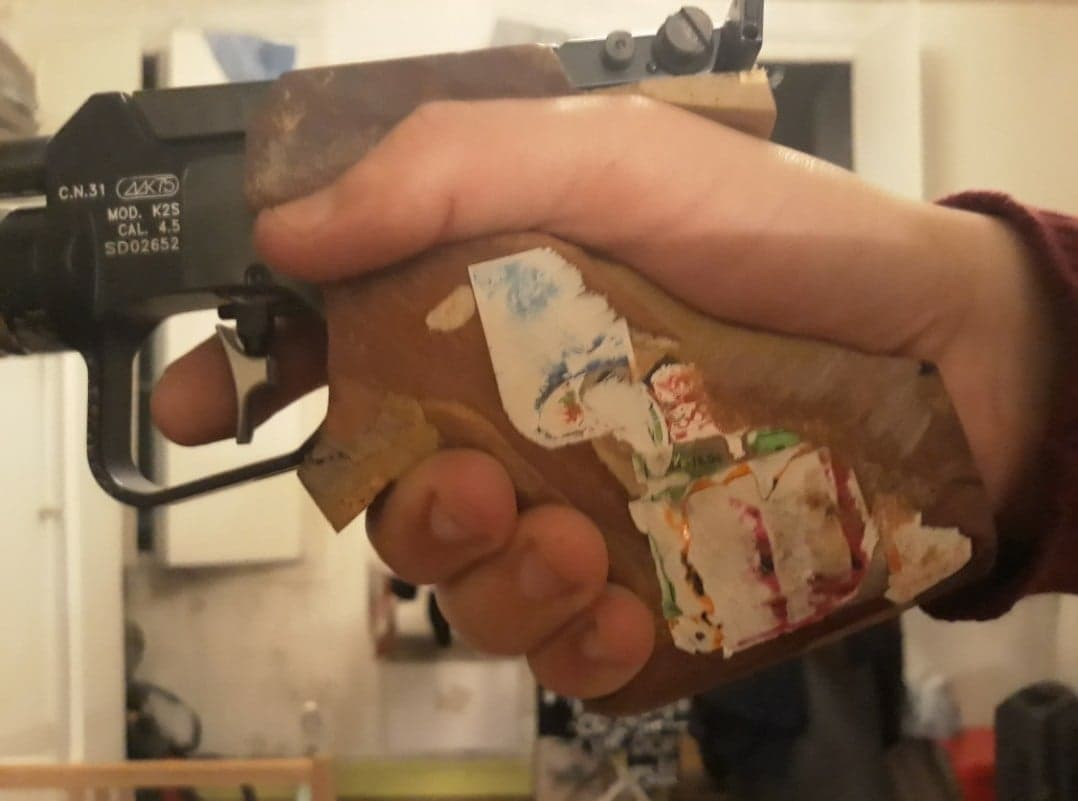
\includegraphics[width=1\textwidth]{report_src/effects/sharpen2.jpg}
            \end{subfigure}
            \begin{subfigure}[b]{0.4\textwidth}
                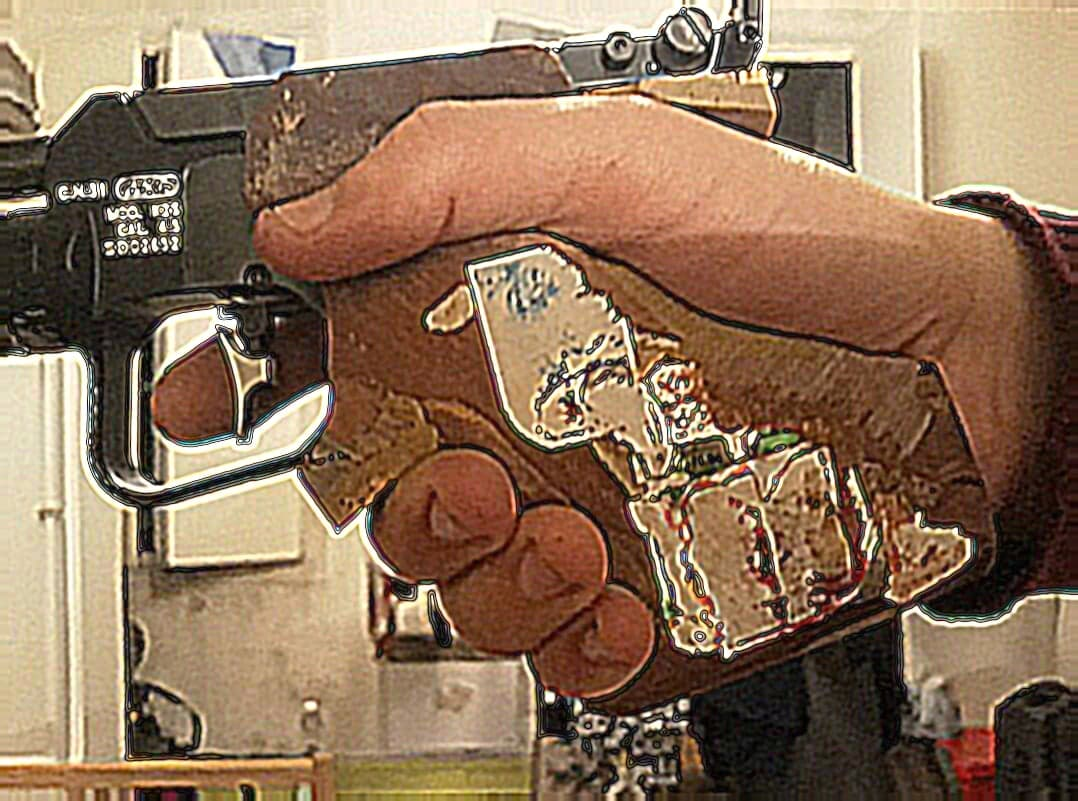
\includegraphics[width=1\textwidth]{report_src/effects/org2.jpg}
            \end{subfigure}
            \caption*{Application de filtre LoG, kernel de taille 9x9, $\sigma$ = 1.8 et image de 1024x724px}
        \end{figure} 
 


        \emph{Méthode appelante : Convolution.sharpen()}

        \emph{Scripts : convolution.rs} 
        \\

        Cet effet consiste à rehausser les contours dans une image également que d'enlever le possible flou dans une image, avec une seekbar en progression.
        Le filtre est réalisé par la convolution d'un filtre suivant une distribution discrète de la fonction "Laplace of Gaussian" (LoG) voir \ref{LoG},
        ce filtre est pourtant séparable en 4 convolutions mais pour histoire d'implémentation et de temps on s'est contenté de garder la version avec la convolution classique.
        Ce filtre est réalisé en temps réel avec des kernels de taille en allant de taille 3x3 jusqu'à 13x13.

        
        \begin{figure}[!h]
            \centering
            \begin{subfigure}[b]{0.8\textwidth}
                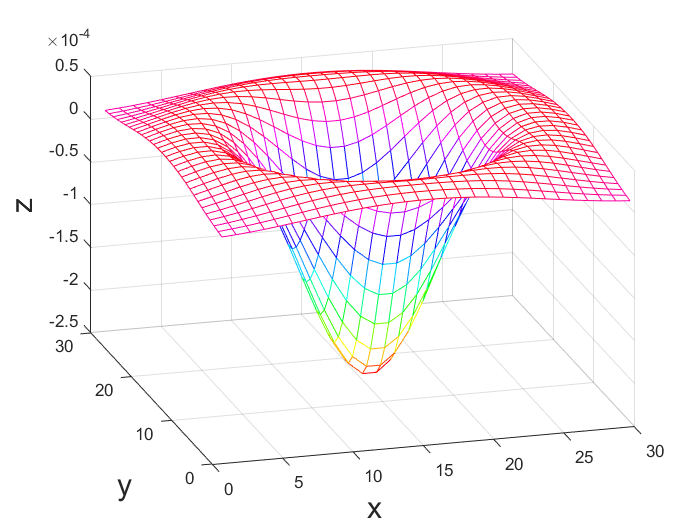
\includegraphics[width=1\textwidth]{report_src/effects/laplacianGaussian.png}
            \end{subfigure}
            \caption*{Représentation graphique de LoG}
        \end{figure}

        Le filtre Laplacien étant très sensible au bruit, c'est pour ceci que généralement on applique une convolution avec un filtre gaussien avant pour supprimer ce bruit,
        cependant avec LoG on peut appliquer une distribution Gaussienne au filtre Laplacien afin d'éviter de faire 2 convolutions.
        \\
        Par ailleurs pour reproduire cet effet de rehaussement de contours on peut
        flouter l'image originale avec un filtre gaussien (suppression du bruit), ensuite calculer la charte de contours avec un filtre laplacien et puis combiner l'image d'origine avec le résultat
        de la charte de contours.
        Grâce à cette fonction on peut compresser cette procédure à une génération de kernel suivi d'une seule convolution de ce dernier.
        \\

        Comme pour les filtres précédents l'écart type du LoG est définit comme suit :
        \[            
            \sigma =  \frac{taille_{kernel}}{5}
        \]

        Comme pour l'écart type gaussien ce sigma a été choisi en fonction des résultats.
        \newpage

    \subsubsection{Détection des contours (Néon) : } \label{neon}

        \begin{figure}[!h]
            \centering
            \begin{subfigure}[b]{0.4\textwidth}
                \includegraphics[width=1\textwidth]{report_src/effects/original.jpeg}
            \end{subfigure}
            \begin{subfigure}[b]{0.4\textwidth}
                \includegraphics[width=1\textwidth]{report_src/effects/sobel.jpeg}
            \end{subfigure}
            \caption*{Opérateur de Sobel sur une image de taille 4000x3000px}
        \end{figure} 
        
        \begin{figure}[!h]
            \centering
            \begin{subfigure}[b]{0.4\textwidth}
                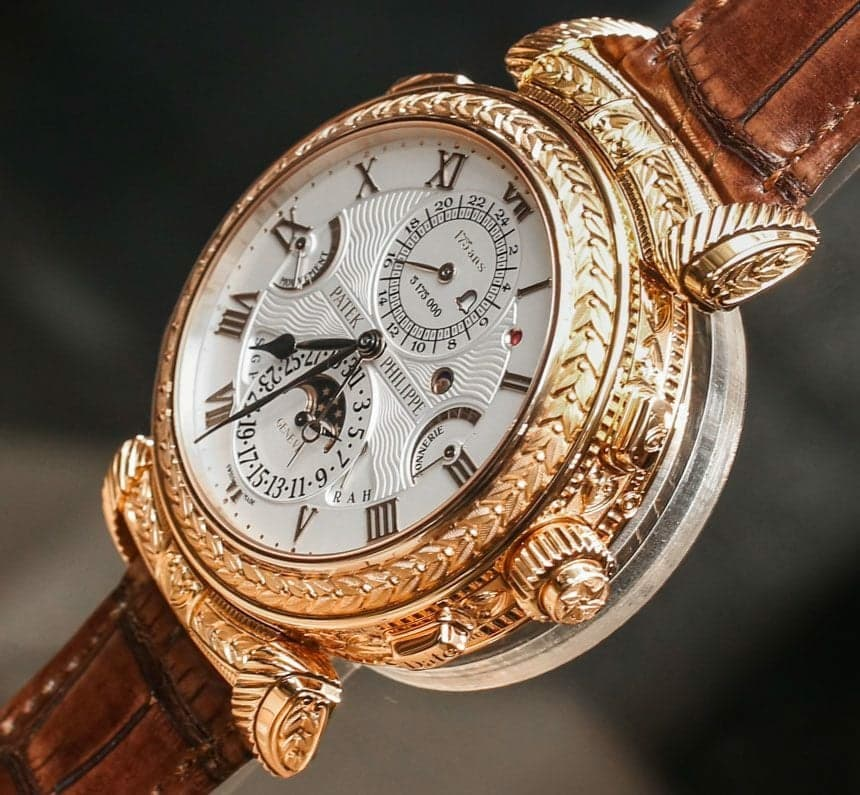
\includegraphics[width=1\textwidth]{report_src/effects/org3.jpg}
            \end{subfigure}
            \begin{subfigure}[b]{0.4\textwidth}
                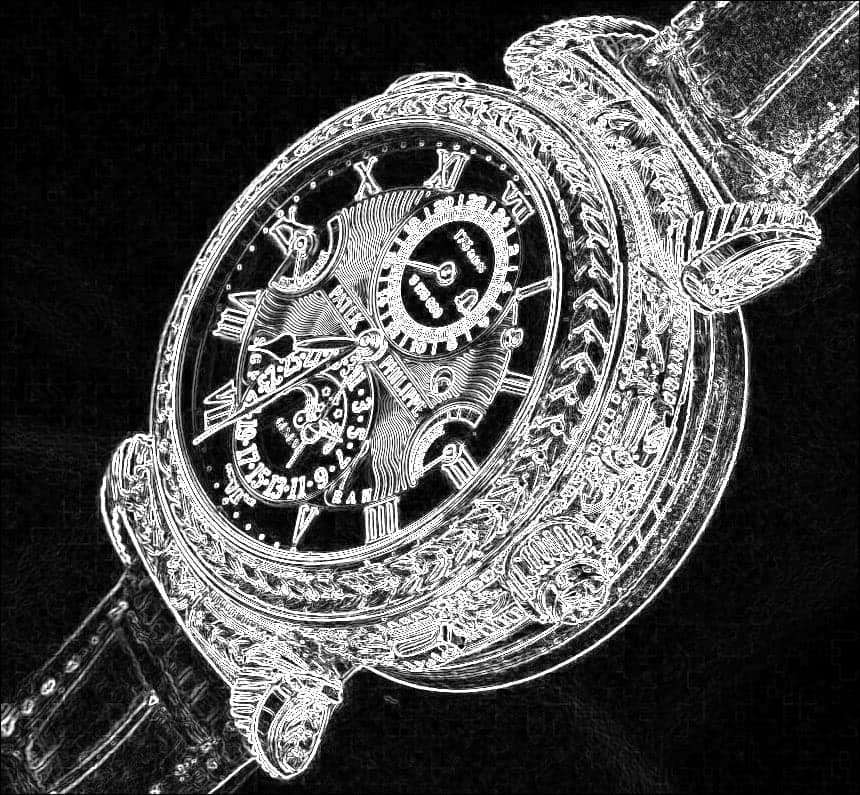
\includegraphics[width=1\textwidth]{report_src/effects/sobel3.jpg}
            \end{subfigure}
            \caption*{Opérateur de Sobel sur une image (passée en échelle de gris) de taille 860x795}
        \end{figure} 

        \emph{Méthode appelante : Convolution.neonSobel()}

        \emph{Scripts : convolution.rs} 
        \\

        Cet effet consiste à créer un effet "Neon" sur une image en utilisant des opérateurs de détection de contours (voir \ref{edge_source}) comme Sobel, Prewitt et aussi d'un filtre Laplacien qui est également détecteur de contours.
        Nous avons mis 3 boutons de type \textbf{RadioButton} pour sélectionner le type de kernel à utiliser et ainsi voir les différences de chacun sur l'image.
        \\
        
        Les valeurs résultantes de la convolution en "Neon" ne sont pas normalisées par extension linéaire, elles sont justes tronquées entre [0 - 255] à cause de ce troncage on risque de perdre des données sur l'image,
         surtout avec des images avec beaucoup des contours, pour avoir donc un résultat plus fidèle, faudrait passer par une image intermédiaire, calculer 
        leurs respectifs minimum et maximum pour ensuite normaliser l'image précédente cette solution est discutable puisque on devrait réallouer une image de plus en mémoire et rajouter quelques parcours en plus sur l'image. Cependant
        nous avons essayé de \textbf{calculer la valeur maximale théorique} pour normaliser mais ceci donne des résultats très sombres par rapport à l'image originale, nous avons décidé donc de garder l'ancienne normalisation et considérer le fait de normaliser par extension linéaire.
        \\

    \subsubsection{Remarques et limites} \label{limits_conv}

        
        \begin{itemize}
            \item {Un des points de réflexion sur la convolution c'est que jusqu'à présent elle est réalisée sur les 3 canaux RGB, ce qui est assez lourd au niveau de calcul,
            cependant on pourrait passer l'image en échelle de gris et la faire seulement sur un des canaux ou passer pour l'espace HSV en utilisant la value ou la saturation.}
            \item {Tous les calculs de convolution sont uniquement réalisées avec des nombres "flottants", ceci est un choix d'implémentation car renderscript, possède plus de support
            pour réaliser des opérations flottantes que pour des opérations sur des entiers qui en plus sont codés en 8 bits dans une image. Pour éviter donc les erreurs de débordement et pour garder une bonne qualité de l'image
            on a décidé de travailler exclusivement avec des flottants, même si ceci peut être pénalisant au niveau de performance, cependant des tests sont à prévoir pour le prochain rendu pour essayer
            d'améliorer la performance sur des filtres comme "Blur"\ref{blur} et "Sharpen"\ref{sharpen}.}
            \item {Pour la convolution classique et séparable les valeurs sont normalisées en prennant le résultat d'opération de voisinage pour un pixel donné
            divisé par la somme des poids des éléments du kernel. Ceci marche assez bien sauf pour les kernels avec des valeurs négatives notamment ceux de détection de contours comme Laplace, Sobel, Prewitt, etc (Voir \ref{conv_edges}).
            }

            \item {Il y a quelques améliorations de performances à faire pour les convolutions réalisées en temps réel comme pour les effets Blur et Sharpen, une optimisation par échantillonnage linéaire\ref{linear_sampling}
            est à tester ainsi que le calcul par des entiers au lieu de flottants.}

            \item {Une des plus grandes limites des effets de convolution c'est que dû à notre implémentation de sauvegarde\ref{file_effets}, on ne peut malheureusement pas garantir le même résultat sur l'image sauvegardée que sur l'aperçu.
            Vu que la réponse des filtres de convolution sur une image précise sont fortement liés à la taille de l’image et que l'image d'aperçu est en général plus petite que l'originale, de fois on peut se retrouver avec une image sauvegardée avec un flou moins fort ou avec une détection de bords plus faible que sur l'aperçu
            ainsi qu'une sensibilité plus forte au bruit.\ref{remarques_code}}
        \end{itemize} 

\newpage

\subsection{CLAHE}

\begin{figure}[!h]
    \centering
    \begin{subfigure}[b]{0.4\textwidth}
        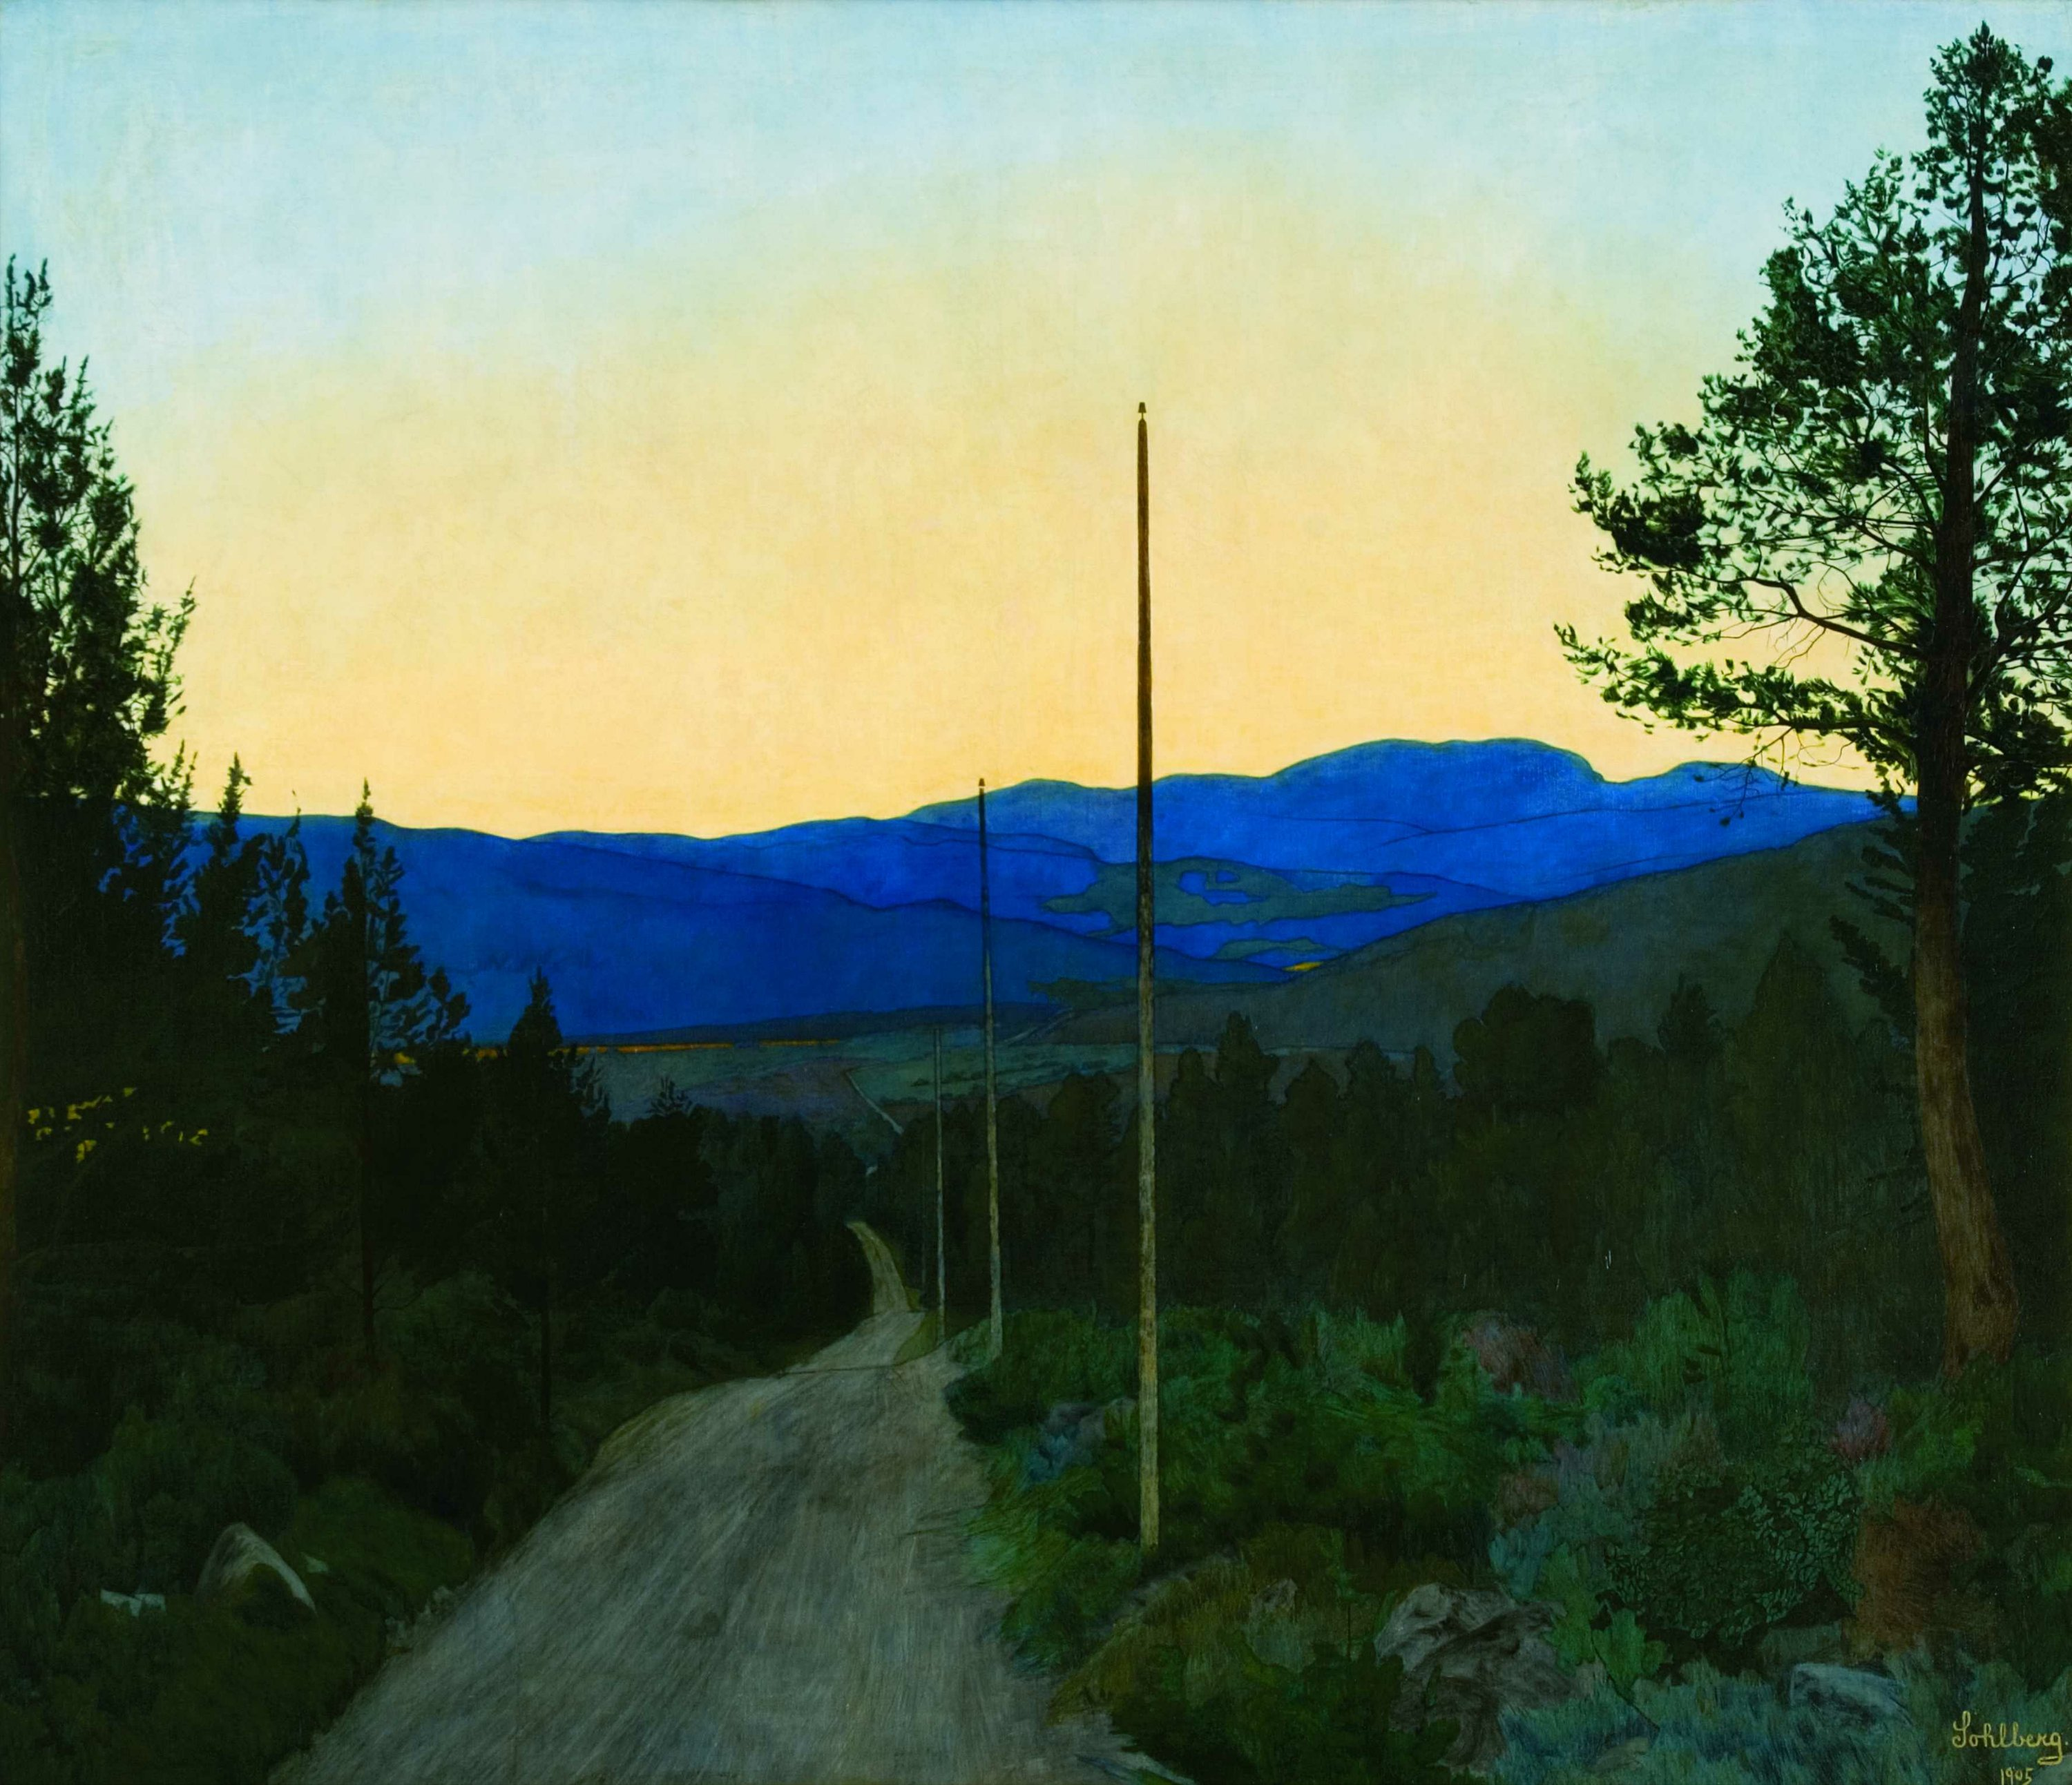
\includegraphics[width=1\textwidth]{report_src/effects/CLAHE_before.jpg}
    \end{subfigure}
    \begin{subfigure}[b]{0.4\textwidth}
        \includegraphics[width=1\textwidth]{report_src/effects/CLAHE_after.jpeg}
    \end{subfigure}
    \caption*{CLAHE 8x8 avec clip = 4.0}
\end{figure} 


\emph{Méthode appelante : CLAHE.CLAHE()}

\emph{Scripts : cumulativeHistogram.rs, assignCLAHELuts.rs} 
\\

CLAHE est une variation de l'algorithme d'égalisation d'histogramme adaptative (AHE) qui performe 
une égalisation sur différentes cases de l'image. Le fait de diviser l'image en cases et de traiter celles-ci 
de manière indépendante permet d'accentuer le contraste de chacune d'elle de manière locale, mettant ainsi en valeur l'entièreté de l'image.
CLAHE, en plus d'AHE, implémente une limitation de contraste (d'où "CL" pour Contrast-Limited) qui permet d'éviter une accentuation 
trop importante pour des zones où cela n'est pas nécessaire (exemple : ciel, plafond ou quoique ce soit de relativement uniforme).
Pour éviter les artefacts entre chaque case, nous avons choisi la méthode de l'interpolation bilinéaire. Voici un schéma explicatif :
\\

\begin{figure}[!h]
    \centering
    \begin{subfigure}[b]{0.8\textwidth}
        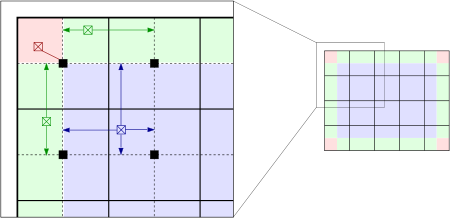
\includegraphics[width=1\textwidth]{report_src/CLAHE.png}
    \end{subfigure}
\end{figure} 

La grille représente le découpage de l'image en cases. Il existe une LUT extraite de l'histogramme cumulé pour chaque case,
seulement cette LUT est valable uniquement pour le centre de la case (en noir sur le schéma ci-dessus). 
En rouge (dans les coins), on n'effectue pas d'intrepolation, la valeur du pixel est directement celle de la LUT. En vert, 
on applique une interpolation linéaire, et en bleu une interpolation bilinéaire. Dans chaque cas, on interpole entre les valeurs
données par les LUT voisines pour la valeur du pixel courant.
\\

Notre implémentation offre deux paramètres que l'utilisateur modifie à l'aide de seekbars :
\begin{itemize}
    \item{dimension de la grille de découpage, allant de 3x3 à 8x8 (8x8 étant le maximum recommandé)}
    \item{clip limit : waiting for Ricardo..}
\end{itemize}

\subsubsection{Remarques et améliorations}

Notre algorithme calcule et assigne les LUTs de chaque région de manière séquentielle. Il est en théorie possible d'appliquer CLAHE en parallèle
sur chaque région, seulement RenderScript rend la tâche difficile. En effet, le calcul d'histogramme cumulé s'effectue par un "reduction kernel" et il n'est 
pas possible de lancer en parallèle de tels scripts. Nous avons donc choisi d'implémenter deux boucles parcourant toutes les cases,
la première calculant la LUT résultante de l'histogramme cumulé et la deuxième assignant ces LUTs aux pixels par le biais de l'interpolation bilinéaire.
\\

Nous avons conscience que la présence de CLAHE dans notre application n'est pas forcément vendeur pour le grand public 
et que l'utilisateur moyen ne recherche pas spécialement cet "effet", cependant nous avons choisi de l'implémenter pour sa popularité dans le domaine
de l'imagerie médicale, de la photographie sous-marine, et également car son implémentation constituait un challenge technique intéressant.
\clearpage

%%%%%%%%%%%%%%%%%%%%%%%%%%%%%%%%%%%%%%%%%%%%%%%%%%%%%
%Structure du projet:
%%%%%%%%%%%%%%%%%%%%%%%%%%%%%%%%%%%%%%%%%%%%%%%%%%%%%
\section{Structure du projet :}

\subsection{Structure graphique Android et navigation :}\label{navig}
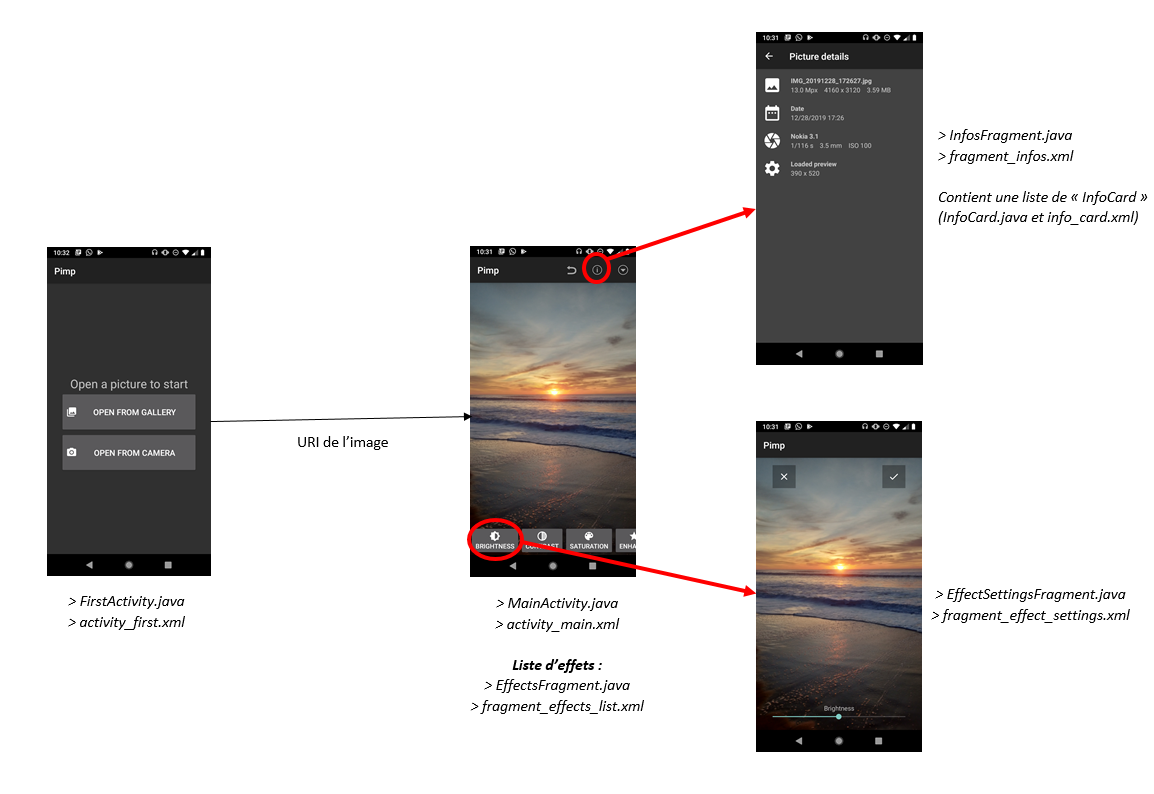
\includegraphics[width=1\textwidth]{report_src/app_flowchart_fragments.PNG}

Pour afficher certains éléments d'interface comme par exemple les informations de l'image (bouton \faInfoCircle) nous utilisons des \textbf{Fragment}. En effet une activité supplémentaire n'est pas nécessaire car cette petite partie de l'application ne correspond pas à un point d'entrée de l'application. Par ailleurs changer de fragment (plutôt que de changer directement de layout) pourrait faciliter l'implémentation d'une interface différente, pour tablette par exemple.
De même, la liste d'effets et leurs paramètres respectifs sont aussi contenus dans des fragments séparés. Cela permet de gérer plus simplement leur affichage et de clarifier le code.
\\

On notera que dans la structure actuelle de l'application, l'image actuellement éditée est contenue et manipulée depuis l'activité principale. Les fragments n'apportent à l'application que des éléments d'interface.
\\

Une seconde activité est cependant utilisée pour la page d'accueil à l'ouverture de l'application, cette \textbf{FirstActivity} utilise des méthodes génériques de \textbf{ActivityIO} afin de gérer l'ouverture de la galerie ou de la caméra. L'application reste dans cette activité tant qu'une \textbf{Uri} valable ($\approx$ chemin) n'a pas été sélectionnée. Ensuite cette Uri est transférée à \textbf{MainActivity} qui va alors charger cette première Image, en cas de problème de chargement l'application peut retourner dans FirstActivity.

\subsection{Classe \textbf{Image} :} \label{classeImage}
Cette classe a été conçu comme une alternative à l'utilisation directe de la classe \textbf{Bitmap} fournie par Android.
\\
Le coeur de la classe est évidement une instance de Bitmap, qu'il est possible de récupérer à tout moment. Par ailleurs la classe offre des fonctionnalités supplémentaires, parmi celle ci notamment la possibilité de restaurer l'image à son état au moment de sa création ou de son chargement via la méthode \textbf{reset()}, ou d'annuler les dernières modifications apportées par un effet grâce aux méthodes \textbf{quicksave()} et \textbf{discard()}.
\\

On notera la nécessité pour Image d'avoir la référence d'une Activité de l'application, en effet elle est requise à plusieurs moments par les librairies Android pour charger la Bitmap en mémoire.

\subsubsection{Classe \textbf{ImageInfo} :}
La classe Image \ref{classeImage} génère et garde une instance de la classe \textbf{ImageInfo}, cette classe contient un grand nombre de valeurs à propos de l'Image (dimensions, coordonnées GPS, date de prise de vue, ...).
\\
L'idée de cette classe était d'empaqueter toutes ces informations afin de faciliter le passage de ces informations à travers des Fragments ou des Activités (voir \ref{navig}). On notera que tous les accesseurs appliquent des opérations de formatage sur ces données, certaines opérations pourraient être déplacées dans les constructeurs si elles venaient à être utilisées régulièrement.


\subsubsection{File d'effets :} \label{file_effets}
Pour pouvoir exporter l'image éditée, il est nécessaire de ré appliquer sur l'image d'origine tout les effets appliqués à l'image affichée dans l'application.
\\
C'est pourquoi la classe Image permet d'empaqueter une Queue de \textbf{BitmapRunnable}. Les BitmapRunnable permettent de transporter des méthodes d'effets, en effet en définissant la méthode \textbf{run()} à l'instanciation de ces objets on peut empaqueter un effet applicable à un objet \textbf{Bitmap}. Ce qui permet de passer n'importe quel effet venant de n'importe quel auteur, ce qui renforce la modularité des effets et de la classe Image.
\\
Dans la version actuelle cette Queue d'effets n'est qu'une liste "bloc-note" que l'utilisateur de Image peut utiliser, dans cette application les effets appliqués sont notés au fur et à mesure et cette liste est ensuite récupérée à l'export de l'image.


\subsection{AsyncTasks}
Les 3 classes du package \textbf{fr.ubordeaux.pimp.task} héritent de la classe Android \textbf{AsyncTask} et permettent d'exécuter certaines opérations en arrière plan, donc sans bloquer l'interface utilisateur.
\\
Ainsi \textbf{LoadImageUriTask} et \textbf{ApplyFilterQueueTask} permettent respectivement de charger une image et de l'exporter, elles s'occupent d'afficher un petit logo de chargement et de lancer les calculs.
\\
\textbf{ApplyEffectTask} est un peu différente, elle permet de mettre en arrière plan le calcul d'application d'un effet. Elle fonctionne pour n'importe quel effet, pour ce faire elle a besoin d'un paramètre, le type d'effet sous la forme d'un \textbf{Runnable}.

\subsection{Packages utilitaires :}
De nombreuses classes du code permettent une factorisation et une clarification du code en offrant des méthodes pratiques, généralement statiques. Parmi ces classes on pourra retrouver:
\\

La classe \textbf{Utils} qui offre des méthodes pour récupérer la taille de l'écran, pour calculer un ratio de redimensionnement, pour manipuler des chemins d'image ou régler des problèmes d'orientation d'image.
\\

La classe \textbf{BitmapIO} permet d'effectuer le chargement d'une Bitmap de plusieurs manières, depuis les resources ou un autre emplacement du téléphone, et avec la taille voulue.
\\

La classe \textbf{ActivityIO} permet de gérer l'ouverture de l'application de galerie ou de caméra et d'en récupérer le retour, le tout en gérant les permissions de l'application.
\\

Enfin la classe \textbf{Kernels} offre des méthodes de génération de noyau de convolution permettant de créer différents effets.

\clearpage

%%%%%%%%%%%%%%%%%%%%%%%%%%%%%%%%%%%%%%%%%%%%%%%%%%%%%
% Tests de performance :
%%%%%%%%%%%%%%%%%%%%%%%%%%%%%%%%%%%%%%%%%%%%%%%%%%%%%
\section{Performances :}
Tous les tests de performance présentés dans cette section ont été effectués sur un Nokia 3.1.
Voici un résumé de ses caractéristiques :
\begin{itemize} [label=\textbullet]
  \item \textbf{Version} : Android 9
  \item \textbf{Résolution}	: 1440 x 720 pixels
  \item \textbf{Cadence processeur} : 1.5 GHz
  \item \textbf{RAM} : 2 Go
\end{itemize}

\subsection{Temps d'exécution :}

Les temps d'exécution présentés ne tiennent pas compte du premier temps de chargement du script renderscript.
\\

Voici les temps d'exécution \textbf{sur 10 appels} de chaque effet pour une image de dimension \textbf{425x265px}.
\\

\begin{tabular}{||l||c|c||c|c||}
    \hline
    \hline
    \textbf{Effet} & \textbf{Temps d'exécution en ms} (min | max | moyenne | écart-type)\\
    \hline
    \hline
    Brightness & 12.0 | 46.0 | 16.9 | 9.73\\
    \hline
    Contrast & 16.0 | 28.0 | 20.5 | 3.80\\
    \hline
    Saturation & 13.0 | 23.0 | 15.2 | 2.929\\
    \hline
    Enhance & 22.0 | 32.0 | 26.4 | 3.00\\
    \hline
    To gray & 9.0 | 11.0 | 10.0 | 0.63\\
    \hline
    Invert & 8.0 | 10.0 | 8.4 | 0.66\\
    \hline
    Change hue & 11.0 | 18.0 | 13.4 | 1.90\\
    \hline
    Keep hue & 10.0 | 11.0 | 10.6 | 0.48\\
    \hline
    Gaussian blur 3x3 & 17.0 | 21.0 | 18.8 | 1.24\\
    \hline
    Gaussian blur 25x25 & 47.0 | 51.0 | 48.5 | 1.36\\
    \hline
    Mean blur 3x3 & 16.0 | 19.0 | 18.2 | 1.07\\
    \hline
    Mean blur 25x25 & 54.0 | 60.0 | 55.8 | 1.72\\
    \hline
    Sharpen 3x3 & 21.0 | 25.0 | 23.6 | 1.11\\
    \hline
    Sharpen 13x13 & 136.0 | 165.0 | 146.3 | 8.97\\
    \hline
    Sobel filter & 21.0 | 31.0 | 24.7 | 2.53\\
    \hline
    Prewitt filter & 24.0 | 27.0 | 25.3 | 1.09\\
    \hline
    Laplacian filter & 22.0 | 26.0 | 23.6 | 1.11\\
    \hline
    \hline
  \end{tabular}
\\
\newpage
Voici les temps d'exécution \textbf{sur 10 appels} de chaque effet pour une image de dimension \textbf{3400x2118px}.
\\

\begin{tabular}{||l||c|c||c|c||}
    \hline
    \hline
    \textbf{Effet} & \textbf{Temps d'exécution en ms} (min | max | moyenne | écart-type)\\
    \hline
    \hline
    Brightness & 105.0 | 311.0 | 145.8 | 56.95\\
    \hline
    Contrast & 163.0 | 202.0 | 176.9 | 12.73\\
    \hline
    Saturation & 209.0 | 236.0 | 221.4 | 8.34\\
    \hline
    Enhance & 256.0 | 268.0 | 261.3 | 3.74\\
    \hline
    To gray & 125.0 | 138.0 | 129.6 | 3.35\\
    \hline
    Invert & 84.0 | 105.0 | 94.7 | 8.69\\
    \hline
    Change hue & 218.0 | 319.0 | 231.7 | 29.48\\
    \hline
    Keep hue & 162.0 | 181.0 | 168.4 | 5.06\\
    \hline
    Gaussian blur 3x3 & 245.0 | 265.0 | 256.4 | 6.63\\
    \hline
    Gaussian blur 25x25 & 1453.0 | 1484.0 | 1462.2 | 9.08\\
    \hline
    Mean blur 3x3 & 245.0 | 652.0 | 358.5 | 146.25\\
    \hline
    Mean blur 25x25 & 1461.0 | 2447.0 | 1716.6 | 318.34\\
    \hline
    Sharpen 3x3 & 433.0 | 524.0 | 471.7 | 25.25\\
    \hline
    Sharpen 13x13 & 5112.0 | 8974.0 | 5679.2 | 1119.49\\
    \hline
    Sobel filter & 450.0 | 497.0 | 469.4 | 14.47\\
    \hline
    Prewitt filter & 452.0 | 490.0 | 472.5 | 10.39\\
    \hline
    Laplacian filter & 411.0 | 533.0 | 460.4 | 40.08\\
    \hline
    \hline
  \end{tabular}

\subsection{Mémoire :}
TODO montrer l'ancienne instance d'image se faire garbage collecter ? voir remarques

TODO
\clearpage

%%%%%%%%%%%%%%%%%%%%%%%%%%%%%%%%%%%%%%%%%%%%%%%%%%%%%
% Remarques et améliorations :
%%%%%%%%%%%%%%%%%%%%%%%%%%%%%%%%%%%%%%%%%%%%%%%%%%%%%
\section{Remarques et améliorations  :}

\subsection{Remarques sur le code} \label{remarques_code}
A propos de la classe \textbf{Image} \ref{classeImage}, nous sauvegardons systématiquement une copie des pixels d'origine de l'Image, de plus si un appel à \textbf{quickSave()} est effectué une 3ème copie de l'Image est chargée en mémoire. Image offre cependant des constructeurs pour charger une image proportionnée à l'écran de l'appareil. Le risque de débordement mémoire est donc largement évité par cette limitation de taille.
\\

Lors du chargement d'une nouvelle image, nous ré-instancions un objet de la classe Image. Ce qui veut techniquement dire que jusqu'au prochain passage du ramasse miette Android, deux images sont en mémoires, donc deux Bitmap et deux tableaux de pixels (la copie originale des Images, voir \ref{classeImage}). C'est un élément discutable cependant notre application limite la taille des Images chargées. Ce qui évite largement les dépassements mémoire.
\\

Dans la partie \ref{navig} nous créons une \textbf{MainActivity} après avoir récupéré une \textbf{Uri}, il aurait été idéal de rester dans \textbf{FirstActivity} jusqu'à chargement complet de la première image. Ce qui éviterait un éventuel aller-retour entre les activités en cas d'erreur. Cependant les limites de \textbf{Parcelable} \ref{parcelable} ainsi que l'utilisation d'une \textbf{AsyncTask} (donc un Thread différent) nous ont contraint à garder ce fonctionnement.
\\

Par ailleurs notre gestion des fragments n'est finalement pas très optimale, en effet à cause des difficultés du passage de paramètre entre eux (voir section suivante) nous n'avons pas un code très constant puisque parfois nous utilisons des Parcelable ou des Bundle mais parfois nous passons des paramètres aux constructeurs ou aux mutateurs.
\\

Comme dit précédemment nous chargeons une image plus petite que l'originale afin d'optimiser la fluidité de l'application, à l'export en revanche le fichier image d'origine est chargé pour subir la même suite d'effets. Cette méthode ne permet pas d'empêcher un crash mémoire si l'image est immense (image d'appareil photo par exemple). On pourrait à l'avenir complexifier l'export pour charger et sauvegarder par morceaux le fichier image. Cependant ce n'est pas une priorité, la majorité des utilisateurs de l'application vont éditer des images venant d'appareils mobiles qui dépassent rarement les 20Mpx.
Nous avons défini une limite de 5000x5000px comme taille d'image en entrée, les images au dessus de cette taille seront redimensionnées en facteur $x^2$ à la sauvegarde pour assurer la fluidité de l'application.
\\

Le fait de charger l'image d'origine pour refaire les effets a comme conséquence que certains effets, notamment ceux de convolution aient une différence entre l'aperçu et l'image sauvegardée\ref{limits_conv}. Une possible solution à ce problème pourrait être d'afficher ou travailler avec un "crop" de l'image d'origine pour ces effets là.
\\

\subsection{Remarques sur les librairies Android}
Lors de la construction des instances d'\textbf{Image}\ref{classeImage}, nous devons passer la référence de l'activité contextuelle à l'Image, bien que pas très intuitif cette référence est nécessaire car utilisée par les méthodes de \textbf{Bitmap} de chargement d'image.
\\

\label{parcelable}
Pour manipuler des objets d'une activité à l'autre ou entre fragments, Android utilise des \textbf{Intent} ou des \textbf{Bundle}, passer des objets entiers devient assez lourd dans le code et nécessite l'utilisation de l'interface \textbf{Parcelable}, de plus passer un objet trop gros entraîne une \textbf{RuntimeException}. Finalement au sein d'une même application on peut se demander s'il est bien nécessaire de systématiser leur utilisation ou s'il ne serait pas plus simple de passer une référence ou simplement faire des accès statiques (au risque de perdre un peu la modularité du code).

\subsection{Améliorations à court terme :}

L'utilisation d'un historique d'effet pourra aussi permettre à l'utilisateur de sauvegarder des séries d'effets pour créer des effets personnalisés, c'est d'ailleurs pourquoi la classe \textbf{ImageEffect} contient des chaînes de caractères dédiées à la description de l'effet en question (nom et paramètres).

\subsection{Tests et bugs repérés :}
Sous Android 10 (API 29) et supérieur, l'application peut planter au moment de l'export de l'image, du fait d'un changement des gestions des autorisations sous Android 10.
\\

On pourra noter la possibilité de planter l'application en ouvrant un menu pendant le bref chargement initial de la première image. 
\\


\clearpage

%%%%%%%%%%%%%%%%%%%%%%%%%%%%%%%%%%%%%%%%%%%%%%%%%%%%%
% Gestion du projet :
%%%%%%%%%%%%%%%%%%%%%%%%%%%%%%%%%%%%%%%%%%%%%%%%%%%%%
\section{Gestion du projet:}

\subsection{Organisation générale :}
Développer à plusieurs un code de taille moyenne sur une période de temps limitée nécessite une bonne organisation du projet pour limiter les conflits de code. En particulier sur un développement Android où des bugs propres à certains appareils apparaissent régulièrement.
\\

Nous avons évidemment travaillé avec git pour gérer notre code, un workflow utilisant des branches a été mis en place, même si finalement les branches ont été moins nombreuses et plus volumineuses que prévu, leur utilisation a permis le développement en parallèle de beaucoup de fonctionnalités. Les parties conçernant les effets, l'interface, la navigation et la structuration des classes ont ainsi pu être développées indépendamment.
\\
Certaines fonctionnalités dépendaient cependant du développement d'autres fonctionnalités, c'est pourquoi en plus du \textit{GitHub}, nous avions une liste de tâches à effectuer sur la plateforme \textit{Trello}. De plus nous communiquions et débâtions sur la structure du code régulièrement par messagerie.


\subsection{Avis personnels :}

"lalalalalala"
\\
\textit{Manuel Ricardo Guevara Garban}\\

"lalalalalala"
\\
\textit{Loïc Lachiver}\\

"lalalalalala"
\\
\textit{Romain Pigret-Cadou}\\

"lalalalalala"
\\
\textit{Sofiane Menadjlia}
\clearpage

%%%%%%%%%%%%%%%%%%%%%%%%%%%%%%%%%%%%%%%%%%%%%%%%%%%%%
% Conclusion :
%%%%%%%%%%%%%%%%%%%%%%%%%%%%%%%%%%%%%%%%%%%%%%%%%%%%%
\section{Conclusion}
Bien que nécessitant une bonne rigueur de travail, travailler à plusieurs sur ce projet a donné un résultat très complet et très fonctionnel, notre application rivalise avec les autres applications du même type sur nos appareils personnels.
\\
En plus d'offrir déjà de nombreux effets, notre application repose sur une base claire et modulaire, cela facilitera l'ajout d'effets supplémentaires d'ici le prochain rendu. 
\\
Nous allons nous concentrer sur l'optimisation des effets actuels et le peaufinage de la structure. Notre défi principal sera ensuite d'implémenter des effets très différents comme l'incrustation d'objets ou la possibilité de manipuler un masque sur l'image.



%%%%%%%%%%%%%%%%%%%%%%%%%%%%%%%%%%%%%%%%%%%%%%%%%%%%%
% Annexes :
%%%%%%%%%%%%%%%%%%%%%%%%%%%%%%%%%%%%%%%%%%%%%%%%%%%%%
\section{Annexes}

\textbf{Librairies utilisées :}
\\
\url{https://github.com/chrisbanes/PhotoView}
\\

\textbf{Cahier des charges :}
\\
\url{https://dept-info.labri.fr/~vialard/ANDROID/cahierDesCharges.pdf}
\\

\textbf{Représentation de la couleur :}
\\
Système de couleur RGB:
\\
\url{https://fr.wikipedia.org/wiki/Rouge_vert_bleu}
\\
Système de couleur HSV ou HSB:
\\
\url{https://fr.wikipedia.org/wiki/Teinte_Saturation_Valeur}
\\

\textbf{Convolution :}
\\
Convolution séparable \label{separable_source}
\\
\url{http://www.songho.ca/dsp/convolution/convolution2d_separable.html}
\\
Filtre gaussien \label{gauss_source}
\\
\url{https://en.wikipedia.org/wiki/Gaussian_filter}
\\
Laplacian of gaussian \label{LoG}
\\
\url{https://homepages.inf.ed.ac.uk/rbf/HIPR2/log.htm}
\\
Noyaux \label{kernel_source}
\\
\url{https://fr.wikipedia.org/wiki/Noyau_(traitement_d%27image)}
\\
Détection de contours \label{edge_source}
\\
\url{https://en.wikipedia.org/wiki/Edge_detection}
\\
Amélioration de netteté \label{sharpen_source}
\\
\url{https://fr.wikipedia.org/wiki/Masque_flou}
\\

\textbf{Documentation Android :}
\\
Activity:
\\
\url{https://developer.android.com/reference/android/app/Activity}
\\
Bitmap:
\\
\url{https://developer.android.com/reference/android/graphics/Bitmap}
\url{https://developer.android.com/topic/performance/graphics}
\\
Gestion des dimensions des Bitmap:
\\
\url{https://developer.android.com/topic/performance/graphics/load-bitmap}
\\
RenderScript:
\\
\url{https://developer.android.com/guide/topics/renderscript/compute}
\\
Utilisations des API:
\\
\url{https://developer.android.com/about/dashboards}
\\


\textbf{Divers :}
\\
Fichiers images et tags EXIF:
\\
\url{https://fr.wikipedia.org/wiki/Exchangeable_image_file_format}
\\


\end{document}